% Options for packages loaded elsewhere
\PassOptionsToPackage{unicode}{hyperref}
\PassOptionsToPackage{hyphens}{url}
\PassOptionsToPackage{dvipsnames,svgnames,x11names}{xcolor}
%
\documentclass[
  11pt,
  french,
  a4paper]{article}
\usepackage{amsmath,amssymb}
\usepackage{lmodern}
\usepackage{iftex}
\ifPDFTeX
  \usepackage[T1]{fontenc}
  \usepackage[utf8]{inputenc}
  \usepackage{textcomp} % provide euro and other symbols
\else % if luatex or xetex
  \usepackage{unicode-math}
  \defaultfontfeatures{Scale=MatchLowercase}
  \defaultfontfeatures[\rmfamily]{Ligatures=TeX,Scale=1}
\fi
% Use upquote if available, for straight quotes in verbatim environments
\IfFileExists{upquote.sty}{\usepackage{upquote}}{}
\IfFileExists{microtype.sty}{% use microtype if available
  \usepackage[]{microtype}
  \UseMicrotypeSet[protrusion]{basicmath} % disable protrusion for tt fonts
}{}
\makeatletter
\@ifundefined{KOMAClassName}{% if non-KOMA class
  \IfFileExists{parskip.sty}{%
    \usepackage{parskip}
  }{% else
    \setlength{\parindent}{0pt}
    \setlength{\parskip}{6pt plus 2pt minus 1pt}}
}{% if KOMA class
  \KOMAoptions{parskip=half}}
\makeatother
\usepackage{xcolor}
\IfFileExists{xurl.sty}{\usepackage{xurl}}{} % add URL line breaks if available
\IfFileExists{bookmark.sty}{\usepackage{bookmark}}{\usepackage{hyperref}}
\hypersetup{
  pdftitle={Détection en temps réels des points de retournement : apport de l'utilisation des filtres asymétriques dans l'analyse conjoncturelle},
  pdfauthor={Alain Quartier-la-Tente},
  pdflang={fr},
  colorlinks=true,
  linkcolor={Maroon},
  filecolor={Maroon},
  citecolor={Blue},
  urlcolor={blue},
  pdfcreator={LaTeX via pandoc}}
\urlstyle{same} % disable monospaced font for URLs
\usepackage[margin=1in]{geometry}
\usepackage{longtable,booktabs,array}
\usepackage{calc} % for calculating minipage widths
% Correct order of tables after \paragraph or \subparagraph
\usepackage{etoolbox}
\makeatletter
\patchcmd\longtable{\par}{\if@noskipsec\mbox{}\fi\par}{}{}
\makeatother
% Allow footnotes in longtable head/foot
\IfFileExists{footnotehyper.sty}{\usepackage{footnotehyper}}{\usepackage{footnote}}
\makesavenoteenv{longtable}
\usepackage{graphicx}
\makeatletter
\def\maxwidth{\ifdim\Gin@nat@width>\linewidth\linewidth\else\Gin@nat@width\fi}
\def\maxheight{\ifdim\Gin@nat@height>\textheight\textheight\else\Gin@nat@height\fi}
\makeatother
% Scale images if necessary, so that they will not overflow the page
% margins by default, and it is still possible to overwrite the defaults
% using explicit options in \includegraphics[width, height, ...]{}
\setkeys{Gin}{width=\maxwidth,height=\maxheight,keepaspectratio}
% Set default figure placement to htbp
\makeatletter
\def\fps@figure{htbp}
\makeatother
\setlength{\emergencystretch}{3em} % prevent overfull lines
\providecommand{\tightlist}{%
  \setlength{\itemsep}{0pt}\setlength{\parskip}{0pt}}
\setcounter{secnumdepth}{5}
%début contraintes ensae
\usepackage{pdfpages, setspace, mathptmx} %times roman
\usepackage{textpos}%pour textblock
\onehalfspacing 
\definecolor{rougeENSAE}{RGB}{188, 24, 39}

\makeatletter
%CREDITS : @antuki
\def\@maketitle{%
  \clearpage
 \thispagestyle{empty}

\begin{textblock*}{\textwidth}(-7cm,-3.cm)
\begin{center}

\includegraphics[height=3cm]{img/900px-LOGO-ENSAE.png}
\end{center}
\end{textblock*}

\begin{minipage}{0.4\textwidth}
  \begin{flushleft} \large
    \textbf{Alain \textsc{Quartier-la-Tente} \vspace{8.75mm} }
  \end{flushleft}
\end{minipage}
\begin{minipage}{0.6\textwidth}
  \begin{flushright} 
  \large{
    \textbf{ENSAE 3\textsuperscript{ème} année\\}
  }     
  \small
    \textbf{ 
        \textit{Stage d'application\\
        Année scolaire 2020 - 2021}
    }
  \end{flushright}
\end{minipage}

\vspace*{5cm}

\begin{center}
    \fbox{\parbox{0.95\textwidth}{
        \begin{huge}\begin{center}
        \textbf{Détection en temps réels des points de retournement : apport de l’utilisation des filtres asymétriques dans l'analyse conjoncturelle}\\
        
        %\textbf{Détection en temps réel des points de retournement}\\
        \end{center}\end{huge}}}
\end{center}

\vfill
    
\begin{minipage}{0.6\textwidth}
    \begin{flushleft} \large 
    \textbf{Université de Nantes\\
        Laboratoire d’économie et de Management Nantes Atlantique (LEMNA)
    }
  \end{flushleft}
\end{minipage} 
\begin{minipage}{0.4\textwidth}
  \begin{flushright} \large
    \textbf{
        Maître de stage : Olivier \textsc{Darné}\\
        18/03/2021 - 09/07/2021
    }
  \end{flushright}
\end{minipage}    

\vspace*{1cm}


\textcolor{rougeENSAE}{\rule{10mm}{1.5mm}}

\scriptsize
\textbf{ENSAE Paris}\newline TSA 26644
\rightline{\href{www.ensae.fr}{\textcolor{rougeENSAE}{\textbf{www.ensae.fr}}}$\quad \qquad \qquad$}

Service des relations entreprises et des stages\newline
5, avenue Henry Le Chatelier -- 91764 PALAISEAU CEDEX -- FRANCE -- Tél : +33 (0)1 70 26 67 39 -- Courriel : stage\symbol{64}ensae.fr

\normalsize

\clearpage
\setcounter{page}{1}
}

\makeatother% cinsérer page de garde

\usepackage{stmaryrd}
\usepackage{multicol}
\usepackage{graphicx}
\usepackage{animate, dsfont, here, xspace}
%\usepackage{tikz}       
\usepackage{tikz,pgfplots}
 \pgfplotsset{compat=1.17}
%\includepdf[fitpaper=true, pages=-]{img/pdg.pdf}


\DeclareMathOperator{\e}{e}
\DeclareMathOperator{\Determinant}{det}
\renewcommand{\P}{\mathds{P}} %Apparement \P existe déjà ?
\newcommand\N{\mathds{N}}
\newcommand\Norm{\mathcal{N}}
\newcommand\R{\mathds{R}}
\newcommand\Z{\mathds{Z}}
\newcommand{\determinant}[1]{\Determinant\left(#1\right)}
%\newcommand\C{\mathds{C}}
%\newcommand\Z{\mathds{Z}}


\newcommand\1{\mathds{1}}
\newcommand{\E}[2][]{{\mathds{E}}_{#1}
  \def\temp{#2}\ifx\temp\empty
  \else
    \left[#2\right]
  \fi
}
\newcommand{\V}[2][]{{\mathds{V}}_{#1}
  \def\temp{#2}\ifx\temp\empty
  \else
    \left[#2\right]
  \fi
}
\newcommand\ud{\,\mathrm{d}}
\newcommand{\ps}[2]{\left\langle #1 \,,\, #2 \right\rangle}

% blocks
\usepackage{environ}
\usepackage[tikz]{bclogo}

\tikzstyle{titlestyle} =[draw=black!80,fill=black!20, text=black,
 right=10pt, rounded corners]
\mdfdefinestyle{symmaryboxstyle}{
	linecolor=black!80, backgroundcolor = black!5,
	skipabove=\baselineskip, innertopmargin=\baselineskip,
	innerbottommargin=\baselineskip,
	userdefinedwidth=\textwidth,
	middlelinewidth=1.2pt, roundcorner=5pt,
	skipabove={\dimexpr0.5\baselineskip+\topskip\relax},
	frametitleaboveskip=\dimexpr-\ht\strutbox\relax,
	innerlinewidth=0pt,
}
\newcounter{summarybox}
\NewEnviron{summary_box}[2][true]{%
\refstepcounter{summarybox} % on incrémente le compteur
\begin{mdframed}[style=symmaryboxstyle,
nobreak=#1,
frametitle={%
      \tikz[baseline=(current bounding box.east),outer sep=0pt]
      \node[titlestyle,anchor=east]
    {Encadré \thesummarybox{} --- #2};}
]
\vspace{-0.5em}
\BODY
\end{mdframed}
}

\usepackage{amsthm}
%\theoremstyle{remark}
\newtheorem*{remarque}{Remarque}

\usepackage{mathrsfs}
\usepackage{fontawesome5}

\pagenumbering{roman}

\usepackage[style=authoryear,uniquename=false, uniquelist=false]{biblatex}
\DefineBibliographyStrings{french}{andothers={et\addabbrvspace alii}}

\usepackage{booktabs}
\usepackage{longtable}
\usepackage{array}
\usepackage{multirow}
\usepackage{wrapfig}
\usepackage{float}
\usepackage{colortbl}
\usepackage{pdflscape}
\usepackage{tabu}
\usepackage{threeparttable}
\usepackage{threeparttablex}
\usepackage[normalem]{ulem}
\usepackage{makecell}
\usepackage{xcolor}
\ifXeTeX
  % Load polyglossia as late as possible: uses bidi with RTL langages (e.g. Hebrew, Arabic)
  \usepackage{polyglossia}
  \setmainlanguage[]{french}
\else
  \usepackage[main=french]{babel}
% get rid of language-specific shorthands (see #6817):
\let\LanguageShortHands\languageshorthands
\def\languageshorthands#1{}
\fi
\ifLuaTeX
  \usepackage{selnolig}  % disable illegal ligatures
\fi
\usepackage[style=authoryear,]{biblatex}
\addbibresource{biblio.bib}

\title{Détection en temps réels des points de retournement : apport de l'utilisation des filtres asymétriques dans l'analyse conjoncturelle}
\author{Alain Quartier-la-Tente}
\date{2021-10-13}

\begin{document}
\maketitle

{
\hypersetup{linkcolor=}
\setcounter{tocdepth}{3}
\tableofcontents
}
\newpage\pagenumbering{arabic}

\hypertarget{ruxe9sumuxe9s}{%
\section*{Résumés}\label{ruxe9sumuxe9s}}
\addcontentsline{toc}{section}{Résumés}

\begin{abstract}
La crise du COVID-19 met en évidence que l'analyse des cycles économiques, et en particulier la détection précoce des points de retournement, est un sujet majeur dans l'analyse de la conjoncture.
Les moyennes mobiles, ou les filtres linéaires, sont omniprésents dans les méthodes d'extraction du cycle économique.
Au centre de la série, des filtres symétriques sont appliqués.
Cependant, en raison du manque d'observations futures, les estimations en temps réel doivent s'appuyer sur des moyennes mobiles asymétriques.
Les moyennes mobiles asymétriques classiques minimisent les erreurs de révision mais introduisent des retards dans la détection des points de retournement (déphasage).

La construction de moyennes mobiles asymétriques performantes en termes de fidélité (de préservation du signal), de révision, de lissage et de déphasage est un sujet de recherche toujours ouvert.
Ce rapport décrit et compare des approches récentes pour construire des filtres asymétriques : filtres polynomiaux locaux, méthodes basées sur une optimisation des propriétés des filtres et filtres basés sur les espaces de Hilbert à noyau reproduisant (RKHS).
Il décrit également comment les filtres polynomiaux locaux peuvent être étendus pour inclure un critère de temporalité afin de minimiser le déphasage.
Toutes ces méthodes peuvent se voir comme un cas particulier d'une théorie générale de construction des filtres et ont été comparées en les intégrant dans la méthode de désaisonnalisation X-13ARIMA.

Ce rapport montre notamment que contraindre les moyennes mobiles asymétriques à ne conserver que les constantes (et pas nécessairement polynomiales) réduit à la fois l'erreur de révision et le déphasage dans la détection de points de retournement.
Les futures études sur le sujet peuvent donc se concentrer sur ces filtres.
Ce rapport met également en évidence le lien entre désaisonnalisation et extraction de tendance-cycle.
Les deux ne peuvent s'étudier de manière indépendante et négliger la méthode de désaisonnalisation peut conduire à des estimations de la tendance-cycle biaisées par la présence de points atypiques mais aussi par l'introduction de faux points de retournement.

Toutes les méthodes décrites sont implémentées dans le package \faIcon{r-project} \texttt{rjdfilters} (\url{https://github.com/palatej/rjdfilters}) et tous les résultats peuvent facilement être reproduits.
Les codes utilisés, ainsi qu'une version web de ce rapport, sont disponibles sur \url{https://github.com/AQLT/Stage_3A}.

\end{abstract}

\renewcommand{\abstractname}{Abstract}

\begin{abstract}
The COVID-19 crisis highlights that business cycle analysis, and in particular the early detection of turning points, is a major topic in the analysis of economic outlook.
In the business cycle analysis, estimates are usually derived from moving average (also called linear filters) techniques.
In the center of the series, symmetric filters are applied.
However, due to the lack of future observations, real-time estimates must rely on asymmetric moving averages.
Classic asymmetric moving averages minimize revisions errors but introduce delays in the detecting turning points.

Construction of good asymmetric filters, in terms of fidelity, revisions, smoothness and timeliness, is still an open topic.
This paper describes and compares different approaches to build asymmetric filters: local polynomials filters, methods based on an optimization of filters' properties (Fidelity-Smoothness-Timeliness, FST, approach and a data-dependent filter) and filters based on Reproducing Kernel Hilbert Space.
It also describes how local polynomials filters can be extended to include a timeliness criterion to minimize phase shift.
All these methods can be seen as a special case of a general unifying framework to derive linear filters, and have been compared by integrating them into the X-13ARIMA seasonal adjustment method.

This paper shows that constraining asymmetric filters to preserve constant trends (and not necessarily polynomial ones) reduce revision error and time lag.
Therefore, future studies on the subject can focus on these filters.
This report also highlights the link between seasonal adjustment method and trend-cycle extraction methods.
Both cannot be studied independently and neglecting the seasonal adjustment method can lead to trend-cycle estimates biased by the presence of outliers but also by the introduction of false turning points.

All the methods are implemented in the \faIcon{r-project} package \texttt{rjdfilters} (\url{https://github.com/palatej/rjdfilters}) and the results can be easily reproduced.
The programs used, and a web version of this report, are available at \url{https://github.com/AQLT/Stage_3A}.

\end{abstract}

\newpage

\hypertarget{introduction}{%
\section*{Introduction}\label{introduction}}
\addcontentsline{toc}{section}{Introduction}

La crise du COVID-19 a montré que l'analyse du cycle économique, et en particulier la détection rapide des points de retournement, est un sujet de première importance dans l'analyse de la conjoncture économique.

Les moyennes mobiles, ou les filtres linéaires, sont omniprésents dans les méthodes d'extraction du cycle économique et d'ajustement saisonnier\footnote{
  Une moyenne mobile est une méthode statistique qui consiste à appliquer une moyenne pondérée glissante à une série temporelle : à chaque date \(t\) on calcule une moyenne pondérée de \(p\) points passés et \(q\) points futurs où \(p,q\geq0\) dépend de la moyenne mobile.}.
En effet, les méthodes d'extraction de tendance-cycle sont, par construction, étroitement liées aux méthodes de désaisonnalisation puisqu'elles sont généralement appliquées sur des séries corrigées des variations saisonnières.
Ainsi, la méthode de désaisonnalisation X-13ARIMA-SEATS utilise des moyennes mobiles de Henderson et des moyennes mobiles composites pour estimer les principales composantes d'une série chronologique, tandis que TRAMO-SEATS utilise des filtres de Wiener-Kolmogorov.
Au centre de la série, des filtres symétriques sont appliqués.
En revanche, en raison du manque d'observations futures, pour estimer les points les plus récents, toutes ces méthodes doivent s'appuyer sur des filtres asymétriques.
Par exemple, même si X-13ARIMA-SEATS et TRAMO-SEATS appliquent des moyennes symétriques aux prévisions obtenues à partir d'un modèle ARIMA, cela revient à appliquer des filtres asymétriques en fin de série, car les valeurs prédites sont des combinaisons linéaires de valeurs passées.

Si ces moyennes mobiles asymétriques ont de bonnes propriétés concernant la taille des révisions futures induites par le processus de lissage\footnote{Voir par exemple \textcite{pierce1980SA}.}, elles induisent également des déphasages qui retardent en général la détection en temps réel des points de retournement.

L'objectif de ce rapport est de décrire et de comparer les approches récentes permettant l'extraction de tendance-cycle : filtres polynomiaux locaux, méthodes basées sur une optimisation des propriétés des filtres et filtres basés sur les espaces de Hilbert à noyau reproduisant (RKHS).\\
En raison du lien entre la désaisonnalisation et l'extraction de tendance-cycle (section \ref{sec-SAtoTCE}), nous nous concentrons sur les méthodes non paramétriques qui peuvent être incluses dans X-13ARIMA-SEATS.
Après une description des propriétés générales d'un filtre linéaire (section \ref{sec-propMM}), nous décrivons une approche générale englobant les différentes méthodes développées par \textcite{proietti2008}, \textcite{GrayThomson1996}, \textcite{ch15HBSA}, \textcite{trilemmaWMR2019} et \textcite{dagumbianconcini2008} (sections \ref{sec-theoriegen} à \ref{sec-rkhs}).
Enfin, dans la section \ref{sec-comparison}, nous comparons les différentes méthodes en les intégrant dans X-13ARIMA-SEATS et en les appliquant sur des séries réelles.

\newpage

\hypertarget{sec-SAtoTCE}{%
\section{De la désaisonnalisation à l'estimation tendance-cycle}\label{sec-SAtoTCE}}

La plupart des indicateurs macroéconomiques (PIB, production, consommation, etc.) sont affectés par des effets saisonniers et des effets jours ouvrables qui perturbent l'analyse des évolutions infra-annuelles et les comparaisons spatiales.
C'est pourquoi les séries chronologiques sont généralement corrigées des variations saisonnières et des jours ouvrables, la \emph{désaisonnalisation} étant le processus consistant à supprimer leurs effets.
Un effet saisonnier est un phénomène qui se répète chaque année autour de la période, avec une ampleur et une direction similaire d'une année à l'autre.
Par exemple, la production automobile est généralement plus faible en été, en raison des vacances, et les ventes de chocolat sont généralement plus élevées en décembre, en raison de Noël.
L'effet jours ouvrables apparaît lorsqu'une série temporelle est affectée par la composition journalière du mois.
Par exemple, les ventes au détail sont généralement plus élevées le samedi que le dimanche, il est donc probable qu'elles soient plus élevées les mois contenant plus de samedis que de dimanches.

Pour effectuer la désaisonnalisation, les méthodes de désaisonnalisation les plus populaires sont TRAMO-SEATS, une méthode paramétrique basée sur les modèles ARIMA (voir par exemple \textcite{maravall2004program}), et X-13ARIMA-SEATS, une méthode non-paramétrique basée sur les moyennes mobiles (voir par exemple \textcite{ladiray2011seasonal}).
Ces méthodes supposent que toute série temporelle \(X_t\) peut se décomposer en quatre composantes :

\begin{enumerate}
\def\labelenumi{\arabic{enumi}.}
\item
  Une composante saisonnière \(S_t\).
\item
  Une composante jours ouvrables \(D_t\).
\item
  Une composante tendance-cycle \(TC_t\) qui contient la tendance (qui représente les évolutions de long terme) et le cycle (qui représente les évolutions cycliques autour de la tendance).
  La tendance et le cycle n'étant pas observés et étant difficiles à séparer, ils sont estimés de manière conjointes dans la désaisonnalisation.
\item
  Une composante irrégulière \(I_t\) qui contient toutes les autres fluctuations.
\end{enumerate}

Toutes ces composantes étant inobservées, l'estimation de l'une dépend de l'estimation des autres.
Ainsi, même si dans ce rapport, nous nous intéresserons aux méthodes d'extraction de tendance-cycle, celles-ci ne peuvent s'étudier indépendamment du processus du désaisonnalisation.
Ce lien explique également que toutes les méthodes utilisées dans ce rapport sont implémentées dans les bibliothèques de Java de JDemetra+ \footnote{Voir \url{https://github.com/jdemetra/jdemetra-core}.}, le logiciel de désaisonnalisation recommandé par Eurostat.
Une interface \faIcon{r-project}, développée au cours de ce stage, est implémentée dans le package \texttt{rjdfilters}\footnote{Disponible sur \url{https://github.com/palatej/rjdfilters}.}.

Les filtres linéaires (ou moyennes mobiles) sont omniprésents dans la désaisonnalisation et l'estimation des différentes composantes.
Au centre de la série, des filtres dits symétriques sont appliqués (pour estimer une composante à la date \(t\), on utilise autant de points après \(t\) qu'avant \(t\)).
Cependant, en raison du manque d'observations futures, les estimations en temps réel doivent s'appuyer sur des moyennes mobiles asymétriques.
Les moyennes mobiles asymétriques classiques minimisent les erreurs de révision mais introduisent des retards dans la détection des points de retournement (appelé déphasage, voir section~\ref{sec-propMM}).

Dans la littérature, différentes approches ont été envisagées pour l'extraction de tendance-cycle en temps réel\footnote{Voir par exemple \textcite{alexandrov2012TEreview} pour une revue de la littérature sur les méthodes d'extraction de tendance.}.
Parmi les plus récentes, on peut citer :

\begin{itemize}
\item
  Les \emph{Model-Based Approach} --- approches basées sur les modèles --- supposent la spécification d'un modèle stochastique pour la tendance (modèle ARIMA, modèle d'espace d'état, etc.) et les estimations sont obtenues en minimisant une fonction de pénalité, généralement l'erreur quadratique moyenne.
  C'est par exemple le cas du filtre de Kalman, du filtre de Wiener-Kolmogorov (utilisé dans TRAMO-SEATS) et de l'Approche par Filtre Direct de \textcite{trilemmaWMR2019} (section \ref{sec-WildiMcLeroy}).
\item
  Les méthodes d'extraction non paramétriques ne supposent pas que la structure d'un modèle est fixe et peuvent être facilement appliquées à n'importe quelle série temporelle.
  C'est par exemple le cas des filtres \textcite{henderson1916note} et \textcite{musgrave1964set} (utilisés dans X-13ARIMA).
  Les méthodes classiques peuvent être vues comme des régressions polynomiales locales, approche généralisée par \textcite{proietti2008} (section \ref{sec-lppfilters}).
  Les estimateurs non paramétriques peuvent également être reproduits en exploitant la méthodologie de l'espace de Hilbert du noyau reproducteur (RKHS), comme cela est fait par
  \textcite{dagumbianconcini2008} (section \ref{sec-rkhs}).
\end{itemize}

Bien que ces auteurs aient proposé des approches générales pour construire des filtres linéaires, ils ne font référence qu'aux méthodes les plus classiques (Henderson, Musgrave, Hodrick-Prescott, etc.) sans faire le lien avec les autres méthodes récentes.
Dans ce rapport, nous cherchons à proposer une approche unificatrice générale qui permettrait de reproduire l'ensemble de ces méthodes.
Cela a un double intérêt.
D'une part, cela permet de faire une première revue de la littérature sur les méthodes de construction des filtres linéaires pour l'analyse conjoncturelle.
D'autre part, cela permet de montrer les liens entre toutes ces approches et de les comparer en utilisant une même méthodologie.

Pour cela nous utiliserons l'approche générale de \textcite{ch15HBSA} (section \ref{subsec-theoriegen}) qui ont également proposé une procédure globale pour construire des moyennes mobiles asymétriques permettant de minimiser les effets de déphasage (section \ref{subsec-GuggemosEtAl}).
Des diagrammes synthétiques des liens entre les différentes méthodes étudiées sont présentés dans l'annexe~\ref{an-diag}.

Dans ce rapport, nous nous concentrons sur les méthodes qui pourraient être implémentées dans X-13ARIMA.
Pour maintenir la cohérence avec l'approche non paramétrique de X-13ARIMA, nous nous concentrons sur les méthodes d'extraction non paramétriques.
C'est pourquoi ni les filtres de l'approche de \textcite{trilemmaWMR2019} (section \ref{sec-WildiMcLeroy}), ni d'autres approches basées sur des modèles ne sont, pour l'instant, utilisées dans les simulations.
L'ensemble des filtres utilisés sont résumés dans l'annexe \ref{an-graphs}.

\hypertarget{sec-propMM}{%
\section{Quelques propriétés sur les moyennes mobiles}\label{sec-propMM}}

Cette section présente les définitions et les propriétés des moyennes mobiles (voir par exemple \textcite{ch12HBSA} pour plus de détails).

Soient deux entiers \(p\) et \(f\).
Une \emph{moyenne mobile} \(M_\theta\) ou \(M\) est un opérateur linéaire définit par un ensemble de coefficients \(\theta=(\theta_{-p},\dots,\theta_{f})'\) qui transforme toute série temporelle \(X_t\) en :
\[
M_\theta(X_t)=\sum_{k=-p}^{+f}\theta_kX_{t+k}.
\]
On a les définitions suivantes :

\begin{itemize}
\item
  La quantité \(p+f+1\) est appelée \emph{ordre de la moyenne mobile}.
\item
  Lorsque \(p=f\) la moyenne mobile est dite \emph{centrée}.
  Si de plus on a \(\forall k:\:\theta_{-k} = \theta_k\), la moyenne mobile \(M_\theta\) est dite \emph{symétrique}.
  Dans ce cas, la quantité \(h=p=f\) est appelée \emph{fenêtre} (\emph{bandwidth}).
\end{itemize}

\hypertarget{gain-et-fonction-de-duxe9phasage}{%
\subsection{Gain et fonction de déphasage}\label{gain-et-fonction-de-duxe9phasage}}

Soit \(X_t=\e^{-i\omega t}\) avec \(\omega\in[0,\pi]\). La moyenne mobile \(M_\theta\) transforme \(X_t\) en :
\[
Y_t = M_{\theta}X_t = \sum_{k=-p}^{+f} \theta_k \e^{-i \omega (t+k)}
= \left(\sum_{k=-p}^{+f} \theta_k \e^{-i \omega k}\right)\cdot X_t.
\]
La fonction \(\Gamma_\theta(\omega)=\sum_{k=-p}^{+f} \theta_k e^{-i \omega k}\) est appelée \emph{fonction de transfert} ou \emph{fonction de réponse en fréquence} (\emph{frequency response function})\footnote{
  La fonction de transfert peut être définie de manière équivalente par \(\Gamma_\theta(\omega)=\sum_{k=-p}^{+f} \theta_k e^{i \omega k}\) ou \(\Gamma_\theta(\omega)=\sum_{k=-p}^{+f} \theta_k e^{2\pi i \omega k}\).}.
Elle peut être réécrite en :
\[
\Gamma_\theta(\omega) = G_\theta(\omega)\e^{-i\Phi_\theta(\omega)},
\]
où \(G_\theta(\omega)=\lvert\Gamma_\theta(\omega)\rvert\) est la fonction de \emph{gain} ou \emph{d'amplitude} et \(\Phi_\theta(\omega)\) est le \emph{déphasage} (\emph{phase shift} ou \emph{time shift})\footnote{
  Cette fonction est parfois définie comme \(\phi_\theta(\omega)=\frac{\Phi_\theta(\omega)}{\omega}\) pour mesurer le déphasage en termes de période.}.
Pour tous les filtres symétriques on a \(\Phi_\theta(\omega)\equiv 0 \;(modulo\;{\pi})\).

En somme, appliquer une moyenne mobile à une série harmonique la modifie de deux façons :

\begin{itemize}
\item
  en la multipliant par un coefficient égal à \(G_{\theta}\left(\omega\right)\) (gain) ;
\item
  en la ``décalant'' dans le temps de \(\Phi_\theta(\omega)/\omega\), ce qui a un impact sur la détection des points de retournement (déphasage) \footnote{
    Lorsque \(\Phi_\theta(\omega)/\omega>0\) le déphasage est positif : le point de retournement est détecté avec retard.}.
\end{itemize}

Par exemple, avec \(M_{\theta_0}X_t=\frac{1}{2}X_{t-1}+\frac{1}{2}X_{t}\) on a:
\[
\Gamma_{\theta_0}(\omega)=\frac{1}{2}+\frac{1}{2}\e^{-i\omega}
=\lvert\cos(\omega/2)\rvert\e^{-i\frac{\omega}{2}}.
\]
La figure \ref{fig:exgainPhase} montre l'impact du gain et du déphasage pour \(\omega=\pi/2\) and \(X_t=\sin(\omega t)\).

\begin{figure}[!ht]
\pgfplotsset{width=\textwidth,height=6cm,every axis legend/.append style={font=\footnotesize,
  at={(0.5,-0.1)},
  anchor=north}
    }
\begin{tikzpicture}
\begin{axis}[
legend columns=2,
legend style = {fill=none , fill opacity=0, draw opacity=1,text opacity=1},
xtick={0,3.14159,...,15.70795},
xticklabels={0,$\pi$,$2\pi$,$3\pi$,$4\pi$,$5\pi$} 
]
\addplot[domain=0:5*pi,smooth,samples=300]    plot (\x,{sin(\x * (pi/2) r)});
\addlegendentry{$X_t(\pi/2)$}
\addplot[domain=0:5*pi,smooth,samples=300, dashed]    
  plot (\x,{1/2*sin(\x* pi/2 r )+1/2*sin((\x -1) * pi/2 r)});
\addlegendentry{$M_{\theta_0}X_t(\pi/2)$}
\draw[<->](axis cs: 1.5,1)--(axis cs: 1.5,0.7071068)
  node[pos=0.5, right]{\scriptsize $G_{\theta_0}(\pi/2)$};
\draw[<->] (axis cs: 3, -0.70710680-0.05)--(axis cs: 3.5,-0.7071068-0.05) 
  node[pos=0.5, below right]{\scriptsize $\Phi_{\theta_0}(\pi/2)$};
\end{axis}
\end{tikzpicture}
\caption{Lissage de la série $X_t=\sin(\omega t)$ par la moyenne mobile $M_{\theta_0}X_t=\frac{1}{2}X_{t-1}+\frac{1}{2}X_{t}$ pour $\omega=\pi/2$.}\label{fig:exgainPhase}
\end{figure}

\hypertarget{propriuxe9tuxe9s-souhaitables-dune-moyenne-mobile}{%
\subsection{Propriétés souhaitables d'une moyenne mobile}\label{propriuxe9tuxe9s-souhaitables-dune-moyenne-mobile}}

Pour décomposer une série temporelle en une composante saisonnière, une tendance-cycle et l'irrégulier, l'algorithme de décomposition X-11 (utilisé dans X-13ARIMA) utilise une succession de moyennes mobiles ayant toutes des contraintes spécifiques.
Dans cette sous-section nous décrivons trois types de contraintes :

\begin{itemize}
\item
  la préservation de certaines tendances ;
\item
  suppression de la saisonnalité ;
\item
  la réduction du bruit.
\end{itemize}

\hypertarget{pruxe9servation-de-tendances}{%
\subsubsection{Préservation de tendances}\label{pruxe9servation-de-tendances}}

Il est souvent souhaitable qu'une moyenne mobile conserve certaines tendances.
Une moyenne mobile \(M_\theta\) conserve une fonction du temps \(f(t)\) si \(\forall t:\:M_\theta f(t)=f(t)\).

Nous avons les propriétés suivantes pour la moyenne mobile \(M_\theta\)~:

\begin{itemize}
\item
  Pour conserver les constantes \(X_t=a\) il faut que
  \[
  \forall t:M_\theta(X_t)=\sum_{k=-p}^{+f}\theta_kX_{t+k}=\sum_{k=-p}^{+f}\theta_ka=a\sum_{k=-p}^{+f}\theta_k=a.
  \]
  C'est-à-dire qu'il faut que la somme des coefficients \(\sum_{k=-p}^{+f}\theta_k\) soit égale à \(1\).
\item
  Pour conserver les tendances linéaires \(X_t=at+b\) il faut que :
  \[
  \forall t:\:M_\theta(X_t)=\sum_{k=-p}^{+f}\theta_kX_{t+k}=\sum_{k=-p}^{+f}\theta_k[a(t+k)+b]=a\sum_{k=-p}^{+f}k\theta_k+(at+b)\sum_{k=-p}^{+f}\theta_k=at+b.
  \]
  Ce qui est équivalent à :
  \[
  \sum_{k=-p}^{+f}\theta_k=1
  \quad\text{and}\quad
  \sum_{k=-p}^{+f}k\theta_k=0.
  \]
\item
  De manière générale, \(M_\theta\) conserves les tendances de degré \(d\) si et seulement si :
  \[
  \sum_{k=-p}^{+f}\theta_k=1 
   \text{ et } 
  \forall j \in \left\llbracket 1,d\right\rrbracket:\:
  \sum_{k=-p}^{+f}k^j\theta_k=0.
  \]
\item
  Si \(M_\theta\) est symétrique (\(p=f\) et \(\theta_{-k} = \theta_k\)) et conserve les tendances de degré \(2d\) alors elle conserve aussi les tendances de degré \(2d+1\).
\end{itemize}

\hypertarget{uxe9limination-de-la-saisonnalituxe9}{%
\subsubsection{Élimination de la saisonnalité}\label{uxe9limination-de-la-saisonnalituxe9}}

Soit \(S_t\) une série à saisonnalité fixe de périodicité \(P\) (\(P=12\) pour une série mensuelle, \(P=4\) pour une série trimestrielle, etc.).
On a donc \(S_t=S_{t+P}\) et la somme de \(P\) termes consécutifs est constante dans le temps\footnote{
  Dans le cadre de la désaisonnalisation, cette constante est supposée égale à 0 car, dans le cas contraire, elle serait plutôt affectée à la composante tendance-cycle.}. Ainsi, une moyenne mobile simple d'ordre \(P\) (dont tous les coefficients sont égaux à \(1/P\)) supprime les saisonnalités fixes.

Il est également possible de constituer des moyennes mobiles plus complexes supprimant la saisonnalité qui évoluerait polynomialement dans le temps (voir par exemple \textcite{GrunRehommeLadiray1994}).

\hypertarget{ruxe9duction-du-bruit}{%
\subsubsection{Réduction du bruit}\label{ruxe9duction-du-bruit}}

Toutes les séries temporelles sont affectées par du bruit qui peut brouiller l'extraction du signal.
C'est pourquoi on cherche à réduire ce bruit (en réduisant sa variance) tout en conservant le signal (en utilisant les propriétés vues dans les sections précédentes).
La somme des carrés des coefficients \(\sum_{k=-p}^{+f}\theta_k^2\) est le rapport de \emph{réduction de la variance}.

En effet, soit \(\{\varepsilon_t\}\) une suite de variables aléatoires indépendantes avec \(\E{\varepsilon_t}=0\), \(\V{\varepsilon_t}=\sigma^2\).
On a :
\[
\V{M_\theta\varepsilon_t}=\V{\sum_{k=-p}^{+f} \theta_k \varepsilon_{t+k}}
= \sum_{k=-p}^{+f} \theta_k^2 \V{\varepsilon_{t+k}}=
\sigma^2\sum_{k=-p}^{+f} \theta_k^2.
\]

\hypertarget{sec-mmasym}{%
\subsection{Estimation en temps réel et moyennes mobiles asymétriques}\label{sec-mmasym}}

Pour les filtres symétriques, la fonction de déphasage est égale à zéro (modulo \(\pi\)).
Il n'y a donc aucun retard dans la détection de points de retournement : c'est notamment pourquoi ils sont préférés aux filtres asymétriques.
Ils ne peuvent toutefois pas être utilisés au début et à la fin de la série car aucune valeur passée/future ne peut être utilisée.

\hypertarget{subec:mmetprev}{%
\subsubsection{Moyennes mobiles asymétriques et prévision}\label{subec:mmetprev}}

En début et en fin de série, les moyennes mobiles asymétriques ne peuvent être utilisées du fait du manque de données disponibles.
Une solution est de prolonger la série par prévision pour ensuite appliquer le filtre symétrique.
Cette méthode semble remonter à \textcite{deforest1877adjustment} qui suggèrent également de modéliser en fin de période une tendance polynomiale de degré au plus 3 :

\begin{quote}
« \emph{As the first \(m\) and last \(m\) terms of the series cannot be reached directly by the formula, the series should be graphically extended by m terms at both ends, first plotting the observations on paper as ordinates, and then extending the curve along what seems to be its probable course, and measuring the ordinates of the extended portions.}
\emph{It is not necessary that this extension should coincide with what would be the true course of the curve in those parts. }
\emph{The important point is that the m terms thus added, taken together with the \(m+1\) adjacent given terms, should follow a curve whose form is approximately algebraic and of a degree not higher than the third.} »

\end{quote}

C'est également l'approche utilisée dans les méthodes de désaisonnalisation TRAMO-SEATS et X-13ARIMA qui prolongent la série sur 1 an par un modèle ARIMA.
In fine, cela revient à utiliser des moyennes mobiles asymétriques puisque les prévisions sont des combinaisons linéaires du passé.

Inversement, à partir d'une moyenne mobile symétrique de référence, on peut déduire les prévisions implicites d'une moyenne mobile asymétrique.
Notons \(v=(v_{-h},\dots, v_{h})\) la moyenne mobile symétrique de référence et \(w^0,\dots w^{h-1}\) une suite de moyennes mobiles asymétriques, d'ordre \(h+1\) à \(2h\) utilisée pour l'estimation des \(h\) derniers points avec, pour convention, \(w_t^q=0\) pour \(t>q\).
C'est-à-dire que \(w^0=(w_{-h}^0,\dots, w_{0}^0)\) est utilisée pour l'estimation en temps réel (lorsque l'on ne connait aucun point dans le futur), \(w^1=(w_{-h}^1,\dots, w_{1}^1)\) pour l'estimation de l'avant-dernier point (lorsque l'on ne connait qu'un point dans le futur), etc.
Notons également \(y_{-h},\dots,y_{0}\) la série étudiée observée et \(y_{1}^*,\dots y_h^*\) la prévision implicite induite par \(w^0,\dots w^{h-1}\).
Cela signifie, que pour tout \(q\) on a :
\[
\forall q, \quad \underbrace{\sum_{i=-h}^0 v_iy_i + \sum_{i=1}^h v_iy_i*}_{\text{lissage par }v\text{ de la série prolongée}}
=\underbrace{\sum_{i=-h}^0 w_i^qy_i + \sum_{i=1}^h w_i^qy_i*}_{\text{lissage par }w^q\text{ de la série prolongée}}.
\]
Ce qui est équivalent à :
\[
\forall q, \quad \sum_{i=1}^h (v_i- w_i^q) y_i^**
=\sum_{i=-h}^0 (w_i^q-v_i)y_i.
\]
En somme, matriciellement, cela revient donc à résoudre :
\[
\begin{pmatrix}
  v_1 & v_2 & \cdots & v_h \\
  v_1 - w_1^1 & v_2 & \cdots & v_h \\
  \vdots & \vdots & \cdots & \vdots \\ 
   v_1 - w_1^{h-1} & v_2-w_2^{h-1} & \cdots & v_h 
\end{pmatrix}
\begin{pmatrix}y_1^* \\ \vdots \\ y_h^*\end{pmatrix}=
\begin{pmatrix}
  w_{-h}^0 - v_{-h} & w_{-(h-1)}^0 - v_{-(h-1)} & \cdots & w_{0}^0 - v_{0} \\
  w_{-h}^1 - v_{-h} & w_{-(h-1)}^1 - v_{-(h-1)} & \cdots & w_{0}^1 - v_{0} \\
  \vdots & \vdots & \cdots & \vdots \\ 
  w_{-h}^{h-1} - v_{-h} & w_{-(h-1)}^{h-1} - v_{-(h-1)} & \cdots & w_{0}^{h-1} - v_{0}
\end{pmatrix}
\begin{pmatrix}y_{-h} \\ \vdots \\ y_0\end{pmatrix}.
\]
C'est ce qui implémenté dans la fonction \texttt{rjdfilters::implicit\_forecast}.

Comme notamment souligné par \textcite{wildischis2004}, étendre la série par prévision d'un modèle ARIMA revient à calculer des filtres asymétriques dont les coefficients sont optimisés par rapport à la prévision avec une longueur d'avance --- \emph{one-step ahead forecasting}.
Autrement dit, on cherche à minimiser les révisions entre la première et la dernière estimation (avec le filtre symétrique).
Cependant, puisque les coefficients du filtre symétrique décroissent lentement, il faudrait également s'intéresser à la performance des prévisions avec plusieurs longueurs d'avance --- \emph{multi-step ahead forecasting}.
Par ailleurs, le déphasage induit par les filtres asymétriques n'est pas contrôlé : on pourrait préférer avoir une détection plus rapide des points de retournement et une révision plus grande plutôt que de juste minimiser les révisions entre la première et la dernière estimation.
C'est pourquoi il peut être nécessaire de définir des critères alternatifs pour juger la qualité des moyennes mobiles asymétriques.

\hypertarget{indicateurs-de-qualituxe9-des-moyennes-mobiles-asymuxe9triques}{%
\subsubsection{Indicateurs de qualité des moyennes mobiles asymétriques}\label{indicateurs-de-qualituxe9-des-moyennes-mobiles-asymuxe9triques}}

Dans ce rapport, nous nous concentrons sur ceux définis par \textcite{ch15HBSA} et \textcite{trilemmaWMR2019} pour construire les filtres asymétriques.

\textcite{ch15HBSA} proposent une approche générale pour dériver des filtres linéaires, basée sur un problème d'optimisation de trois critères~: \emph{Fidelity} (\(F_g\), réduction de la variance), \emph{Smoothness} (\(S_g\), lissage) et \emph{Timeliness} (\(T_g\), déphasage).
Voir section \ref{subsec-GuggemosEtAl} pour plus de détails.

\textcite{trilemmaWMR2019} proposent une approche basée sur la décomposition de l'erreur quadratique moyenne entre le filtre symétrique et le filtre asymétrique en quatre quantités : \emph{Accuracy} (\(A_w\), précision), \emph{Timeliness} (\(T_w\), déphasage), \emph{Smoothness} (\(S_w\), lissage) et \emph{Residual} (\(R_w\), résidus).
Voir section \ref{sec-WildiMcLeroy} pour plus de détails.

Tous les indicateurs de qualité sont résumés dans le tableau \ref{tab:QC} et sont calculables avec la fonction \texttt{rjdfilters::diagnostic\_matrix}.

\begin{table}

\caption{\label{tab:QC}Critères de qualité d'une moyenne mobile $\theta=(\theta_k)_{-p\leq k\leq f}$ définie par une fonction de gain $\rho_{\theta}$ et une fonction de déphasage $\varphi_\theta$.}
{
\centering
\begin{tabular}[t]{ccc}
\toprule
Sigle & Description & Formule\\
\midrule
$b_c$ & Constant biais & $\sum_{k=-p}^{+f}\theta_{k}-1$\\
$b_l$ & Linéaire biais & $\sum_{k=-p}^{+f}k\theta_{k}$\\
$b_q$ & Quadratique biais & $\sum_{k=-p}^{+f}k^{2}\theta_{k}$\\
$F_g$ & Réduction de la variance / Fidelity (Guggemos) & $\sum_{k=-p}^{+f}\theta_{k}^{2}$\\
$S_g$ & Smoothness (Guggemos) & $\sum_{j}(\nabla^{3}\theta_{j})^{2}$\\
\addlinespace
$T_g$ & Timeliness (Guggemos) & $\int_{0}^{\omega_1}\rho_{\theta}(\omega)\sin(\varphi_{\theta}(\omega))^{2}\ud\omega$\\
$A_w$ & Accuracy (Wildi) & $2\int_0^{\omega_1}\left(\rho_{s}(\omega)-\rho_{\theta}(\omega)\right)^{2}h(\omega)\ud\omega$\\
$T_w$ & Timeliness (Wildi) & $8\int_0^{\omega_1} \rho_{s}(\omega)\rho_{\theta}(\omega)\sin^{2}\left(\frac{\varphi_s(\omega)-\varphi_\theta(\omega)}{2}\right)h(\omega)\ud\omega$\\
$S_w$ & Smoothness (Wildi) & $2\int_{\omega_1}^{\pi}\left(\rho_{s}(\omega)-\rho_{\theta}(\omega)\right)^{2}h(\omega)\ud\omega$\\
$R_w$ & Residual (Wildi) & $8\int_{\omega_1}^{\pi} \rho_{s}(\omega)\rho_{\theta}(\omega)\sin^{2}\left(\frac{\varphi_s(\omega)-\varphi_\theta(\omega)}{2}\right)h(\omega)\ud\omega$\\
\bottomrule
\end{tabular}
}
\footnotesize


\emph{Notes} : \emph{\(X_g\) critères provenant de \textcite{ch15HBSA} et \(X_w\) critères provenant de \textcite{trilemmaWMR2019}.}

\emph{\(\rho_s\) et \(\varphi_s\) représentent le gain et la fonction de déphasage du filtre symétrique d'Henderson.}

\emph{\(h\) est la densité spectrale de la série en entrée, fixée celle d'un bruit blanc, \(h_{WN}(x)=1\), ou d'une marche aléatoire, \(h_{RW}(x)=\frac{1}{2(1-\cos(x))}\).}
\normalsize\end{table}

\hypertarget{sec-theoriegen}{%
\section{D'une théorie générale sur la construction des filtres asymétriques à l'approche FST}\label{sec-theoriegen}}

\hypertarget{subsec-theoriegen}{%
\subsection{Théorie générale de construction des filtres asymétriques}\label{subsec-theoriegen}}

Pour établir une théorie générale englobant les principaux filtres linéaires, \textcite{ch15HBSA} définissent deux critères :
\begin{align}
I(\theta,q,y_t,u_t)&=\E{(\Delta^{q}M_\theta y_t-u_t)^{2}} \label{eq:theoriegen1} \\
J(\theta,f, \omega_1,\omega_2)&=\int_{\omega_1}^{\omega_2} f\left[\phi_\theta(\omega), \varphi_\theta (\omega), \omega\right] \ud \omega \label{eq:theoriegen2}
\end{align}
où \(y_t\) est la série étudiée, \(u_t\) une série de référence et \(\Delta\) est l'opérateur différence (\(\Delta y_t=y_t-y_{t-1}\) et \(\Delta^q=\underbrace{\Delta \circ \dots \circ \Delta}_{q\text{ fois}}\) pour \(q\in\N\)).
Dans la majorité des cas, la fonction \(f\) ne dépendra que de la fonction de gain, \(\phi_\theta\), et de la fonction de déphasage, \(\varphi_\theta\).
Dans ce cas, par simplification on écrira \(f\left[\phi_\theta(\omega), \varphi_\theta (\omega), \omega\right] ) = f\left[\phi_\theta(\omega), \varphi_\theta (\omega)\right]\).

Comme nous le montrerons dans ce rapport, la majorité des filtres linéaires peut s'obtenir par une minimisation d'une somme pondérée de ces critères, sous contrainte linéaire sur les coefficients :

\[
\begin{cases}
\underset{\theta}{\min} & \sum \alpha_i I(\theta,\, q_i,\, y_t,\, u_t^{(i)})+
\beta_iJ(\theta,\, f_i,\, \omega_{1,i},\, \omega_{2,i})\\
s.t. & C\theta=a
\end{cases}
\]

C'est en particulier le cas de l'approche \emph{Fidelity-Smoothness-Timeliness} (FST) développée par les mêmes auteurs.

\hypertarget{subsec-GuggemosEtAl}{%
\subsection{\texorpdfstring{Approche \emph{Fidelity-Smoothness-Timeliness} (FST)}{Approche Fidelity-Smoothness-Timeliness (FST)}}\label{subsec-GuggemosEtAl}}

Pour construire les moyennes mobiles symétriques, \textcite{GrunRehommeLadiray1994} et \textcite{GrayThomson1996} proposent un programme de minimisation sous contrainte qui fait un compromis entre réduction de la variance et ``lissage'' de la tendance.
\textcite{ch15HBSA} étendent ces approches en les appliquant à la construction des filtres asymétriques et en ajoutant un critère permettant de contrôler le déphasage.
Il s'agit de l'approche \emph{Fidelity-Smoothness-Timeliness} --- Fidélité-Lissage-Temporalité --- (FST).

Les trois critères utilisés sont les suivants :

\begin{itemize}
\item
  \emph{Fidelity} (fidélité), \(F_g\) : c'est le rapport de réduction de la variance.
  Plus il est petit et plus le signal de sortie (tendance-cycle estimée) est un bon estimateur du signal à estimer (tendance-cycle).
  \[
  F_g(\theta) = \sum_{k=-p}^{+f}\theta_{k}^{2}.
  \]
  \(F_g\) peut également être écrite comme une forme quadratique positive : \(F_g(\theta)=\theta'F\theta\) avec \(F\) la matrice identité d'ordre \(p+f+1\).
\item
  \emph{Smoothness} (lissage), \(S_g\) :
  \[
  S_g(\theta) = \sum_{j}(\nabla^{d}\theta_{j})^{2}.
  \]
  Ce critère mesure la proximité du signal de sortie à une tendance polynomiale de degré \(d-1\).
  Avec \(d=3\), Henderson utilise ce critère pour construire des moyennes mobiles conservant des polynômes de degré 2.
  \(S_g\) peut également s'écrire sous une forme quadratique positive \(S_g(\theta)=\theta'S\theta\) avec \(S\) une matrice symétrique d'ordre \(p+f+1\) (voir section \ref{subsec-equivlpfst}).
\item
  \emph{Timeliness} (temporalité), \(T_g\) : il mesure le déphasage entre le signal d'entrée et le signal de sortie à des fréquences spécifiques.
  Lorsqu'un filtre linéaire est appliqué, le niveau du signal d'entrée est également modifié par la fonction de gain : il est donc intuitif de considérer que plus le gain est élevé, plus l'impact du déphasage le sera.\\
  C'est pourquoi le critère de déphasage dépend des fonctions de gain et de déphasage (\(\rho_\theta\) et \(\varphi_{\theta}\)), le lien entre les deux fonctions étant fait à partir d'une fonction de pénalité \(f\)\footnote{
    \textcite{ch15HBSA} suggèrent 6 conditions de régularité à la fonction de pénalité afin qu'elle soit adaptée au problème de déphasage.
    Dans leur article, la fonction \(f\) ne dépend que du gain et du déphasage de \(\theta\) et les 6 conditions sont : \(f \geq 0\), \(f\left(\rho,0\right)=0\), \(f\left(0,\varphi\right)=0\), \(f\left(\rho,\varphi\right)=f\left(\rho,-\varphi\right)\), \(\frac{\partial f}{\partial \rho} \geq 0\) et
    \(\varphi \cdot \frac{\partial f}{\partial \varphi} \geq 0\).} :
  \[
  \int_{\omega_{1}}^{\omega_{2}}f(\rho_{\theta}(\omega),\varphi_{\theta}(\omega))\ud\omega.
  \]
  Comme fonction de pénalité, les auteurs suggèrent de prendre \(f\colon(\rho,\varphi)\mapsto\rho^2\sin(\varphi)^2\).
  Cela permet notamment d'avoir une \emph{timeliness} qui peut s'écrire comme une forme quadratique positive (\(T_g(\theta)=\theta'T\theta\) avec \(T\) une matrice carré symétrique d'ordre \(p+f+1\), voir \textcite{ch15HBSA} pour la démonstration).
  Dans cet article nous utilisons \(\omega_1=0\) et \(\omega_2=2\pi/12\) : on ne s'intéresse qu'à des séries mensuelles et au déphasage qui impactent les cycles d'au minimum 12 mois.
\end{itemize}

En somme, l'approche FST consiste à minimiser une somme pondérée de ces trois critères sous certaines contraintes (généralement préservation polynomiale).

\begin{equation}
\begin{cases}
\underset{\theta}{\min} &
\alpha F_g(\theta)+\beta S_g(\theta)+\gamma T_g(\theta) = \theta'(F+S+T)\theta\\
s.t. & C\theta=a
\end{cases}. \label{eq:gugemmos}
\end{equation}

Les conditions \(0\leq\alpha,\beta,\gamma\leq 1\) et \(\alpha+\beta\ne0\) garantissent que \(\alpha F_g(\theta)+\beta S_g(\theta)+\gamma T_g(\theta)\) soit strictement convexe et donc l'unicité de la solution.
Dans ce cas, la solution s'écrit \(\hat \theta = [\alpha F+\beta S+ \gamma T]^{-1}C'\left(C[\alpha F+\beta S+ \gamma T]^{-1}C'\right)^{-1}a\).

Un autre avantage de cette approche est que les filtres asymétriques construits sont totalement indépendants des données, de la date d'estimation et du filtre symétrique choisis.

On obtient par exemple le filtre d'Henderson avec les paramètres suivants :
\[C=\begin{pmatrix}
1 & \cdots&1\\
-h & \cdots&h \\
(-h)^2 & \cdots&h^2
\end{pmatrix},\quad
a=\begin{pmatrix}
1 \\0\\0
\end{pmatrix},\quad
\alpha=\gamma=0,\quad
\beta=1,\quad d=3.\]

Un des inconvénients de cette approche est que les différents critères ne sont pas normalisés : leurs valeurs ne peuvent pas être comparées et n'ont donc pas de sens.
Il n'y a, par exemple, pas d'interprétation à donner un poids deux fois plus important à la \emph{timeliness} qu'à la \emph{fidelity}.

Les trois critères utilisés dans le programme de minimisation \eqref{eq:gugemmos} sont des cas particuliers de ceux définis dans la section \ref{subsec-theoriegen}.
En effet, en notant \(y_t=TC_t+\varepsilon_t,\quad\varepsilon_t\sim\Norm(0,\sigma^2)\) avec \(TC_t\) une tendance déterministe, on a :
\begin{align*}
F_g(\theta) & = I(\theta,\,0,\,y_t,\,\E{M_\theta y_t})\\
S_g(\theta) & = I(\theta,\,q,\,y_t,\,\E{M_\theta y_t})\\
T_g(\theta) & = J(f\colon(\rho,\varphi)\mapsto\rho^2\sin(\varphi)^2,\,\omega_1, \,\omega_2).
\end{align*}

\begin{summary_box}{Filtres FST --- Grun-Rehomme et alii (2018)}
\textbf{Avantages} :

\begin{itemize}
\item
  Le filtre asymétrique est indépendant du filtre symétrique, des données et de la date d'estimation.
\item
  Le problème d'optimisation admet une solution unique
\end{itemize}

\textbf{Inconvénients} :

\begin{itemize}
\tightlist
\item
  Les différents critères ne sont pas normalisés : les poids accordés aux différents critères ne peuvent être comparés.
\end{itemize}

\textbf{Fonction \faIcon{r-project}} : \texttt{rjdfilters::fst\_filter()}.

\end{summary_box}

\hypertarget{sec-WildiMcLeroy}{%
\section{Filtres dépendant des données : trilemme ATS}\label{sec-WildiMcLeroy}}

\textcite{trilemmaWMR2019} proposent une approche dépendante des données (\emph{data-dependent}) pour calculer des filtres linéaires.
Ils décomposent l'erreur quadratique moyenne de révision en un trilemme de trois quantités appelées \emph{accuracy} (précision), \emph{timeliness} (temporalité) et \emph{smoothness} (lissage), d'où son nom \emph{ATS-trilemna}.

Soient :

\begin{itemize}
\item
  \(\left\{ y_{t}\right\}\) notre série temporelle en entrée\footnote{
    Par rapport à l'article originel, les notations ont été modifiées afin de garder une cohérence entre les différentes sections.}.
\item
  \(\left\{TC_{t}\right\}\) le signal cible, i.e.~la série lissée avec un filtre symétrique fini ou non, et soient respectivement \(\Gamma_s\), \(\rho_s\) et \(\varphi_s\) les fonctions de réponse en fréquence, de gain et de déphasage associées à ce filtre symétrique.
\item
  \(\left\{\widehat{TC}_{t}\right\}\) une estimation de \(\left\{TC_{t}\right\}\), i.e.~le résultat d'un filtre asymétrique (lorsque toutes les observations ne sont pas disponibles), et soient respectivement \(\Gamma_\theta\), \(\rho_\theta\) et \(\varphi_\theta\) les fonctions de réponse en fréquence, de gain et de déphasage associées à ce filtre asymétrique.
\end{itemize}

Une approche directe\footnote{Par opposition aux approches indirectes par exemple utilisées dans X-13-ARIMA où le signal cible est approché en faisant une prévision sur la série initiale.}, \emph{Direct Filter Approach} (DFA), consiste à approcher directement le signal cible par minimisation de l'erreur quadratique moyenne :
\[
\underset{\widehat{TC}_{t}}{\min} \E{(TC_{t}-\widehat{TC}_{t})^{2}}.
\]
Cette approche peut être approfondie en décomposant l'erreur de quadratique moyenne en plusieurs éléments d'intérêt.

Si l'on suppose que la série \(\left\{ y_{t}\right\}\) est faiblement stationnaire avec une densité spectrale continue \(h\), l'erreur quadratique moyenne de révision, \(\E{(TC_{t}-\widehat{TC}_{t})^{2}}\), peut s'écrire dans le domaine spectral comme:
\begin{equation}
\E{(TC_{t}-\widehat{TC}_{t})^{2}}=\frac{1}{2\pi}\int_{-\pi}^{\pi}\left|\Gamma_s(\omega)-{\Gamma_\theta}(\omega)\right|^{2}h(\omega)\ud\omega=\frac{1}{2\pi}\times2\times\int_{0}^{\pi}\left|\Gamma_s(\omega)-{\Gamma_\theta}(\omega)\right|^{2}h(\omega)\ud\omega
\label{eq:msedef}
\end{equation}
Cette égalité peut également se généraliser aux processus intégrés non-stationnaires (par exemple en imposant une cointégration entre les deux signaux et en utilisant le pseudo-spectre, voir \textcite{optimrtfWMR2013}).

On a :
\begin{align}
\left|\Gamma_s(\omega)-\Gamma_\theta(\omega)\right|^{2} & =\rho_s(\omega)^{2}+\rho_\theta(\omega)^{2}+2\rho_s(\omega)\rho_\theta(\omega)\left(1-\cos(\varphi_s(\omega)-\varphi_\theta(\omega)\right) \nonumber\\
 & =\left(\rho_s(\omega)-\rho_\theta(\omega)\right)^{2}+4\rho_s(\omega)\rho_\theta(\omega)\sin^{2}\left(\frac{\varphi_s(\omega)-\varphi_\theta(\omega)}{2}\right)
 \label{eq:msedecomp}
\end{align}

L'intervalle \([0,\pi]\) peut être coupé en deux : une partie dite \emph{pass-band} \([0,\omega_1]\) (l'intervalle de fréquences qui contient le signal cible) et une partie dite \emph{stop-band} \([\omega_1,\pi]\) (l'intervalle de fréquences associé aux résidus).

L'erreur de l'équation \eqref{eq:msedef} peut être décomposée en 4 quantités :
\begin{align*}
Accuracy =A_w(\theta)&= 2\int_0^{\omega_1}\left(\rho_s(\omega)-\rho_\theta(\omega)\right)^{2}h(\omega)\ud\omega\\
Timeliness =T_w(\theta)&= 8\int_0^{\omega_1}\rho_s(\omega)\rho_\theta(\omega)\sin^{2}\left(\frac{\varphi_\theta(\omega)}{2}\right)h(\omega)\ud\omega\\
Smoothness =S_w(\theta)&= 2\int_{\omega_1}^\pi\left(\rho_s(\omega)^{2}-\rho_\theta(\omega)\right)^{2}h(\omega)\ud\omega\\
Residual =R_w(\theta)&= 8\int_{\omega_1}^\pi\rho_s(\omega)\rho_\theta(\omega)\sin^{2}\left(\frac{\varphi_\theta(\omega)}{2}\right)h(\omega)\ud\omega\\
\end{align*}

\begin{remarque}

Afin d'avoir des définitions cohérentes entre les différentes sections, les formules des quatre critères ont été légèrement modifiées par rapport à ceux définis par \textcite{trilemmaWMR2019} :

\begin{itemize}
\item
  dans ce rapport l'intervalle d'intégration est \([0,\pi]\) plutôt que \([-\pi,\pi]\) (toutes les fonctions étant paires cela revient à multiplier par 2 toutes les intégrales) ;
\item
  dans l'article originel, l'intervalle pass-band dépend de la fonction de gain du filtre symétrique (pass-band\(=\{\omega |\rho_s(\omega)\geq 0,5\}\)) : cela correspond donc à l'intervalle contenant les fréquences conservées sans trop de distorsion par le filtre symétrique.
  Dans le cas du filtre symétrique d'Henderson de 13 termes, cela correspond à l'intervalle \([0, 2\pi/8]\), c'est-à-dire aux cycles de plus de 8 mois.
\end{itemize}

\end{remarque}

En général, le résidu \(R_w\) est petit puisque \(\rho_s(\omega)\rho_\theta(\omega)\) est proche de 0 dans l'intervalle \emph{stop-band}.
Il est de plus rare que les utilisateurs s'intéressent aux propriétés de déphasage dans les fréquences \emph{stop-band}.
C'est pourquoi, pour la construction de filtres linéaires les auteurs suggèrent de faire une minimisation d'une somme pondérée des trois premiers critères :
\[
\mathcal{M}(\vartheta_{1},\vartheta_{2})=\vartheta_{1}T_w(\theta)+\vartheta_{2}S_w(\theta)+(1-\vartheta_{1}-\vartheta_{2})A_w(\theta)
\]
Comme le montrent \textcite{tuckerwildi2020}, cette méthode peut également être étendue au cas multivarié, ce qui permet de prendre en compte les corrélations entre les composantes de différentes séries.

Un des inconvénients de cette méthode est qu'il n'y a pas de garantie d'unicité de la solution.
En revanche, son avantage par rapport à la méthode FST (section \ref{subsec-GuggemosEtAl}) est que la décomposition de l'erreur quadratique moyenne permet de normaliser les différents indicateurs, et les coefficients \(\vartheta_{1}\), \(\vartheta_{2}\) et \(1-\vartheta_{1}-\vartheta_{2}\) peuvent être comparés entre eux.

Les quatre critères \(A_w\), \(T_w\), \(S_w\) et \(R_w\) étant des cas particuliers du critère \(J\) défini dans l'équation \eqref{eq:theoriegen1}, cette méthode s'inscrit dans le cadre de la théorie générale définie dans la section \ref{subsec-theoriegen}.
En effet, en notant :
\[
\begin{cases}
    f_1\colon&(\rho,\varphi, \omega)\mapsto2\left(\rho_s(\omega)-\rho\right)^{2}h(\omega) \\
    f_2\colon&(\rho,\varphi, \omega)\mapsto8\rho_s(\omega)\rho\sin^{2}\left(\frac{\varphi}{2}\right)h(\omega)
\end{cases}
\]
on a :
\begin{align*}
A_w(\theta)&= J(\theta,f_1,0,\omega_1)\\
T_w(\theta)&= J(\theta,f_2,0,\omega_1)\\
S_w(\theta)&= J(\theta,f_1,\omega_1,\pi)\\
R_w(\theta)&= J(\theta,f_2,\omega_1,\pi).
\end{align*}

\begin{summary_box}{ATS-trilemna -- Wildi et McElroy (2019)}
\textbf{Avantages} :

\begin{itemize}
\item
  Les valeurs des différents critères peuvent être comparées et les poids associés peuvent être interprétés.
\item
  Méthode généralisable aux cas multivariés
\end{itemize}

\textbf{Inconvénients }:

\begin{itemize}
\item
  Les filtres dépendent des données, de la date d'estimation et du filtre symétrique utilisé.
\item
  Il peut y avoir des problèmes d'optimisation (plusieurs minimums, etc.).
\end{itemize}

\textbf{\faIcon{r-project}} : package MDFA \url{https://github.com/wiaidp/MDFA}.

\end{summary_box}

Cette méthode étant totalement dépendante des données, son intégration dans des algorithmes non-paramétriques tels que X-11 serait compliquée.
C'est pourquoi elle n'est pour l'instant pas comparée aux autres.
Pour avoir des critères qui ne dépendent pas des données, une idée serait de fixer la densité spectrale, par exemple à celle d'un bruit blanc (\(h_{WN}(x)=1\)) ou d'une marche aléatoire (\(h_{RW}(x)=\frac{1}{2(1-\cos(x))}\)).
C'est ce qui est implémenté dans la fonction \texttt{rjdfilters::dfa\_filter()}.

\hypertarget{sec-lppfilters}{%
\section{Régression polynomiale locale}\label{sec-lppfilters}}

Comme notamment montré par \textcite{Loader1999}, la régression locale est un cas particulier de la régression non paramétrique.
Supposons que l'on ait un ensemble de points \((x_i,y_i)_{1\leq i\leq n}\).
La régression non paramétrique consiste à supposer qu'il existe une fonction \(\mu\), à estimer, telle que \(y_i=\mu(x_i)+\varepsilon_i\) avec \(\varepsilon_i\) un terme d'erreur.
D'après le théorème de Taylor, pour tout point \(x_0\), si \(\mu\) est différentiable \(d\) fois, alors :
\[
\forall x \::\:\mu(x) = \mu(x_0) + \mu'(x_0)(x-x_0)+\dots +
\frac{\mu^{(d)}(x_0)}{d!}(x-a)^d+R_d(x),
\]
où \(R_d\) est un terme résiduel négligeable au voisinage de \(x_0\).
Dans un voisinage \(\left[x_0-h(x_0),x_0-h(x_0)\right]\) de \(x_0\), \(\mu\) peut être approchée par un polynôme de degré \(d\).
La quantité \(h(x_0)\) est appelée \emph{fenêtre} (\emph{bandwidth}).
Si \(\varepsilon_i\) est un bruit blanc, on peut donc estimer par les moindres carrés \(\mu(x_0)\) en utilisant les observations qui sont dans \(\left[x_0-h(x_0),x_0-h(x_0)\right]\).

\hypertarget{sec-proietti}{%
\subsection{Approche de Proietti et Luati}\label{sec-proietti}}

\hypertarget{filtres-symuxe9triques}{%
\subsubsection{Filtres symétriques}\label{filtres-symuxe9triques}}

Reprenons maintenant les notations de \textcite{proietti2008} : supposons que notre série temporelle \(y_t\) peut être décomposée en
\[
y_t=\mu_t+\varepsilon_t,
\]
où \(\mu_t\) est la tendance et \(\varepsilon_{t}\overset{i.i.d}{\sim}\mathcal{N}(0,\sigma^{2})\) est le bruit\footnote{La série est donc désaisonnalisée.}.
La tendance \(\mu_t\) est localement approchée par un polynôme de degré \(d\), de sorte que dans un voisinage \(h\) de \(t\) \(\mu_t\simeq m_{t}\) avec :
\[
\forall j\in\left\llbracket -h,h\right\rrbracket :\:
y_{t+j}=m_{t+j}+\varepsilon_{t+j},\quad m_{t+j}=\sum_{i=0}^{d}\beta_{i}j^{i}.
\]
Le problème d'extraction de la tendance est équivalent à l'estimation de \(m_t=\beta_0\).
En notation matricielle :
\[
\underbrace{\begin{pmatrix}y_{t-h}\\
y_{t-(h-1)}\\
\vdots\\
y_{t}\\
\vdots\\
y_{t+(h-1)}\\
y_{t+h}
\end{pmatrix}}_{y}=\underbrace{\begin{pmatrix}1 & -h & h^{2} & \cdots & (-h)^{d}\\
1 & -(h-1) & (h-1)^{2} & \cdots & (-(h-1))^{d}\\
\vdots & \vdots & \vdots & \cdots & \vdots\\
1 & 0 & 0 & \cdots & 0\\
\vdots & \vdots & \vdots & \cdots & \vdots\\
1 & h-1 & (h-1)^{2} & \cdots & (h-1)^{d}\\
1 & h & h^{2} & \cdots & h^{d}
\end{pmatrix}}_{X}\underbrace{\begin{pmatrix}\beta_{0}\\
\beta_{1}\\
\vdots\\
\vdots\\
\vdots\\
\vdots\\
\beta_{d}
\end{pmatrix}}_{\beta}+\underbrace{\begin{pmatrix}\varepsilon_{t-h}\\
\varepsilon_{t-(h-1)}\\
\vdots\\
\varepsilon_{t}\\
\vdots\\
\varepsilon_{t+(h-1)}\\
\varepsilon_{t+h}
\end{pmatrix}}_{\varepsilon}
\]

Pour estimer \(\beta\) il faut \(H\geq d+1\) et l'estimation est faite par moindres carrés pondérés --- \emph{weighted least squares} (WLS) ---, ce qui revient à minimiser la fonction objectif suivante :
\[
S(\hat{\beta}_{0},\dots,\hat{\beta}_{d})=\sum_{j=-h}^{h}\kappa_{j}(y_{t+j}-\hat{\beta}_{0}-\hat{\beta}_{1}j-\dots-\hat{\beta}_{d}j^{d})^{2}
\]
où \(\kappa_j\) est un ensemble de poids appelés \emph{noyaux} (\emph{kernel}).
On a \(\kappa_j\geq 0:\kappa_{-j}=\kappa_j\), et en notant \(K=diag(\kappa_{-h},\dots,\kappa_{h})\), l'estimateur \(\beta\) peut s'écrire \(\hat{\beta}=(X'KX)^{1}X'Ky\).
Avec \(e_{1}=\begin{pmatrix}1&0&\cdots&0\end{pmatrix}'\), l'estimateur de la tendance peut donc s'écrire :
\[
\hat{m}_{t}=e_{1}\hat{\beta}=\theta'y=\sum_{j=-h}^{h}\theta_{j}y_{t-j}\text{ avec }\theta=KX(X'KX)^{-1}e_{1}
\]
En somme, l'estimation de la tendance \(\hat{m}_{t}\) est obtenue en appliquant une moyenne mobile symétrique \(\theta\) à \(y_t\)\footnote{
  \(\theta\) est symétrique du fait de la symétrie des noyaux \(\kappa_j\).}.
De plus, \(X'\theta=e_{1}\) donc :
\[
\sum_{j=-h}^{h}\theta_{j}=1,\quad\forall r\in\left\llbracket 1,d\right\rrbracket :\sum_{j=-h}^{h}j^{r}\theta_{j}=0.
\]
Ainsi, la moyenne mobile \(\theta\) préserve les polynômes de degré \(d\).

Concernant le choix des paramètres, l'idée générale qui prévaut est que la forme du noyau est secondaire\footnote{
  Voir par exemple \textcite{cleveland1996smoothing} ou \textcite{Loader1999}.
  Les seules contraintes souhaitées sur le noyau est qu'il accorde un poids plus important à l'estimation centrale (\(\kappa_0\)) et qu'il décroit vers 0 lorsque l'on s'éloigne de l'estimation centrale.} et qu'il vaut mieux se concentrer sur deux autres paramètres :

\begin{itemize}
\item
  le degré du polynôme \(d\) : s'il est trop petit on risque d'avoir des estimations biaisées de la tendance-cycle et s'il est trop grand on risque d'avoir une trop grande variance dans les estimations (du fait d'un sur-ajustement) ;
\item
  le nombre de voisins \(H=2h+1\) (ou la fenêtre \(h\)) : s'il est trop petit alors trop peu de données seront utilisées pour les estimations (ce qui conduira à une grande variance dans les estimations) et s'il est trop grand alors l'approximation polynomiale sera vraisemblablement fausse ce qui conduira à avoir des estimations biaisées.
\end{itemize}

\hypertarget{sec-kernels}{%
\paragraph{Les différents noyaux}\label{sec-kernels}}

Dans les problèmes d'extraction du signal, les observations sont généralement pondérées par rapport à leur distance à la date \(t\) : pour estimer la tendance-cycle à la date \(t\), on accorde généralement plus d'importance aux observations qui sont proches de \(t\).

Dans le cas continu, un noyau \(K\) est une fonction positive, paire et intégrable telle que \(\int_{-\infty}^{+\infty}\kappa(u) \ud u=1\) et \(\kappa(u)=\kappa(-u)\).

Dans le cas discret, un noyau est un ensemble de poids \(\kappa_j\), \(j=0,\pm1,\dots,\pm h\) avec \(\kappa_j \geq0\) et \(\kappa_j=\kappa_{-j}\).

Une classe importante de noyaux est celle des noyaux Beta.
Dans le cas discret, à un factor multiplicatif près (de sorte que \(\sum_{j=-h}^h\kappa_j=1\))~:
\[
\kappa_j = \left(
  1-
  \left\lvert
  \frac j {h+1}
  \right\lvert^r
\right)^s,\quad\text{avec }r>0,s\geq 0
\]
Cette classe englobe la majorité des noyaux présentés dans ce rapport, à l'exception des noyaux d'Henderson, trapézoïdal et gaussien.
Les principaux noyaux (qui sont également implémentés dans \texttt{rjdfilters}) sont~:

\begin{multicols}{2}

\begin{itemize}
\item
  \(r=1,s=0\) noyau uniforme :
  \[\kappa_j^U=1\]
\item
  \(r=s=1\) noyau triangulaire :
  \[\kappa_j^T=\left(
  1-
  \left\lvert
  \frac j {h+1}
  \right\lvert
  \right)\]
\item
  \(r=2,s=1\) noyau d'Epanechnikov (ou parabolique) :
  \[\kappa_j^E=\left(
  1-
  \left\lvert
  \frac j {h+1}
  \right\lvert^2
  \right)\]
\item
  \(r=s=2\) noyau quadratique (\emph{biweight}) :
  \[\kappa_j^{BW}=\left(
  1-
  \left\lvert
  \frac j {h+1}
  \right\lvert^2
  \right)^2\]
\item
  \(r = 2, s = 3\) noyau cubique (\emph{triweight}) :
  \[\kappa_j^{TW}=\left(
  1-
  \left\lvert
  \frac j {h+1}
  \right\lvert^2
  \right)^3\]
\item
  \(r = s = 3\) noyau tricube :
  \[\kappa_j^{TC}=\left(
  1-
  \left\lvert
  \frac j {h+1}
  \right\lvert^3
  \right)^3\]
\item
  noyau d'Henderson (voir partie \ref{sec-sympolyfilter} pour plus de détails) :
  \[
  \kappa_{j}=\left[1-\frac{j^2}{(h+1)^2}\right]
  \left[1-\frac{j^2}{(h+2)^2}\right]
  \left[1-\frac{j^2}{(h+3)^2}\right]
  \]
\item
  noyau trapézoïdal :
  \[
  \kappa_j^{TP}=
  \begin{cases}
  \frac{1}{3(2h-1)} & \text{ if }j=\pm h 
  \\
  \frac{2}{3(2h-1)} & \text{ if }j=\pm (h-1)\\
  \frac{1}{2h-1}& \text{ otherwise}
  \end{cases}
  \]
\item
  noyau gaussien\footnote{
    Dans \texttt{rjdfilters} \(\sigma^2\) est fixé arbitrairement à \(\sigma^2=0.25\).}:
  \[
  \kappa_j^G=\exp\left(
  -\frac{
  j^2
  }{
  2\sigma^2h^2
  }\right)
  \]
\end{itemize}

\end{multicols}

Les noyaux d'Henderson, trapézoïdal and gaussien sont particuliers :

\begin{itemize}
\item
  Les fonctions noyau d'Henderson et trapézoïdal changent avec la fenêtre (les autres dépendent uniquement du rapport \(j/h+1\)).
\item
  Pour les noyaux trapézoïdal et gaussien, d'autres définitions pourraient être utilisées et sont donc définis arbitrairement.\\
  Le noyau trapézoïdal est implémenté dans \texttt{rjdfilters} car il permet d'extraire les moyennes mobiles utilisées dans l'algorithme X-13ARIMA pour l'extraction des composantes saisonnières.
  Il n'est pas adapté dans le cas de l'extraction de la tendance-cycle.
\end{itemize}

\hypertarget{sec-sympolyfilter}{%
\subsubsection{Quelques filtres symétriques particuliers}\label{sec-sympolyfilter}}

Lorsque \(p=0\) (ajustement local par une constante) on obtient l'estimateur de \textbf{Nadaraya-Watson} (ou l'estimateur par noyaux).

Avec le noyau uniforme on obtient le filtre de \textcite{macaulay1931smoothing}.
Lorsque \(p=0\) ou \(p=1\), on retrouve la moyenne arithmétique : \(w_j=w=\frac{1}{2h+1}\).

Le noyau d'\textbf{Epanechnikov} est souvent recommandé comme le noyau optimal car il minimise l'erreur quadratique moyenne de l'estimation par polynômes locaux.

Le \textbf{Loess}, \emph{locally estimated scatterplot smoothing} (utilisé dans la méthode STL), est une régression locale pondérée qui utilise le noyau tricube.

Le \textbf{filtre d'Henderson} est un cas particulier de l'approximation locale cubique (\(p=3\)), couramment utilisée pour l'extraction de la tendance-cycle (c'est par exemple le filtre utilisé dans le logiciel de désaisonnalisation X-13ARIMA).
Pour une fenêtre fixée, Henderson a trouvé le noyau qui donnait l'estimation la plus lisse de la tendance.
Il montre l'équivalence entre les trois problèmes suivants :

\begin{enumerate}
\def\labelenumi{\arabic{enumi}.}
\tightlist
\item
  minimiser la variance de la différence d'ordre trois de la série lissée par l'application d'une moyenne mobile ;\\
\item
  minimiser la somme du carré de la différence d'ordre trois des coefficients du filtre, c'est le critère de lissage (\emph{smoothness}) : \(S=\sum_j(\nabla^{3}\theta_{j})^{2}\) ;\\
\item
  estimer une tendance localement cubique par les moindres carrés pondérés, où les poids sont choisis de sorte à minimiser la \emph{smoothness} (cela conduit au noyau présenté dans la section \ref{sec-kernels}).
\end{enumerate}

Par simplification, nous nous intéresserons uniquement aux filtres issus du noyau d'Henderson.

\hypertarget{filtres-asymuxe9triques}{%
\subsubsection{Filtres asymétriques}\label{filtres-asymuxe9triques}}

\hypertarget{direct-asymmetric-filters-daf}{%
\paragraph{Direct asymmetric filters (DAF)}\label{direct-asymmetric-filters-daf}}

Comme mentionné dans la partie \ref{subec:mmetprev}, pour l'estimation en temps réel, plusieurs approches peuvent être utilisées :

\begin{enumerate}
\def\labelenumi{\arabic{enumi}.}
\item
  Construire un filtre asymétrique par approximation polynomiale locale sur les observations disponibles (\(y_{t}\) pour \(t\in\left\llbracket n-h,n\right\rrbracket\)).
\item
  Appliquer les filtres symétriques sur les séries prolongées par prévision \(\hat{y}_{n+l\mid n},l\in\left\llbracket 1,h\right\rrbracket\).
\item
  Construire des filtres asymétriques qui minimisent l'erreur quadratique moyenne de révision sous des contraintes de reproduction de tendances polynomiales.
\end{enumerate}

\textcite{proietti2008} montrent que les deux premières approches sont équivalentes lorsque les prévisions sont faites par extrapolation polynomiale de degré \(d\) (prévisions générées en utilisant les mêmes contraintes polynomiales que les filtres symétriques).
Elles sont également équivalentes à la troisième approche sous les mêmes contraintes que celles du filtre symétrique.
Cette méthode est appelée \emph{direct asymmetric filter} (DAF).

Notons \(q\) le nombre d'observations futures disponibles : \(q\) varie entre 0 (filtre en temps réel) et \(h\) (filtre symétrique).

Réécrivons les matrices \(X\), \(K\) et \(y\) :
\[
X=\begin{pmatrix}X_{p}\\
X_{f}
\end{pmatrix},\quad y=\begin{pmatrix}y_{p}\\
y_{f}
\end{pmatrix},\quad K=\begin{pmatrix}K_{p} & 0\\
0 & K_{f}
\end{pmatrix}
\]
où \(y_{p}\) correspond aux données disponibles et \(y_{f}\) aux données manquantes.
Le filtre DAF \(\theta_{a}\) et les prévisions \(\hat{y}_{f}\) peuvent s'écrire :
\[
\theta_{a}=K_{p}X_{p}(X'_{p}K_{p}X_{p})^{-1}e_{1},
\quad
\hat{y}_{f}=X_{f}(X'_{p}K_{p}X_{p})^{-1}X_{p}'K_{p}y_{p}
\]
De plus, on a les propriétés suivantes sur \(\theta_{a}\) :

\begin{itemize}
\item
  il préserve les tendances polynomiales de degré \(d\) comme le filtre symétrique.
\item
  \(\theta_{a}\) minimise la distance pondérée (par le noyau) entre les coefficients du filtre asymétrique et ceux du filtre symétrique.
  Cela prouve donc l'équivalence entre les trois méthodes.
\end{itemize}

L'inconvénient de cette méthode est que les poids de \(\theta_{a,0}\) sont fortement concentrés sur l'estimation courante, avec une révision importante entre \(q=0\) (filtre en temps réel) et \(q=h\) (filtre symétrique, voir graphique \ref{fig:graphsdaf}).
Par ailleurs, le filtre en temps réel n'a pas de fonction de gain satisfaisante : elle est proche de 1 pour toutes les fréquences et a donc un pouvoir de réduction du bruit très faible.
Ainsi, même si les estimations sont sans biais, c'est au coût d'une plus grande variance dans les estimations.

\hypertarget{subsec-lppasymf}{%
\subsubsection{Classe générale}\label{subsec-lppasymf}}

Pour résoudre le problème de la variance des estimations des filtres temps réel, \textcite{proietti2008} proposent une méthode générale pour construire les filtres asymétriques qui permet de faire un compromis biais-variance.
Il s'agit d'une généralisation des filtres asymétriques de \textcite{musgrave1964set} (utilisés dans l'algorithme de désaisonnalisation X-13ARIMA).

On modélise ici la série en entrée par :
\begin{equation}
y=U\gamma+Z\delta+\varepsilon,\quad
\varepsilon\sim\mathcal{N}(0,D)
\label{eq:lpgeneralmodel}
\end{equation}
où \([U,Z]\) est de rang plein et forme un sous-ensemble des colonnes de \(X\).
L'objectif est de trouver un filtre \(v\) qui minimisent l'erreur quadratique moyenne de révision (au filtre symétrique \(\theta\)) sous certaines contraintes.
Ces contraintes sont représentées par la matrice \(U=\begin{pmatrix}U_{p}'&U_{f}'\end{pmatrix}'\) : \(U_p'v=U'\theta\) (avec \(U_p\) la matrice \((h+q+1)\times (d+1)\) qui contient les observations de la matrice \(U\) connues lors de l'estimation par le filtre asymétrique).
Le problème est équivalent à trouver \(v\) qui minimise~:
\begin{equation}
\varphi(v)=
\underbrace{
  \underbrace{(v-\theta_{p})'D_{p}(v-\theta_{p})+
  \theta_{f}'D_{f}\theta_{f}}_\text{variance de l'erreur de révision}+
  \underbrace{[\delta'(Z_{p}'v-Z'\theta)]^{2}}_{biais^2}
}_\text{Erreur quadratique moyenne de révision}+
\underbrace{2l'(U_{p}'v-U'\theta)}_{\text{contraintes}}
\label{eq:lppasym}
\end{equation}
où \(l\) est le vecteur des multiplicateurs de Lagrange.

Lorsque \(U=X\), la contrainte équivaut à préserver les polynômes de degré \(d\) : on retrouve les filtres directs asymétriques (DAF) lorsque \(D=K^{-1}\).

Lorsque \(U=\begin{pmatrix}1&\cdots&1\end{pmatrix}'\), \(Z=\begin{pmatrix}-h&\cdots&+h\end{pmatrix}'\), \(\delta=\delta_1\), \(D=\sigma^2I\) et lorsque le filtre symétrique est le filtre d'Henderson, on retrouve les filtres asymétriques de Musgrave.
Ce filtre suppose, que pour l'estimation en temps réel, les données sont générées par un processus linéaire et que les filtres asymétriques préservent les constantes (\(\sum v_i=\sum \theta_i=1\)).
Ces filtres asymétriques dépendent du rapport \(\delta_1/\sigma\), qui est lié à l'I-C ratio \(R=\frac{\bar{I}}{\bar{C}}=\frac{\sum\lvert I_t-I_{t-1}\rvert}{\sum\lvert C_t-C_{t-1}\rvert}\) (\(\delta_1/\sigma=2/(R\sqrt{\pi})\)).
Dans l'algorithme X-13ARIMA, l'I-C ratio est utilisé pour déterminer la longueur du filtre d'Henderson\footnote{
  Pour calculer l'I-C ratio, une première décomposition de la série désaisonnalisée est faite en utilisant un filtre d'Henderson de 13 termes.}.
Pour les séries mensuelles :

\begin{itemize}
\item
  si \(R<1\) un filtre d'Henderson de 9 termes est utilisé (\(h=4\)) ;
\item
  si \(1\leq R\leq3,5\) un filtre d'Henderson de 13 termes est utilisé (\(h=6\)) ;
\item
  si \(3,5< R\) un filtre d'Henderson de 23 termes est utilisé (\(h=12\)).
\end{itemize}

Lorsque \(U\) correspond aux \(d^*+1\) premières colonnes de \(X\), \(d^*<d\), la contrainte consiste à reproduire des tendances polynomiales de degré \(d^*\).
Cela introduit du bais mais réduit la variance, c'est l'idée suivie par \textcite{proietti2008} qui proposent trois classes de filtres asymétriques :

\begin{enumerate}
\def\labelenumi{\arabic{enumi}.}
\item
  \emph{Linear-Constant} (LC) : \(y_t\) linéaire (\(d=1\)) et \(v\) préserve les constantes (\(d^*=0\)).
  On obtient le filtre de Musgrave avec le filtre d'Henderson comme filtre symétrique.
\item
  \emph{Quadratic-Linear} (QL) : \(y_t\) quadratique (\(d=2\)) et \(v\) préserve les tendances linéaires (\(d^*=1\)).
\item
  \emph{Cubic-Quadratic} (CQ) : \(y_t\) cubic (\(d=3\)) et \(v\) préserve les tendances quadratiques (\(d^*=2\)).
\end{enumerate}

Le tableau \ref{tab:criteriaLp} compare les critères de qualité des différentes méthodes en utilisant le filtre d'Henderson et \(h=6\) (filtre symétrique de 13 termes).
Pour les filtres en temps réel (\(q=0\)), plus le filtre asymétrique est complexe (en termes de préservation polynomiale), moins la \emph{timeliness} est élevée et plus la \emph{fidelity}/\emph{smoothness} est grande : la réduction du déphasage se fait au détriment d'une augmentation de la variance.
Ce résultat varie lorsque \(q\) augmente : pour \(q=2\) le filtre QL a une plus grande \emph{timeliness} que le filtre LC.
Ce résultat étonnant souligne le fait que le déphasage n'est pas contrôlé par l'approche de \textcite{proietti2008}.

En termes de révision, (\(A_w+S_w+T_w+R_w\)), les filtres LC et QL donnent toujours de meilleurs résultats que les filtres CQ et DAF.

\begin{table}[!h]

\caption{\label{tab:criteriaLp}Critères de qualité des filters asymétriques ($q=0,1,2$) calculés par polynômes locaux en utilisant le noyau d'Henderson avec $h=6$ et $R=3,5$.}
\centering
\resizebox{\linewidth}{!}{
\begin{tabular}[t]{ccccccccccc}
\toprule
Method & $b_c$ & $b_l$ & $b_q$ & $F_g$ & $S_g$ & $T_g \times 10^{-3}$ & $A_w$ & $S_w$ & $T_w$ & $R_w$\\
\midrule
\addlinespace[0.3em]
\multicolumn{11}{l}{\textbf{$q=0$}}\\
\hspace{1em}LC & 0 & -0.407 & -2.161 & 0.388 & 1.272 & 30.341 & 0.098 & 0.488 & 0.409 & 0.548\\
\hspace{1em}QL & 0 & 0.000 & -0.473 & 0.711 & 5.149 & 0.047 & 0.067 & 1.894 & 0.000 & 0.106\\
\hspace{1em}CQ & 0 & 0.000 & 0.000 & 0.913 & 11.942 & 0.015 & 0.016 & 2.231 & 0.000 & 0.102\\
\hspace{1em}DAF & 0 & 0.000 & 0.000 & 0.943 & 14.203 & 0.003 & 0.015 & 2.178 & 0.000 & 0.098\\
\addlinespace[0.3em]
\multicolumn{11}{l}{\textbf{$q=1$}}\\
\hspace{1em}LC & 0 & -0.121 & -0.525 & 0.268 & 0.433 & 4.797 & 0.009 & 0.119 & 0.063 & 0.112\\
\hspace{1em}QL & 0 & 0.000 & -0.061 & 0.287 & 0.707 & 0.694 & 0.005 & 0.192 & 0.007 & 0.042\\
\hspace{1em}CQ & 0 & 0.000 & 0.000 & 0.372 & 0.571 & 0.158 & 0.022 & 0.575 & 0.001 & 0.061\\
\hspace{1em}DAF & 0 & 0.000 & 0.000 & 0.409 & 0.366 & 0.061 & 0.020 & 0.760 & 0.000 & 0.059\\
\addlinespace[0.3em]
\multicolumn{11}{l}{\textbf{$q=2$}}\\
\hspace{1em}LC & 0 & 0.003 & 1.076 & 0.201 & 0.080 & 0.347 & 0.009 & 0.012 & 0.004 & 0.015\\
\hspace{1em}QL & 0 & 0.000 & 0.033 & 0.215 & 0.052 & 2.083 & 0.000 & 0.011 & 0.023 & 0.067\\
\hspace{1em}CQ & 0 & 0.000 & 0.000 & 0.370 & 0.658 & 0.131 & 0.021 & 0.558 & 0.001 & 0.055\\
\hspace{1em}DAF & 0 & 0.000 & 0.000 & 0.398 & 0.768 & 0.023 & 0.017 & 0.677 & 0.000 & 0.048\\
\bottomrule
\end{tabular}}
\end{table}

Une application en ligne, disponible à l'adresse \url{https://aqlt.shinyapps.io/FiltersProperties/}, permet de comparer les coefficients, les fonctions de gain et de déphasage entre les différentes méthodes et les différents noyaux.

\begin{summary_box}{Filtres locaux polynomiaux --- Proietti et Luati (2008)}

\textbf{Avantages} :

\begin{itemize}
\item
  Modèles avec une interprétation simple.
\item
  Le filtre asymétrique est indépendant de la date d'estimation.
  Toutefois, il dépend indirectement des données si le filtre est calibré sur l'I-C ratio.
\end{itemize}

\textbf{Inconvénients} :

\begin{itemize}
\tightlist
\item
  La \emph{timeliness} n'est pas contrôlée (mais peut être introduite dans le programme de minimisation).
\end{itemize}

\end{summary_box}

\hypertarget{subsec-lptimeliness}{%
\subsection{\texorpdfstring{Extension avec le critère de \emph{timeliness}}{Extension avec le critère de timeliness}}\label{subsec-lptimeliness}}

La méthode précédente peut être facilement étendue pour ajouter le critère de \emph{timeliness} définit par \textcite{ch15HBSA}\footnote{Cela a été codé en Java par Jean Palate dans \url{https://github.com/palatej/jdemetra-core}.}.
En utilisant les mêmes notations que dans \ref{subsec-lppasymf}, \(\theta\) le filtre symétrique et \(v\) le filtre asymétrique.
Notons également \(\theta=\begin{pmatrix}\theta_p\\\theta_f\end{pmatrix}\) avec \(\theta_p\) de même longueur que \(v\), et \(g=v-\theta_p\).
Le critère de \emph{timeliness} s'écrit :
\[
T_g(v)=v'Tv=g'Tg+2\theta_p'Tg+\theta_p'T\theta_p
\quad(T\text{ étant symétrique)}.
\]
De plus, la fonction objectif \(\varphi\) de l'équation \eqref{eq:lppasym} peut se réécrire :
\begin{align*}
\varphi(v)&=(v-\theta_p)'D_{p}(v-\theta_p)+
  \theta_f'D_{f}\theta_f+
  [\delta'(Z_{p}'v-Z'\theta)]^{2}+
2l'(U_{p}'v-U'\theta)\\
&=g'Qg-2Pg+2l'(U_{p}'v-U'\theta)+c\quad\text{avec }
\begin{cases}
Q=D_p+Z_p\delta\delta'Z'_p \\
P=\theta_fZ_f\delta\delta'Z_p'\\
c\text{ une constante indépendante de }v
\end{cases}.
\end{align*}

En ajoutant le critère de \emph{timeliness}, on obtient :
\[
\widetilde\varphi(v)=g'\widetilde Qg-
2\widetilde Pg+2l'(U_{p}'v-U'\theta)+
\widetilde c\quad\text{avec }
\begin{cases}
\widetilde Q=D_p+Z_p\delta\delta'Z'_p +\alpha_TT\\
\widetilde P=\theta_fZ_f\delta\delta'Z_p'-\alpha_T\theta_pT\\
\widetilde c\text{ une constante indépendante de }v
\end{cases}
\]
où \(\alpha_T\) est le poids associé au critère de \emph{timeliness}.
Avec \(\alpha_T=0\) on retrouve \(\varphi(v)\).
Cette extension permet donc de retrouver tous les filtres symétriques et asymétriques présentés dans la section précédente mais généralise également l'approche de \textcite{GrayThomson1996} présentée dans la section \ref{subsec-graythomson}.

Cette extension s'inscrit dans le cadre de la théorie générale définie dans la section \ref{subsec-theoriegen}.
Cela revient en effet à minimiser une somme pondérée de l'erreur quadratique de révision :
\[
\E{\left( \sum_{i=-h}^h\theta^s_{i}y_{t+s}-\sum_{i=-h}^qv_iy_{t+s} \right)^2}
= I(v,\,0,\,y_t,\,M_{\theta^s} y_t)
\]
et du critère de \emph{timeliness} :
\[
T_g(\theta) = J(f\colon(\rho,\varphi)\mapsto\rho^2\sin(\varphi)^2,\,\omega_1, \,\omega_2)
\]
sous une contrainte linéaire.

\hypertarget{subsec-graythomson}{%
\subsection{Gray et Thomson}\label{subsec-graythomson}}

\hypertarget{filtres-symuxe9triques-1}{%
\subsubsection{Filtres symétriques}\label{filtres-symuxe9triques-1}}

L'approche de \textcite{GrayThomson1996} est proche de celles de \textcite{proietti2008} et de \textcite{ch15HBSA}.
De la même façon que pour les autres méthodes, ils considèrent que la série initiale \(y_t\) peut se décomposer entre une somme entre la tendance-cycle \(g_t\) et d'un bruit blanc \(\varepsilon_t\) de variance \(\sigma^2\) :
\[y_t = g_t+\varepsilon_t.\]
Toutefois, plutôt que de directement remplacer \(g_t\) par un polynôme local de degré \(d\), ils prennent en compte l'erreur d'approximation de la tendance :
\[
g_t=\sum_{j=0}^{d}\beta_{j}t^{j}+\xi_{t},
\]
où \(\xi_t\) est un processus stochastique de moyenne nulle, autocorrélé mais non corrélé à \(\varepsilon_t\).

La tendance \(g_t\) est estimée par une moyenne mobile :
\[
\hat{g}_{t}=\sum_{s=-r}^{r}\theta_{s}y_{t+s}.
\]

Pour le filtre central, les auteurs cherchent à avoir un estimateur \(\hat g_t\) qui soit sans biais (ce qui implique que \(\theta\) conserve les tendances de degré \(d\)) et qui minimise une somme pondérée d'un critère de \emph{fidelity} et d'un critère de \emph{smoothness} :
\begin{equation}
Q=\alpha\underbrace{\E{(\hat{g}_{t}-g_{t})^{2}}}_{=F_{GT}}+
+(1-\alpha)\underbrace{\E{ (\Delta^{p+1}\hat{g}_{t})^{2}} }_{=S_{GT}}
\label{eq:graythomsonindicators}
\end{equation}
La solution est un filtre symétrique qui peut s'écrire sous la forme
\[
\theta=E_{\alpha}^{-1}X\left[X'E_{\alpha}^{-1}X\right]^{-1}e_{1}\text{ avec }E_{\alpha}=\alpha\left(\sigma^{2}I+\Omega\right)+(1-\alpha)\left(\sigma^{2}B_{p+1}+\Gamma\right)
\]
où :
\[
\begin{cases}
\Omega_{jk} & =cov\left(\xi_{t+j}-\xi_{t},\xi_{t+k}-\xi_{t}\right)\\
\Gamma_{jk} & =cov\left(\Delta^{p+1}\xi_{t+j},\Delta^{p+1}\xi_{t+k}\right)\\
\sigma^{2}\left(B_{p+1}\right)_{jk} & =cov\left(\Delta^{p+1}\varepsilon_{t+j},\Delta^{p+1}\varepsilon_{t+k}\right)
\end{cases}.
\]
Les deux critères utilisés dans le programme de minimisation \eqref{eq:graythomsonindicators} sont des cas particuliers du critère \(I\) défini dans l'équation \eqref{eq:theoriegen1} :
\begin{align*}
F_{GT}(\theta)&=I(\theta,0,y_t,M_\theta y_t)\\
S_{GT}(\theta)&=I(\theta,d+1,y_t,0).
\end{align*}
La théorie générale définie dans la section \ref{subsec-theoriegen} permet donc de retrouver les filtres de \textcite{GrayThomson1996}.

En ne minimisant que la \emph{smoothness} et avec \(\xi_t=0\) on retrouve le filtre d'Henderson.
En ne minimisant que la \emph{fidelity}, cette méthode est équivalente à l'estimation de polynômes locaux par moindres carrés généralisés : on retrouve donc les filtres de \textcite{proietti2008} avec \(\sigma^2=0\) et \(\Omega =K^{-1}\), ainsi que le filtre de Macaulay.

L'avantage de la modélisation de Gray et Thomson est que le paramètre \(\xi_t\) permet une spécification plus précise du modèle en prenant notamment en compte la corrélation entre les observations.
Par exemple, \textcite{mclaren2001rotation} ont étudié le lien entre le plan de sondage et l'estimation de la composante tendance-cycle et de la composante saisonnière.
Cette modélisation leur permet de prendre en compte, dans l'estimation de la tendance-cycle, la structure de corrélation induite par le plan de sondage de l'enquête emploi mensuelle de l'Australie (groupe de rotations avec une période de recouvrement).
Cependant, les auteurs avertissent que dans leur simulations (et dans la modélisation de Gray et Thomson) la structure d'autocorrélation de la variable aléatoire \(\xi_t\) est supposée connue.
Ce n'est généralement pas le cas en pratique, où cette structure doit être estimée, ce qui rajoute de l'incertitude dans les estimations.

\hypertarget{filtres-asymuxe9triques-1}{%
\subsubsection{Filtres asymétriques}\label{filtres-asymuxe9triques-1}}

L'approche retenue par \textcite{GrayThomson1996} est une approche de minimisation des révisions sous contraintes.
Étant donné un filtre symétrique \(\theta^s\) utilisé pour estimer la tendance au centre de la série, l'objectif est de chercher un filtre asymétrique \(v=(v_{-h},\dots,v_q)\) de sorte à minimiser l'erreur quadratique moyenne de révision :
\[
\E{\left(Y-\hat Y\right)^2} = 
\E{\left( \sum_{i=-h}^h\theta^s_iy_{t+s}-\sum_{i=-h}^qv_iy_{t+s} \right)^2}.
\]
Les auteurs étudient deux cas :

\begin{enumerate}
\def\labelenumi{\arabic{enumi}.}
\item
  Dans le premier cas, ils cherchent un estimateur sans biais : cela implique que \(v\) conserve les mêmes tendances polynomiales que \(\theta^s\).
  \(\hat Y\) est alors le meilleur prédicteur linéaire sans biais --- \emph{best linear unbiased predictor} (BLUP) --- de \(Y\).
\item
  Dans le second cas, ils autorisent l'estimateur à être biaisé mais imposent que ce biais soit constant dans le temps : si l'on modélise localement la tendance par un polynôme de degré \(d\), cela implique que \(v\) conserve les tendances polynomiales de degré \(d-1\).
  \(\hat Y\) est alors le meilleur prédicteur linéaire à biais constant --- \emph{best linear time invariant predictor} (BLIP) --- de \(Y\).
  Cela permet notamment de reproduire les filtres asymétriques de Musgrave.
\end{enumerate}

La méthode utilisée est donc très proche de celle de \textcite{proietti2008} : on retrouve d'ailleurs le filtre DAF avec \(\sigma^2=0\) et \(\Omega =K^{-1}\) et en utilisant la première méthode (estimation du BLUP) et les méthodes LC (filtre de Musgrave), QL et CQ avec la seconde méthode en utilisant respectivement \(d=1\), \(d=2\) et \(d=3\).

La théorie générale définie dans la section \ref{subsec-theoriegen} permet également de retrouver les filtres asymétriques puisqu'ils sont construits en minimisant l'erreur quadratique moyenne des révisions sous contraintes linéaires (préservation d'un polynôme de degré \(p\)).

\begin{remarque}
Pour la construction des filtres asymétriques, une approche alternative pourrait être d'utiliser la même méthode que celle utilisée pour construire les filtres symétriques.
C'est-à-dire minimiser \(Q\) (équation \eqref{eq:graythomsonindicators}) sous contrainte que le filtre asymétrique fournisse un estimateur dans biais de la tendance.
Comme discuté dans \textcite{GrayThomson1996}, les auteurs ne retiennent pas cette méthode pour deux raisons :

\begin{itemize}
\item
  Il n'est pas évident qu'il faudrait chercher à maintenir le même équilibre entre \emph{smoothness} et \emph{fidelity} en fin de série et au centre de la série.
  Le problème rencontré en fin de série est transitoire et disparaît au fur et à mesure que l'on a de nouvelles observations.
  Minimiser des critères de révision serait donc préférable puisque cela reviendrait à minimiser le coût de la transition (mais dans le cas où l'on ne minimise que la \emph{fidelity} les deux méthodes sont équivalentes).
\item
  Les valeurs de la \emph{fidelity} et de la \emph{smoothness} ne dépendent pas du temps au centre de la série mais en dépendent en fin de série.
  Ainsi, même si au centre de la série le choix des poids entre les deux critères contrôle indirectement le niveau des indicateurs, ce n'est plus le cas en fin de série.
  De plus, en fin de série, cela pourrait introduire des déphasages plus importants car \(S_{GT}\) dépend du temps et des valeurs passées (du fait du l'utilisation de l'opérateur différence).
\end{itemize}

Inversement, \textcite{ch15HBSA} justifie de ne pas intégrer le critère de révision dans leur problème car ce critère est fortement corrélé à une combinaison fixée, donc non ajustable par l'utilisateur, des critères \emph{fidelity} et \emph{timeliness}.

\end{remarque}

\begin{summary_box}{Filtres locaux polynomiaux --- Gray et Thomson (1996)}

\textbf{Avantages} :

\begin{itemize}
\item
  Modèles généraux qui permettent de prendre en compte l'autocorrélation entre les observations.
\item
  Interprétation statistique des différentes méthodes.
\item
  Le filtre asymétrique est indépendant de la date d'estimation.
  Toutefois, il dépend indirectement des données si le filtre est calibré sur l'I-C ratio.
\end{itemize}

\textbf{Inconvénients} :

\begin{itemize}
\item
  La \emph{timeliness} n'est pas contrôlée.
\item
  La spécification du modèle (i.e., du paramètre \(\xi_t\)) peut être compliquée : si la structure d'autocorrélation est estimée à partir des données, cela rajoute de l'incertitude dans les estimations, ce qui peut avoir des effets indésirables.
\end{itemize}

\end{summary_box}

\hypertarget{subsec-equivlpfst}{%
\subsection{Équivalence avec l'approche FST}\label{subsec-equivlpfst}}

\hypertarget{liens-entre-les-crituxe8res-de-gray-et-thomson-et-ceux-de-grun-rehomme-et-alii}{%
\subsubsection{\texorpdfstring{Liens entre les critères de Gray et Thomson et ceux de Grun-Rehomme \emph{et alii}}{Liens entre les critères de Gray et Thomson et ceux de Grun-Rehomme et alii}}\label{liens-entre-les-crituxe8res-de-gray-et-thomson-et-ceux-de-grun-rehomme-et-alii}}

Les critères \(F_g\) et \(S_g\) peuvent se déduire de \(F_{GT}\) et \(S_{GT}\).
Les approches de \textcite{GrayThomson1996} et \textcite{ch15HBSA} sont donc équivalentes pour la construction de filtres symétriques.

Notons \(x_{t}=\begin{pmatrix}1 & t & t^{2} & \cdots & t^{d}\end{pmatrix}\), \(\beta_{t}=\begin{pmatrix}\beta_{0} & \cdots & \beta^{d}\end{pmatrix}'\).

Pour le critère de \emph{fidelity} :
\[
\hat{g}_{t}-g_{t}=\left(\sum_{j=-h}^{+h}\theta_{j}x_{t+j}-x_{t}\right)\beta+\sum_{j=-h}^{+h}\theta_{j}\varepsilon_{t+j}+\sum_{j=-h}^{+h}\theta_{j}(\xi_{t+j}-\xi_{t}),
\]
Si \(\theta\) préserve les polynômes de degré \(d\) alors \(\sum_{j=-h}^{+h}\theta_{j}x_{t+j}=x_{t}\). où \(x_{t}=\begin{pmatrix}1 & t & t^{2} & \cdots & t^{d}\end{pmatrix}\).
Puis, comme \(\xi_{t}\) et \(\varepsilon_{t}\) sont de moyenne nulle et sont non corrélés :
\[
F_{GT}(\theta)=\E{(\hat{g}_{t}-g_{t})^{2}}=\theta^{'}\left(\sigma^{2}I+\Omega\right)\theta.
\]
Si \(\xi_t=0\) alors \(\Omega=0\) et \(F_{GT}(\theta)=F_g(\theta)\).

Pour la \emph{smoothness} on a :
\[
\nabla^{q}\hat{g}_{t}=\sum_{j=h}^{h}\theta_{j}\underbrace{\nabla^{q}\left(\left(x_{j}-x_{0}\right)\beta\right)}_{=0\text{ si }q\geq d+1}+\sum_{j=h}^{h}\theta_{j}\nabla^{q}\varepsilon_{t+j}+\sum_{j=h}^{h}\theta_{j}\nabla^{q}\xi_{t+j}.
\]
D'où pour \(q=d+1\) :
\[
S_{GT}(\theta)=\E{(\nabla^{q}\hat{g}_{t})^{2}}=\theta^{'}\left(\sigma^{2}B_{q}+\Gamma_{q}\right)\theta.
\]
On peut par ailleurs montrer que pour toute série temporelle \(X_t\), \(\nabla^{q}(M_{\theta}X_{t})=\left(-1\right)^{q}\sum_{k\in\Z}\left(\nabla^{q}\theta_{k}\right)X_{t+k-q}\) avec \(\theta_k=0\) pour \(|k|\geq h+1\).
Avec \(\xi_t=0\) on trouve donc que \(S_{GT}(\theta)=\sigma^2S_g(\theta)\).

\hypertarget{uxe9quivalence-avec-les-moindres-carruxe9s-ponduxe9ruxe9s}{%
\subsubsection{Équivalence avec les moindres carrés pondérés}\label{uxe9quivalence-avec-les-moindres-carruxe9s-ponduxe9ruxe9s}}

Du fait de la forme des filtres obtenus par la méthode de \textcite{ch15HBSA}, lorsque les contraintes imposées sont la préservation des tendances de degré \(d\), celle-ci est équivalente à une estimation locale d'une tendance polynomiale de degré \(d\) par moindres carrés généralisés.
En effet, dans ce cas, la solution est \(\hat \theta = \Sigma^{-1}X_p'\left(X_p\Sigma^{-1}X_p'\right)^{-1}e_1\) avec \(\Sigma=\alpha F+\beta S+ \gamma T\), et c'est l'estimation de la constante obtenue par moindres carrés généralisés lorsque la variance des résidus est \(\Sigma\).
L'équivalence entre les deux méthodes peut donc se voir comme un cas particulier de l'équivalence entre les moindres carrés pondérés et les moindres carrés généralisés.
C'est par exemple le cas des filtres symétriques d'Henderson qui peuvent s'obtenir par les deux méthodes.

Dans ce sens, \textcite{henderson1916note} a montré que les poids \(w=(w_{-p},\dots w_{f})\) associés à une moyenne mobile issue de la régression polynomiale locale par moindres carrés pondérés pouvaient s'écrire sous la forme :
\[
w_i = \kappa_i P\left(\frac{i}{p+f+1}\right)\text{ où }P\text{ est un polynôme de degré }d.
\]
Il a également montré l'inverse : toute moyenne mobile \(\theta=(\theta_{-p},\dots, \theta_{f})\) qui préserve les tendances de degré \(d\) et dont le diagramme des coefficients change au plus \(d\) fois de signes peut être obtenue par une régression polynomiale locale de degré \(p\) estimée par moindres carrés pondérés.
Pour cela il suffit de trouver un polynôme \(P\left(\frac{X}{p+f+1}\right)\) de degré inférieur ou égal à \(d\) et dont les changements de signes coïncident avec les changements de signes de \(\theta\).
Le noyau associé est alors \(\kappa_i=\frac{ \theta_i}{P\left(\frac{i}{p+f+1}\right)}\).
C'est le cas de tous les filtres symétriques issues de l'approche FST et de la majorité des filtres asymétriques.
L'annexe \ref{an-equivfstlp} présente les quelques poids pour lesquels il n'y a pas équivalence.

Plus récemment, \textcite{LuatiProietti2011} se sont intéressés aux cas d'équivalences entre les moindres carrés pondérés et les moindres carrés généralisés pour déterminer des noyaux optimaux (au sens de Gauss-Markov).
Ils montrent que le noyau d'Epanechnikov est le noyau optimal associé à la régression polynomiale locale où le résidu, \(\varepsilon_t\), est un processus moyenne mobile (MA) non inversible d'ordre 1 (i.e., \(\varepsilon_t=(1-B)\xi_t\), avec \(\xi_t\) un bruit blanc).
Dans ce cas, la matrice \(\Sigma\) de variance-covariance correspond à la matrice obtenue par le critère de \emph{smoothness} avec le paramètre \(q=2\) (\(\sum_{j}(\nabla^{2}\theta_{j})^{2} = \theta'\Sigma\theta\)) : il y a donc équivalence avec l'approche FST.
De même, le noyau d'Henderson est le noyau optimal associé à la régression polynomiale locale où le résidu est un processus moyenne mobile (MA) non inversible d'ordre 2 (i.e., \(\varepsilon_t=(1-B)^2\xi_t\), avec \(\xi_t\) un bruit blanc).

\hypertarget{sec-rkhs}{%
\section{Filtres et Reproducing Kernel Hilbert Space (RKHS)}\label{sec-rkhs}}

\hypertarget{approche-de-dagum-et-bianconcini}{%
\subsection{Approche de Dagum et Bianconcini}\label{approche-de-dagum-et-bianconcini}}

La théorie des \emph{Reproducing Kernel Hilbert Space} (RKHS) --- espaces de Hilbert à noyau reproduisant --- est une théorie générale dans l'apprentissage statistique non-paramétrique qui permet d'englober un grand nombre de méthodes.
C'est par exemple le cas des méthodes de régression par moindres carrés pénalisés, des Support Vector Machine (SVM), du filtre d'Hodrick-Prescott (utilisé pour décomposer tendance et cycle) ou encore des moyennes mobiles telles que celle d'Henderson.
Ainsi, \textcite{dagumbianconcini2008} utilise la théorie des RKHS pour approcher le filtre d'Henderson et en dériver des filtres asymétriques associés.

Un RKHS \(\mathbb{L}^{2}(f_{0})\) est un espace de Hilbert caractérisé par un noyau qui permet de reproduire toutes les fonctions de cet espace.
Il est caractérisé par une fonction de densité \(f_0\) et un produit scalaire \(\ps{\cdot}{\cdot}\) définit par :
\[
\left\langle U(t),V(t)\right\rangle =\E{U(t)V(t)}=\int_{\R}U(t)V(t)f_{0}(t)\ud t\quad
\forall U,V\in\mathbb{L}^{2}(f_{0}).
\]
La fonction \(f_0\) pondère donc chaque valeur en fonction de sa position temporelle : il s'agit de la version continue des noyaux définis dans la partie \ref{sec-kernels}.

Dans notre cas, on suppose que notre série initiale \(y_t\) est désaisonnalisée et peut s'écrire comme la somme d'une tendance-cycle, \(TC_t\), et d'une composante irrégulière, \(I_t\) (qui peut être un bruit blanc ou suivre un modèle ARIMA) :
\[
y_t=TC_t+I_t.
\]
La tendance-cycle peut être déterministe ou stochastique. On suppose que c'est une fonction régulière du temps, elle peut être localement approchée par un polynôme de degré \(d\) :
\[
TC_{t+j}=TC_t(j)=a_0+a_1j+\dots+a_dj^d+\varepsilon_{t+j},\quad
j\in\llbracket-h,h\rrbracket,
\]
où \(\varepsilon_t\) est un bruit blanc non corrélé à \(I_t\).

Les coefficients \(a_0,\dots,a_d\) peuvent être estimés par projection des observations au voisinage de \(y_t\) sur le sous-espace \(\mathbb P_d\) des polynômes de degré \(d\), ou, de manière équivalente, par minimisation de la distance entre \(y_t\) et \(TC_t(j)\) :
\begin{equation}
\underset{TC\in\mathbb P_d}{\min}\lVert y -TC \rVert^2 = 
\underset{TC\in\mathbb P_d}{\min}\int_\R (y(t+s)-TC_t(s))^2f_0(s)\ud s.
\label{eq:mintcrkhs}
\end{equation}
L'espace \(\mathbb P_d\) étant un espace de Hilbert à dimension finie, il admet un noyau reproduisant (voir, par exemple, \textcite{berlinet2004}).
Il existe ainsi une fonction \(R_d(\cdot,\cdot)\) telle que :
\[
\forall P\in \mathbb P_d: \forall t:
R_d(t,\cdot)\in\mathbb P_d\quad\text{et}\quad
P(t)=\ps{R_d(t,\cdot)}{P(\cdot)}.
\]

Le problème \eqref{eq:mintcrkhs} admet une solution unique qui dépend d'une fonction \(K_{d+1}\), appelée \emph{fonction de noyau} (\emph{kernel function}).
Cette fonction est dite d'ordre \(d+1\) car elle conserve les polynômes de degré \(d\)\footnote{
  C'est-à-dire \(\int_\R K_{d+1}(s)\ud s = 1\) et \(\int_\R K_{d+1}(s) s^i\ud s = 1\) pour \(i\in \llbracket 1, d\rrbracket\).}.
Cette solution s'écrit :
\begin{equation}
\widehat{TC}(t)=\int_\R y(t-s)K_{d+1}(s) \ud s.
\label{eq:rkhssoltc}
\end{equation}
Généralement \(f_0(t) = 0\) pour \(\lvert t \rvert>1\).
Cette solution s'écrit alors :
\begin{equation}
\widehat{TC}(t)=\int_{[-1,1]} y(t-s)K_{d+1}(s) \ud s.
\label{eq:rkhssoltc2}
\end{equation}
On peut, par ailleurs, montrer que \(K_{d+1}\) s'écrit en fonction \(f_0\) et du noyau reproduisant \(K(\cdot,\cdot)\) et que ce dernier peut s'écrire en fonction de polynômes \((P_i)_{i\in \llbracket 0, d-1 \rrbracket}\) qui forme une base orthonormée de \(\mathbb L^2(f_0)\) (voir par exemple \textcite{berlinet1993}) :
\[
K_{d+1}(t) = R_d(t,0)f_0(t) = \sum_{i=0}^dP_i(t)P_i(0)f_0(t).
\]

De plus, dans le cas discret, la solution \eqref{eq:rkhssoltc2} s'écrit comme une somme pondérée au voisinage de \(y_t\) :
\begin{equation}
\widehat{TC}_t=\sum_{j=-h}^h w_j y_{t+j}\quad
\text{où} \quad
w_j=\frac{K_{d+1}(j/b)}{\sum_{i=-h}^{^h}K_{d+1}(i/b)}.
\label{eq:rkhssym}
\end{equation}
Le paramètre \(b\) est choisi de sorte que les \(2h+1\) points autour de \(y_t\) soient utilisés avec un poids non nul.

Pour les filtres asymétriques, la formule \eqref{eq:rkhssym} est simplement adaptée au nombre d'observations connues :
\begin{equation}
\forall j\in\left\llbracket -h,q\right\rrbracket\::\: w_{a,j}=\frac{K_{d+1}(j/b)}{\sum_{i=-h}^{^q}K_{d+1}(i/b)}.
\label{eq:rkhsasym}
\end{equation}
En utilisant \(b=h+1\) on retrouve les filtres symétriques obtenues par polynômes locaux.

Comme notamment montré par \textcite{dagumbianconcini2016seasonal}, \(K_{d+1}\) peut s'exprimer simplement à partir des moments de \(f_0\)\footnote{
  Cela vient en fait du procédé d'orthonomalisation de Gram-Schmidt.}.
Ainsi, notons \(H_{d+1}\) la matrice de Hankel associée aux moments de \(f_0\) :
\[
\forall i,j\in \llbracket 0, d\rrbracket:
\left(H_{d+1}\right)_{i,j}=\ps{X^i}{X^j}=\int s^{i+j}f_0(s)\ud s.
\]
Notons également \(H_{d+1}[1,t]\) la matrice obtenue en remplaçant la première ligne de \(H_{d+1}\) par \(\begin{pmatrix} 1 & t & t^2 & \dots & t^d\end{pmatrix}\).
On a :
\begin{equation}
K_{d+1}(t)=\frac{\det{H_{d+1}[1,t]}}{\det{H_{d+1}}}f_0(t).
\label{eq:rkhskernelfun}
\end{equation}
C'est cette formule qui est utilisée dans le package \texttt{rjdfilters} pour calculer les différentes moyennes mobiles.

Comme discuté dans la partie \ref{sec-proietti}, le noyau d'Henderson dépend de la fenêtre utilisée.
Ainsi, tous les moments de l'équation \eqref{eq:rkhskernelfun} doivent être recalculés pour chaque valeur de \(h\).
Pour éviter cela, \textcite{dagumbianconcini2008} suggèrent d'utiliser le noyau quadratique (\emph{biweight}) pour approcher le noyau d'Henderson lorsque \(h\) est petit (\(h< 24\)) et le noyau cubique (\emph{triweight}) lorsque \(h\) est grand \(h\geq 24\).

Dans \textcite{dagumbianconcini2015new}, les auteures suggèrent de faire une sélection optimale du paramètre \(b\), par exemple en minimisant l'erreur quadratique moyenne (option \texttt{"frequencyresponse"} dans \texttt{rjdfilters::rkhs\_filter}) :
\[
b_{q,\gamma}=\underset{b_q\in[h; 3h]}{\min}
2\int_{0}^{\pi}
\lvert \Gamma_s(\omega)-\Gamma_\theta(\omega)\rvert^2\ud \omega.
\]
Cela suppose en fait que la série entrée \(y_t\) est un bruit blanc.
En supposant \(y_t\) stationnaire, les critères définis dans l'article originel peuvent donc être étendus en multipliant les quantités sous les intégrales par la densité spectrale de \(y_t\) notée \(h\) :
\[
b_{q,\gamma}=\underset{b_q\in[h; 3h]}{\min}
2\int_{0}^{\pi}
\lvert \Gamma_s(\omega)-\Gamma_\theta(\omega)\rvert^2h(\omega)\ud \omega.
\]
Cette erreur quadratique moyenne peut également se décomposer en plusieurs termes (voir équation \eqref{eq:msedef} de la section \ref{sec-WildiMcLeroy}) qui peuvent également être minimisés :

\begin{itemize}
\item
  l'\emph{accuracy} qui correspond à la part de la révision liée aux différences de fonction de gain dans les fréquences liées à la tendance-cycle
  \[
  b_{q,G}=\underset{b_q\in[h; 3h]}{\min}
  2\int_{0}^{\omega_1}
  \left(\rho_s(\omega)-\rho_\theta(\omega)\right)^{2} h(\omega)\ud \omega
  \]
\item
  la \emph{smoothness} qui correspond à la part de la révision liée aux différences de fonction de gain dans les fréquences liées aux résidus
  \[
  b_{q,s}=\underset{b_q\in[h; 3h]}{\min}
  2\int_{\omega_1}^{\pi}
  \left(\rho_s(\omega)-\rho_\theta(\omega)\right)^{2} h(\omega)\ud \omega
  \]
\item
  la \emph{timeliness} qui correspond à la part de la révision liée au déphasage
  \[
  b_{q,\varphi}=\underset{b_q\in[h; 3h]}{\min}
  8\int_{0}^{\omega_1}
  \rho_s(\lambda)\rho_\theta(\lambda)\sin^{2}\left(\frac{\varphi_\theta(\omega)}{2}\right)h(\omega)\ud \omega
  \]
  Dans \texttt{rjdfilters} \(h\) peut être fixée à la densité spectrale d'un bruit blanc (\(h_{WN}(x)=1\)) ou d'une marche aléatoire (\(h_{RW}(x)=\frac{1}{2(1-\cos(x))}\)).
\end{itemize}

\begin{remarque}

Pour assurer une cohérence dans les définitions entre les différentes sections, les définitions de \(b_{q,G}\), \(b_{q,\gamma}\) et \(b_{q,\varphi}\) ont été légèrement modifiées par rapport à celles définies dans \textcite{dagumbianconcini2015new} où :

\begin{itemize}
\item
  dans \(b_{q,G}\) le terme à minimiser est sous une racine carrée (sans impact sur le minimum) :
  \[
  b_{q,G}=\underset{b_q}{\min}\sqrt{
  2\int_{0}^{\pi}
  \left(\rho_s(\omega)-\rho_\theta(\omega)\right)^{2}\ud \omega}
  \]
\item
  \(b_{q,s}\) n'est pas considéré et \(b_{q,G}\) est défini par \(\omega_1=\pi\) et :
  \[
  b_{q,G}=\underset{b_q\in[h; 3h]}{\min}
  \sqrt{2\int_{0}^{\pi}
  \left(\rho_s(\omega)-\rho_\theta(\omega)\right)^{2} \ud \omega}.
  \]
\item
  \(b_{q,\varphi}\) est défini par :
  \[
  b_{q,\varphi}=\underset{b_q}{\min}
  \sqrt{2\int_{\Omega_S}
  \rho_s(\lambda)\rho_\theta(\lambda)\sin^{2}\left(\frac{\varphi_\theta(\omega)}{2}\right)\ud \omega}
  \]
  où \(\Omega_S=[0,2\pi/36]\) est l'intervalle de fréquences associées aux cycles d'au moins 16 mois.
\item
  une formule différente est utilisée pour la fonction de réponse (\(\Gamma_\theta(\omega)=\sum_{k=-p}^{+f} \theta_k e^{2\pi i \omega k}\)), ce qui conduit à des bornes d'intégrales légèrement différentes, sans effet sur le résultat.
\end{itemize}

\end{remarque}

Un des inconvénients de cette méthode est qu'il n'y a pas unicité de la solution et donc qu'il y a parfois plusieurs extremum (voir annexe \ref{an-minrkhs}, graphiques \ref{fig:rkhstimeliness4wn}, \ref{fig:rkhstimeliness6wn} et \ref{fig:rkhstimeliness11wn} sur la \emph{timeliness}).
Cela affecte uniquement les filtres qui minimisent la timeliness et uniquement pour certaines valeurs de \(q\) (par exemple \(q=5\) pour un filtre symétrique de 13 termes).
Comme notamment montré dans \textcite{JSM2021AQLTLQ}, la valeur optimal retenue par défaut par \texttt{rjdfilters} produit des discontinuités dans l'estimation de la tendance-cycle : dans les cas où il y a plusieurs extremum, il serait donc préférable de retenir celui pour lequel \(b\) est maximal.
C'est ce qui a été retenu dans la suite de ce rapport, c'est également cohérent avec les valeurs optimales présentés dans \textcite{dagumbianconcini2015new}.

\begin{summary_box}{RKHS filters --- Dagum et Bianconcini (2008)}

\textbf{Avantages} :

\begin{itemize}
\item
  Le filtre asymétrique est indépendant des données et de la date d'estimation.
\item
  La méthode est généralisable à des séries avec des fréquences irrégulières (par exemple avec beaucoup de valeurs manquantes).
\end{itemize}

\textbf{Inconvénient} :

\begin{itemize}
\tightlist
\item
  Il peut y avoir des problèmes de minimisation (notamment en minimisant la \emph{timeliness}).
\end{itemize}

\end{summary_box}

Tous les critères utilisés de la sélection optimale du paramètre \(b\) pouvant s'écrire comme cas particuliers du critère \(J\) défini dans l'équation \eqref{eq:theoriegen1} (voir section \ref{sec-WildiMcLeroy}), cette méthode s'inscrit dans le cadre de la théorie générale définie dans la section \ref{subsec-theoriegen} en imposant comme contrainte linéaire que les coefficients soient sous la forme \(w_j=\frac{K_{d+1}(j/b)}{\sum_{i=-h}^{^p}K_{d+1}(i/b)}\).

\hypertarget{rkhs-et-polynuxf4mes-locaux}{%
\subsection{RKHS et polynômes locaux}\label{rkhs-et-polynuxf4mes-locaux}}

Comme montré dans la section précédente, la théorie des espaces de Hilbert à noyau reproduisant permet de reproduire les filtres symétriques par approximation polynomiale locale.
Comme le montrent \textcite{LuatiProietti2011}, cette théorie permet donc également de reproduire les filtres directs asymétriques (DAF), qui sont équivalents à l'approximation polynomiale locale mais en utilisant une fenêtre d'estimation asymétrique.
Cependant, ils ne peuvent pas être obtenus par la formalisation de \textcite{dagumbianconcini2008} mais par une discrétisation différente de la formule \eqref{eq:rkhskernelfun} :
\[
K_{d+1}(t)=\frac{\det{H_{d+1}[1,t]}}{\det{H_{d+1}}}f_0(t).
\]
Dans le cas discret, \(f_0(t)\) est remplacé par \(\kappa_j\) et en remplaçant les moments théoriques par les moments empiriques \(H_{d+1}\) devient \(X'_pK_pX_p\) et les coefficients du filtre asymétrique sont obtenus en utilisant la formule :
\[
w_{a,j}=\frac{\det{X'_pK_pX_p[1,j]}
}{
\det{X'_pK_pX_p}
}\kappa_j.
\]
En effet, la règle de Cramer permet de trouver une solution explicite à l'équation des moindres carrés \((X'_pK_pX_p)\hat \beta=X'_pK_py_p\) où \(\hat \beta_0=\hat m_t\) :
\[
\hat \beta_0 = \frac{\det{X'_pK_pX_p[1,b]}}{\det{X'_pK_pX_p}}f_0(t)
\quad\text{où}\quad b=X'_pK_py_p.
\]
Comme \(b=\sum_{j=-h}^qx_j\kappa_jy_{t+j}\) il vient :
\[
\det{X'_pK_pX_p[1,b]} = \sum_{j=-h}^q\det{X'_pK_pX_p[1,x_j]}\kappa_jy_{t+j}.
\]
Et enfin :
\[
\hat \beta_0 = \hat m_t= \sum_{j=-h}^q\frac{\det{X'_pK_pX_p[1,j]}
}{
\det{X'_pK_pX_p}
}\kappa_j y_{t+j}.
\]

\hypertarget{sec-comparison}{%
\section{Comparaison des différentes méthodes}\label{sec-comparison}}

\hypertarget{muxe9thodologie}{%
\subsection{Méthodologie}\label{muxe9thodologie}}

Dans cette partie, on compare les différentes moyennes mobiles en termes de délai pour détecter les points de retournement.
Dans ce rapport, on définit de la façon suivante les points de retournement, en distinguant deux cas :

\begin{itemize}
\item
  les redressements (\emph{upturn}) où l'on passe d'une phase de récession à une phase d'expansion de l'économie (comme c'est généralement le cas après une crise économique).
  C'est le cas à la date \(t\) lorsque \(y_{t-k}\geq\cdots\geq y_{t-1}<y_t\leq y_{t+1}\leq\cdots y_{t+m}\).
\item
  les ralentissements (\emph{downturn}) où l'on passe d'une phase d'expansion à une phase de récession.
  C'est le cas à la date \(t\) lorsque \(y_{t-k}\leq\cdots\leq y_{t-1}>y_t\geq y_{t+1}\geq\cdots y_{t+m}\).
\end{itemize}

En suivant \textcite{Zellner1991}, du fait du caractère relativement lisse de la tendance-cycle, on retient les paramètres \(k=3\) and \(m=1\).

Les différents filtres sont comparés sur la base d'Eurostat des indices de production industriels déjà corrigés des jours ouvrables (\texttt{sts\_inpr\_m}, 2 404 séries connues jusqu'en mars 2021).
Les points de retournement finaux sont ceux qui sont trouvés sur la composante tendance-cycle estimée avec la méthode X-13ARIMA sur l'ensemble de la période.
Le déphasage est défini comme le nombre de mois nécessaires pour détecter le bon point de retournement sans aucune révision future (il est donc possible que ce déphasage ne soit pas calculable si pour une méthode donnée on ne détecte pas le bon point de retournement à la dernière date d'estimation).

Pour chaque série et chaque date, la méthodologie suivante est utilisée :

\begin{enumerate}
\def\labelenumi{\arabic{enumi}.}
\item
  La série est désaisonnalisée avec la méthode X-13ARIMA\footnote{
    On utilise pour cela la fonction \texttt{x13()} du package \texttt{RJDemetra} avec le paramètre \texttt{spec\ =\ "RSA3"} (détection automatique des différents paramètres sans correction des jours ouvrables).} pour extraire différents paramètres qui seront fixés entre les différentes méthodologies : la série linéarisée (i.e.; la série initiale corrigée de points atypiques par un Reg-ARIMA), la longueur des filtres saisonniers et du filtre utilisé pour extraire la tendance-cycle, le schéma de décomposition et l'I-C ratio.
\item
  Une nouvelle désaisonnalisation est effectuée sur la série linéarisée en utilisant l'algorithme de décomposition de X-13ARIMA et en utilisant les mêmes paramètres que précédemment et en changeant uniquement les filtres asymétriques utilisés pour extraire la tendance-cycle\footnote{
    Cela peut être fait en utilisant la fonction \texttt{rjdfilters::x11()}.}.\\
  Pour contrôler l'impact des estimations des paramètres et des points atypiques dans le modèle Reg-ARIMA, la série linéarisée utilisée ici correspond à celle calculée sur l'ensemble de la série.\\
  Pour la méthode de référence (X-13ARIMA), la série linéarisée est prolongée par prévision via un modèle ARIMA sur un an avant la décomposition mais pour toutes les autres méthodes on n'utilise pas les prévisions dans la décomposition.\\
  Une description plus détaillée de l'algorithme de décomposition est disponible en annexe \ref{an-x11}.
\item
  Pour chaque estimation de la tendance-cycle, on calcule les points de redressement et de ralentissement.
\end{enumerate}

Dans les différents résultats, on se restreint aux séries pour lesquelles le filtre symétrique optimal utilisé pour extraire la tendance-cycle est de longueur 13 (valeur majoritairement retenue).
Il n'y a pas d'impact du schéma de décomposition sur les résultats.

\hypertarget{comparaison-des-filtres-polynomiaux-locaux-et-des-filtres-rkhs}{%
\subsection{Comparaison des filtres polynomiaux locaux et des filtres RKHS}\label{comparaison-des-filtres-polynomiaux-locaux-et-des-filtres-rkhs}}

Du fait du fort degré de liberté de l'approche FST (dans le choix des différents paramètres), dans cette section, on ne compare la méthode X-13ARIMA unique à l'approche polynomiale locale et aux filtres RKHS.
Pour les filtres RKHS on ne retient que ceux qui minimisent la \emph{timeliness} puisque dans notre cas on souhaite minimiser le délai dans la détection de points de retournement.

Le tableau \ref{tab:covid-quantile} compare les différentes méthodes pour la détection des points de retournement durant la crise du COVID-19 (i.e., durant l'année 2020).
La méthode LC (i.e., les filtres de Musgrave) semble être, en distribution, plus performante que les autres méthodes (avec des performances similaires à X-13ARIMA) et la méthode la moins performante semble être les filtres RKHS obtenus en minimisant la \emph{timeliness}.
La moins bonne performance des filtres QL, CQ et DAF par rapport au filtre LC pourrait être expliquée par la plus grande volatilité des estimations du fait des contraintes plus fortes sur la préservation des tendances polynomiales.

\begin{table}[!h]

\caption{\label{tab:covid-quantile}Déciles du nombre de mois nécessaires pour détecter correctement un point de retournement de l'année 2020 (771 observations).}
\centering
\begin{tabular}[t]{lcccccc}
\toprule
  & X13-ARIMA & RKHS ($b_{q,\varphi}$) & LC & QL & CQ & DAF\\
\midrule
\cellcolor{gray!6}{Min} & \cellcolor{gray!6}{2,0} & \cellcolor{gray!6}{2,0} & \cellcolor{gray!6}{2,0} & \cellcolor{gray!6}{2,0} & \cellcolor{gray!6}{2,0} & \cellcolor{gray!6}{2,0}\\
D1 & 2,0 & 6,0 & 3,0 & 2,0 & 2,0 & 2,0\\
\cellcolor{gray!6}{D2} & \cellcolor{gray!6}{3,0} & \cellcolor{gray!6}{6,0} & \cellcolor{gray!6}{3,0} & \cellcolor{gray!6}{3,0} & \cellcolor{gray!6}{2,0} & \cellcolor{gray!6}{2,0}\\
D3 & 3,0 & 6,0 & 4,0 & 3,0 & 3,0 & 3,0\\
\cellcolor{gray!6}{D4} & \cellcolor{gray!6}{3,0} & \cellcolor{gray!6}{6,0} & \cellcolor{gray!6}{4,0} & \cellcolor{gray!6}{4,0} & \cellcolor{gray!6}{5,0} & \cellcolor{gray!6}{5,0}\\
\addlinespace
Méd. & 4,0 & 6,0 & 4,0 & 4,0 & 6,0 & 6,0\\
\cellcolor{gray!6}{D6} & \cellcolor{gray!6}{4,0} & \cellcolor{gray!6}{6,0} & \cellcolor{gray!6}{4,0} & \cellcolor{gray!6}{6,0} & \cellcolor{gray!6}{6,0} & \cellcolor{gray!6}{6,0}\\
D7 & 5,0 & 6,0 & 5,0 & 7,0 & 7,0 & 7,0\\
\cellcolor{gray!6}{D8} & \cellcolor{gray!6}{5,0} & \cellcolor{gray!6}{7,0} & \cellcolor{gray!6}{5,0} & \cellcolor{gray!6}{7,0} & \cellcolor{gray!6}{8,0} & \cellcolor{gray!6}{8,0}\\
D9 & 9,0 & 8,0 & 8,0 & 9,0 & 9,0 & 9,0\\
\addlinespace
\cellcolor{gray!6}{Max} & \cellcolor{gray!6}{14,0} & \cellcolor{gray!6}{14,0} & \cellcolor{gray!6}{14,0} & \cellcolor{gray!6}{14,0} & \cellcolor{gray!6}{14,0} & \cellcolor{gray!6}{14,0}\\
Moy & 4,4 & 6,6 & 4,7 & 5,1 & 5,4 & 5,5\\
\bottomrule
\end{tabular}
\footnotesize


\emph{Note} : \emph{Les statistiques ne sont calculés que pour les séries dont le filtre tendance-cycle optimal est de longueur 13.}
\normalsize\end{table}

Deux exemples sont présentés dans l'annexe \ref{an-plotseries} : un où la méthode X-13ARIMA détecte plus rapidement le point de retournement que les autres et un ou c'est l'inverse.
On retrouve le fait que les estimations avec les méthodes QL, CQ et DAF sont fortement bruitées avec des estimations qui ne sont pas plausibles (notamment celles autour de points de retournement).

Le tableau \ref{tab:covid-rev} montre la distribution de la racine carrée de l'erreur quadratique moyenne de révision (RMSE) entre la première et la dernière estimation de la tendance-cycle.
La meilleure méthode est cette fois-ci la méthode actuelle (X-13ARIMA), suivie du filtre RKHS et ensuite la même hiérarchie que précédemment se retrouve entre les différentes méthodes polynomiales locales.
Toutefois, comme souligné dans la partie \ref{subec:mmetprev}, la méthode X-13ARIMA revient à utiliser un filtre asymétrique dont les poids sont optimisés pour minimiser la révision entre la première et la dernière estimation.
Par construction, l'indicateur de révision retenu privilégie donc la méthode X-13ARIMA : il faudrait utiliser un indicateur qui prennent également en compte les révisions entre les autres horizons de prévision (par exemple entre la première et la deuxième estimation, deuxième et dernière estimation, etc.).

\begin{table}[!h]

\caption{\label{tab:covid-rev}Déciles de la racine carrée de l'erreur quadratique moyenne entre la première et la dernière estimation sur l'année 2020 (771 observations).}
\centering
\begin{tabular}[t]{lcccccc}
\toprule
  & X13-ARIMA & RKHS ($b_{q,\varphi}$) & LC & QL & CQ & DAF\\
\midrule
\cellcolor{gray!6}{Min} & \cellcolor{gray!6}{0,1} & \cellcolor{gray!6}{0,1} & \cellcolor{gray!6}{0,1} & \cellcolor{gray!6}{0,2} & \cellcolor{gray!6}{0,2} & \cellcolor{gray!6}{0,2}\\
D1 & 0,3 & 0,4 & 0,4 & 0,5 & 0,6 & 0,6\\
\cellcolor{gray!6}{D2} & \cellcolor{gray!6}{0,5} & \cellcolor{gray!6}{0,5} & \cellcolor{gray!6}{0,6} & \cellcolor{gray!6}{0,8} & \cellcolor{gray!6}{0,9} & \cellcolor{gray!6}{0,9}\\
D3 & 0,6 & 0,8 & 0,8 & 1,1 & 1,3 & 1,3\\
\cellcolor{gray!6}{D4} & \cellcolor{gray!6}{0,8} & \cellcolor{gray!6}{1,0} & \cellcolor{gray!6}{1,1} & \cellcolor{gray!6}{1,5} & \cellcolor{gray!6}{1,6} & \cellcolor{gray!6}{1,7}\\
\addlinespace
Méd. & 1,1 & 1,4 & 1,5 & 2,1 & 2,3 & 2,4\\
\cellcolor{gray!6}{D6} & \cellcolor{gray!6}{1,5} & \cellcolor{gray!6}{1,9} & \cellcolor{gray!6}{2,0} & \cellcolor{gray!6}{2,8} & \cellcolor{gray!6}{3,1} & \cellcolor{gray!6}{3,1}\\
D7 & 2,1 & 2,6 & 2,8 & 3,8 & 4,1 & 4,2\\
\cellcolor{gray!6}{D8} & \cellcolor{gray!6}{3,1} & \cellcolor{gray!6}{3,7} & \cellcolor{gray!6}{4,0} & \cellcolor{gray!6}{5,1} & \cellcolor{gray!6}{5,7} & \cellcolor{gray!6}{5,8}\\
D9 & 4,6 & 5,8 & 6,2 & 8,3 & 9,7 & 9,9\\
\addlinespace
\cellcolor{gray!6}{Max} & \cellcolor{gray!6}{25,0} & \cellcolor{gray!6}{36,6} & \cellcolor{gray!6}{41,0} & \cellcolor{gray!6}{54,8} & \cellcolor{gray!6}{55,2} & \cellcolor{gray!6}{52,9}\\
Moy & 2,1 & 2,7 & 2,8 & 3,9 & 4,2 & 4,3\\
\bottomrule
\end{tabular}
\footnotesize


\emph{Note} : \emph{Les statistiques ne sont calculés que pour les séries dont le filtre tendance-cycle optimal est de longueur 13.}
\normalsize\end{table}

Le même exercice peut être fait en analysant le déphasage dans la détection des points de retournement pendant la crise financière de 2008.
En revanche, contrairement à la crise du COVID-19, toutes les séries n'ont pas été impactées au même mois : une analyse plus approfondie devrait être faite pour vérifier si les points détectés sont réellement des points de retournement.
Même les résultats du tableau \ref{tab:covid-quantile-crisis} doivent être étudiés avec précaution, on observe la même hiérarchie entre les méthodes que celle trouvée pendant l'étude de la crise du COVID-19.
Par ailleurs, pour plus de 80 \% des séries et pour toutes les méthodes, le déphasage dans la détection des points de retournement est supérieur à 6 mois.
C'est-à-dire que dans la majorité des cas, la détection des points de retournement n'est pas stable, même si l'on utilise un filtre symétrique pour l'estimation de la tendance-cycle.
Cela vient notamment de l'algorithme de désaisonnalisation qui, pour estimer les coefficients saisonniers utilisés pour corriger la série où l'on applique les filtres pour extraire la tendance-cycle, a besoin de bien plus que 6 mois dans le futur.
Par exemple, en utilisant les paramètres les plus souvent utilisés dans X-13ARIMA, le filtre final symétrique utilisé pour extraire la tendance-cycle a 169 termes !

\begin{table}[!h]

\caption{\label{tab:covid-quantile-crisis}Déciles du nombre de mois nécessaires pour détecter correctement un point de retournement entre 2007 et 2008 (2412 observations).}
\centering
\begin{tabular}[t]{lcccccc}
\toprule
  & X13-ARIMA & RKHS ($b_{q,\varphi}$) & LC & QL & CQ & DAF\\
\midrule
\cellcolor{gray!6}{Min} & \cellcolor{gray!6}{2,0} & \cellcolor{gray!6}{5,0} & \cellcolor{gray!6}{2,0} & \cellcolor{gray!6}{2,0} & \cellcolor{gray!6}{2,0} & \cellcolor{gray!6}{2,0}\\
D1 & 6,0 & 7,0 & 4,0 & 7,0 & 7,0 & 8,0\\
\cellcolor{gray!6}{D2} & \cellcolor{gray!6}{15,0} & \cellcolor{gray!6}{15,0} & \cellcolor{gray!6}{14,2} & \cellcolor{gray!6}{15,0} & \cellcolor{gray!6}{16,0} & \cellcolor{gray!6}{16,0}\\
D3 & 21,0 & 21,0 & 21,0 & 21,0 & 22,0 & 22,0\\
\cellcolor{gray!6}{D4} & \cellcolor{gray!6}{26,0} & \cellcolor{gray!6}{27,0} & \cellcolor{gray!6}{26,0} & \cellcolor{gray!6}{27,0} & \cellcolor{gray!6}{27,0} & \cellcolor{gray!6}{28,0}\\
\addlinespace
Méd. & 31,0 & 33,0 & 32,0 & 33,0 & 33,0 & 33,0\\
\cellcolor{gray!6}{D6} & \cellcolor{gray!6}{38,0} & \cellcolor{gray!6}{41,0} & \cellcolor{gray!6}{39,0} & \cellcolor{gray!6}{40,0} & \cellcolor{gray!6}{40,0} & \cellcolor{gray!6}{40,0}\\
D7 & 49,0 & 51,7 & 50,0 & 50,0 & 50,7 & 51,0\\
\cellcolor{gray!6}{D8} & \cellcolor{gray!6}{67,8} & \cellcolor{gray!6}{71,0} & \cellcolor{gray!6}{68,0} & \cellcolor{gray!6}{68,0} & \cellcolor{gray!6}{68,0} & \cellcolor{gray!6}{68,0}\\
D9 & 125,0 & 129,0 & 127,0 & 127,0 & 127,0 & 127,0\\
\addlinespace
\cellcolor{gray!6}{Max} & \cellcolor{gray!6}{169,0} & \cellcolor{gray!6}{169,0} & \cellcolor{gray!6}{169,0} & \cellcolor{gray!6}{169,0} & \cellcolor{gray!6}{169,0} & \cellcolor{gray!6}{169,0}\\
Moy & 45,7 & 47,7 & 45,9 & 46,5 & 47,0 & 47,2\\
\bottomrule
\end{tabular}
\footnotesize


\emph{Note} : \emph{Les statistiques ne sont calculés que pour les séries dont le filtre tendance-cycle optimal est de longueur 13.}
\normalsize\end{table}

\hypertarget{comparaison-avec-lapproche-fst}{%
\subsection{Comparaison avec l'approche FST}\label{comparaison-avec-lapproche-fst}}

Pour limiter les degrés de liberté dans le choix des poids dans l'approche FST, une approche peut être de les sélectionner comparativement à une autre moyenne mobile.
En effet, si l'on se concentre sur les trois critères de \emph{fidelity}, \emph{smoothness} et \emph{timeliness}, comparativement à une moyenne mobile fixée, un ensemble de poids peut être considéré comme optimal s'il conduit à un filtre de meilleure qualité (selon ces trois critères) avec les mêmes contraintes polynomiales (ou des contraintes polynomiales plus grandes).
L'annexe \ref{sec-annexeFST} trace l'ensemble de ces poids pour les filtres locaux polynomiaux et les filtres RKHS mais concentrons-nous ici sur le cas \(h=6\) (filtre symétrique de 13 termes).

Parmi l'ensemble des poids ``admissibles'' (i.e.; un ensemble de poids minimisant les 3 critères par rapport à un filtre de référence), plusieurs méthodes peuvent être utilisées pour construire les moyennes mobiles asymétriques.
Ici nous en retenons trois :

\begin{enumerate}
\def\labelenumi{\arabic{enumi}.}
\item
  on retient la moyenne mobile qui minimise la \emph{timeliness} pour limiter au mieux le déphasage (i.e.; celle dont le poids associé à ce critère est le plus fort) ;
\item
  pour éviter d'introduire trop de variance dans les estimations, on retient la moyenne mobile dont le poids associé à la \emph{timeliness} est la plus faible ;
\item
  on adopte une position médiane en retenant la moyenne mobile dont le poids associé à la \emph{timeliness} est médian parmi l'ensemble des poids admissibles.
\end{enumerate}

Parmi les approches polynomiales, le filtre LC est celui qui semble donner les meilleurs résultats : nous nous restreignons donc à la comparaison avec cette méthode.
Pour le choix du degré de préservation, pour la première méthode, forcer, lorsque c'est possible, la moyenne mobile à préserver les polynômes de degré 1 ne change pas les poids retenus : c'est ce qui a été fait pour cette méthode. Pour les deux autres, nous nous sommes restreints aux moyennes mobiles préservant les constantes uniquement (comme le filtre LC).
Par simplicité, le filtre FST optimal associé au filtre RKHS n'a été étudié qu'avec la première méthode.
Ces poids sont présentés dans le tableau \ref{tab:poidsfstsimul}, et les coefficients associés sont présentés dans l'annexe \ref{an-graphs} dans les figures \ref{fig:graphsfstlcmax} à \ref{fig:graphsfstrkhs}.
Le filtre utilisé pour l'estimation en temps réel (\(q=0\)) qui minimise la timeliness par rapport au filtre LC accorde, pour l'estimation de la tendance-cycle en \(t\), un poids plus important à la valeur observée en \(t-1\) qu'à celle observée en \(t\) (figure \ref{fig:graphsfstlcmax}) : cela ne parait pas plausible économiquement et justifie de ne pas se restreindre uniquement à la première méthode de sélection des poids.

\begin{table}[!h]

\caption{\label{tab:poidsfstsimul}Poids retenus pour construire des filtres avec l'approche FST}
\centering
\begin{tabular}[t]{lcccccc}
\toprule
  & $q=0$ & $q=1$ & $q=2$ & $q=3$ & $q=4$ & $q=5$\\
\midrule
\addlinespace[0.3em]
\multicolumn{7}{l}{\textbf{LC min. timeliness}}\\
\hspace{1em}\cellcolor{gray!6}{Smoothness} & \cellcolor{gray!6}{0,010} & \cellcolor{gray!6}{0,010} & \cellcolor{gray!6}{0,005} & \cellcolor{gray!6}{0,020} & \cellcolor{gray!6}{0,005} & \cellcolor{gray!6}{0,005}\\
\hspace{1em}Timeliness & 0,870 & 0,910 & 0,985 & 0,975 & 0,990 & 0,990\\
\hspace{1em}\cellcolor{gray!6}{Fidelity} & \cellcolor{gray!6}{0,120} & \cellcolor{gray!6}{0,080} & \cellcolor{gray!6}{0,010} & \cellcolor{gray!6}{0,005} & \cellcolor{gray!6}{0,005} & \cellcolor{gray!6}{0,005}\\
\addlinespace[0.3em]
\multicolumn{7}{l}{\textbf{LC max. timeliness}}\\
\hspace{1em}Smoothness & 0,005 & 0,010 & 0,050 & 0,265 & 0,550 & 0,715\\
\hspace{1em}\cellcolor{gray!6}{Timeliness} & \cellcolor{gray!6}{0,845} & \cellcolor{gray!6}{0,880} & \cellcolor{gray!6}{0,915} & \cellcolor{gray!6}{0,730} & \cellcolor{gray!6}{0,445} & \cellcolor{gray!6}{0,280}\\
\hspace{1em}Fidelity & 0,150 & 0,110 & 0,035 & 0,005 & 0,005 & 0,005\\
\addlinespace[0.3em]
\multicolumn{7}{l}{\textbf{LC timeliness médiane}}\\
\hspace{1em}\cellcolor{gray!6}{Smoothness} & \cellcolor{gray!6}{0,005} & \cellcolor{gray!6}{0,010} & \cellcolor{gray!6}{0,015} & \cellcolor{gray!6}{0,125} & \cellcolor{gray!6}{0,205} & \cellcolor{gray!6}{0,305}\\
\hspace{1em}Timeliness & 0,860 & 0,890 & 0,945 & 0,845 & 0,750 & 0,660\\
\hspace{1em}\cellcolor{gray!6}{Fidelity} & \cellcolor{gray!6}{0,135} & \cellcolor{gray!6}{0,100} & \cellcolor{gray!6}{0,040} & \cellcolor{gray!6}{0,030} & \cellcolor{gray!6}{0,045} & \cellcolor{gray!6}{0,035}\\
\addlinespace[0.3em]
\multicolumn{7}{l}{\textbf{RKHS min. timeliness}}\\
\hspace{1em}Smoothness & 0,005 & 0,010 & 0,005 & 0,005 & 0,005 & 0,020\\
\hspace{1em}\cellcolor{gray!6}{Timeliness} & \cellcolor{gray!6}{0,885} & \cellcolor{gray!6}{0,925} & \cellcolor{gray!6}{0,990} & \cellcolor{gray!6}{0,990} & \cellcolor{gray!6}{0,990} & \cellcolor{gray!6}{0,975}\\
\hspace{1em}Fidelity & 0,110 & 0,065 & 0,005 & 0,005 & 0,005 & 0,005\\
\bottomrule
\end{tabular}
\end{table}

En termes de détection des points de retournement (tableau \ref{tab:covid-tp-fst}), le déphasage semble plus grand pour ces filtres que pour les autres méthodes.
Sur les deux exemples étudiés (annexe \ref{an-plotseries}), les estimations sont bien moins volatiles que pour les méthodes polynomiales QL, CQ et DAF\footnote{
  Cela pouvait d'ailleurs s'anticiper par l'analyse des fonctions de gains présentés en annexe \ref{an-graphs}.
  En effet, pour les autres méthodes, pour les filtres asymétriques utilisés lors de l'estimation en temps réel (\(q=0\)), la fonction de gain est supérieure à 1 pour de nombreuses fréquences, ce qui signifie que le bruit est amplifié.
  Toutefois, pour les basses fréquences, les fonctions de gains décroissent plus vite pour les filtres issus de la méthode FST, ce qui signifie que la composante tendance-cycle est atténuée.}.
En revanche, les estimations intermédiaires (\(q=4\) ou \(q=5\)) semblent assez erratiques.
Cela pourrait provenir du fait que les coefficients associés à ces moyennes mobiles donnent un poids relativement faible à l'estimation courante (les coefficients associés aux observations en \(t-1\), \(t\) et \(t+1\) sont très proches).

\begin{table}[!h]

\caption{\label{tab:covid-tp-fst}Quartiles du nombre de mois nécessaires pour détecter correctement un point de retournement de l'année 2020 (771 observations).}
\centering
\begin{tabular}[t]{lccccc}
\toprule
\multicolumn{2}{c}{ } & \multicolumn{3}{c}{FST - LC} & \multicolumn{1}{c}{FTS - RKHS} \\
\cmidrule(l{3pt}r{3pt}){3-5} \cmidrule(l{3pt}r{3pt}){6-6}
  & X13-ARIMA & Min. & Max. & Méd. & Min.\\
\midrule
\cellcolor{gray!6}{Min} & \cellcolor{gray!6}{2,0} & \cellcolor{gray!6}{2,0} & \cellcolor{gray!6}{2,0} & \cellcolor{gray!6}{2,0} & \cellcolor{gray!6}{2,0}\\
Q1 & 3,0 & 6,0 & 6,0 & 6,0 & 6,0\\
\cellcolor{gray!6}{Méd.} & \cellcolor{gray!6}{4,0} & \cellcolor{gray!6}{7,0} & \cellcolor{gray!6}{6,0} & \cellcolor{gray!6}{6,0} & \cellcolor{gray!6}{6,0}\\
Q3 & 5,0 & 7,0 & 6,0 & 7,0 & 7,0\\
\cellcolor{gray!6}{Max} & \cellcolor{gray!6}{14,0} & \cellcolor{gray!6}{14,0} & \cellcolor{gray!6}{14,0} & \cellcolor{gray!6}{14,0} & \cellcolor{gray!6}{14,0}\\
\addlinespace
Moy & 4,4 & 7,0 & 6,5 & 6,6 & 6,7\\
\bottomrule
\end{tabular}
\footnotesize


\emph{Note} : \emph{Les statistiques ne sont calculés que pour les séries dont le filtre tendance-cycle optimal est de longueur 13.}
\normalsize\end{table}

En revanche, en termes de révisions entre la première et la dernière estimation (tableau \ref{tab:covid-rev-fst}), ces filtres asymétriques sont plus performants que les méthodes polynomiales locales et les filtres RKHS.

\begin{table}[!h]

\caption{\label{tab:covid-rev-fst}Quartiles de la racine carrée de l'erreur quadratique moyenne entre la première et la dernière estimation sur l'année 2020 (771 observations).}
\centering
\begin{tabular}[t]{lccccc}
\toprule
\multicolumn{2}{c}{ } & \multicolumn{3}{c}{FST - LC} & \multicolumn{1}{c}{FTS - RKHS} \\
\cmidrule(l{3pt}r{3pt}){3-5} \cmidrule(l{3pt}r{3pt}){6-6}
  & X13-ARIMA & Min. & Max. & Méd. & Min.\\
\midrule
\cellcolor{gray!6}{Min} & \cellcolor{gray!6}{0,1} & \cellcolor{gray!6}{0,1} & \cellcolor{gray!6}{0,1} & \cellcolor{gray!6}{0,1} & \cellcolor{gray!6}{0,1}\\
Q1 & 0,6 & 0,6 & 0,6 & 0,6 & 0,6\\
\cellcolor{gray!6}{Méd.} & \cellcolor{gray!6}{1,1} & \cellcolor{gray!6}{1,3} & \cellcolor{gray!6}{1,2} & \cellcolor{gray!6}{1,3} & \cellcolor{gray!6}{1,3}\\
Q3 & 2,5 & 2,9 & 2,8 & 2,8 & 3,0\\
\cellcolor{gray!6}{Max} & \cellcolor{gray!6}{25,0} & \cellcolor{gray!6}{31,5} & \cellcolor{gray!6}{30,2} & \cellcolor{gray!6}{29,8} & \cellcolor{gray!6}{31,9}\\
\addlinespace
Moy & 2,1 & 2,5 & 2,3 & 2,4 & 2,5\\
\bottomrule
\end{tabular}
\footnotesize


\emph{Note} : \emph{Les statistiques ne sont calculés que pour les séries dont le filtre tendance-cycle optimal est de longueur 13.}
\normalsize\end{table}

Notons par ailleurs que la hiérarchie entre les méthodes sur les révisions entre la première et la dernière observation, estimée empiriquement dans les tableaux \ref{tab:covid-rev} et \ref{tab:covid-rev-fst}, se retrouve dans les indicateurs théoriques, définis dans la section \ref{sec-WildiMcLeroy}. C'est ce qui est montré par le tableau \ref{tab:tab-mse-q0}, qui compare les filtres asymétriques utilisés pour l'estimation en temps réel (\(q=0\)), en supposant que les séries sont des bruits blancs.

\begin{table}[!h]

\caption{\label{tab:tab-mse-q0}Décomposition de l'erreur quadratique moyenne des filtres asymétriques utilisés en temps réel ($q=0$).}
\centering
\begin{tabular}[t]{lccccccccc}
\toprule
\multicolumn{6}{c}{ } & \multicolumn{3}{c}{FST - LC} & \multicolumn{1}{c}{FTS - RKHS} \\
\cmidrule(l{3pt}r{3pt}){7-9} \cmidrule(l{3pt}r{3pt}){10-10}
  & LC & QL & CQ & DAF & $b_{q,\varphi}$ & Min. & Max. & Méd. & Min.\\
\midrule
\cellcolor{gray!6}{Accuracy} & \cellcolor{gray!6}{0,4} & \cellcolor{gray!6}{0,4} & \cellcolor{gray!6}{0,4} & \cellcolor{gray!6}{0,4} & \cellcolor{gray!6}{0,4} & \cellcolor{gray!6}{0,4} & \cellcolor{gray!6}{0,5} & \cellcolor{gray!6}{0,4} & \cellcolor{gray!6}{0,4}\\
Smoothness & 0,6 & 2,2 & 3,8 & 4,0 & 0,7 & 0,7 & 0,7 & 0,8 & 0,9\\
\cellcolor{gray!6}{Timeliness} & \cellcolor{gray!6}{0,5} & \cellcolor{gray!6}{0,6} & \cellcolor{gray!6}{0,6} & \cellcolor{gray!6}{0,6} & \cellcolor{gray!6}{0,5} & \cellcolor{gray!6}{0,5} & \cellcolor{gray!6}{0,5} & \cellcolor{gray!6}{0,5} & \cellcolor{gray!6}{0,5}\\
Residual & 0,7 & 0,5 & 0,5 & 0,5 & 0,6 & 0,5 & 0,5 & 0,5 & 0,5\\
\cellcolor{gray!6}{RMSE} & \cellcolor{gray!6}{2,2} & \cellcolor{gray!6}{3,7} & \cellcolor{gray!6}{5,2} & \cellcolor{gray!6}{5,5} & \cellcolor{gray!6}{2,2} & \cellcolor{gray!6}{2,2} & \cellcolor{gray!6}{2,1} & \cellcolor{gray!6}{2,2} & \cellcolor{gray!6}{2,3}\\
\bottomrule
\end{tabular}
\footnotesize


\emph{Note} : \emph{Indicateurs calculés en supposant que la série initiale est un bruit blanc (\(h(\omega)=1\)).}
\normalsize\end{table}

Plusieurs conclusions peuvent être tirées de ces résultats :

\begin{itemize}
\item
  Minimiser la \emph{timeliness} a surtout du sens lorsque peu de données dans le futur sont connues : dès lors que l'on s'approche du cas symétrique, cela ne parait plus pertinent et peut conduire à des résultats indésirables (estimations erratiques).
\item
  Il n'est pas forcément pertinent d'utiliser la même méthode de construction pour les filtres utilisés en temps réel (\(q=0\)) et pour ceux utilisés lorsque l'on s'approche du cas symétrique.
\item
  La méthode utilisée pour mesurer le déphasage privilégie les filtres qui minimisent la révision au filtre symétrique (filtres polynomiaux locaux).
  En effet, pour les autres (RKHS et filtres FST) il faut, dans la majorité des cas, au moins 6 mois pour détecter correctement le point de retournement~: cela signifie qu'il y a eu une révision du point de retournement au moment de l'utilisation du filtre symétrique.
  Cela rejoint les deux points précédents~: les moyennes mobiles asymétriques utilisées lorsque l'on s'approche du cas symétrique sont sûrement sous-optimales.
\end{itemize}

Une piste d'amélioration pourrait donc être d'étudier les filtres LC calculés en rajoutant la \emph{timeliness} dans le programme de minimisation, comme présenté dans la section \ref{subsec-lptimeliness}.
Plus d'études devront être menées pour savoir comment calibrer le poids associé à cet indicateur.

\hypertarget{impact-du-noyau}{%
\subsection{Impact du noyau}\label{impact-du-noyau}}

Dans cette section, nous vérifions l'a priori que le choix du noyau n'est pas fondamental et que dans les approches polynomiales et RKHS, on peut se restreindre à l'étude d'un seul noyau.
Pour cela, nous comparons, en utilisant uniquement la méthode \emph{Linear-Constant} (LC), la performance des filtres asymétriques obtenus en utilisant les différents noyaux présentés dans la section \ref{sec-kernels}.
En termes de déphasage pour la détection de points de retournement (tableau \ref{tab:covid-tp-kernels}), tous les noyaux ont des performances similaires, sauf pour le noyau uniforme (qui est sous-optimal car accorde un poids équivalent à toutes les observations).
Les résultats sont également très proches en termes de révision (tableau \ref{tab:covid-rev-kernels}) : le choix du noyau ne semble donc pas fondamental.

\begin{table}[!h]

\caption{\label{tab:covid-tp-kernels}Quartiles du nombre de mois nécessaires pour détecter correctement un point de retournement de l'année 2020 (399 observations).}
\centering
\begin{tabular}[t]{lccccccc}
\toprule
  & Henderson & Biweight & Epanechnikov & Triangular & Tricube & Triweight & Uniform\\
\midrule
\cellcolor{gray!6}{Min} & \cellcolor{gray!6}{2,0} & \cellcolor{gray!6}{2,0} & \cellcolor{gray!6}{2,0} & \cellcolor{gray!6}{2,0} & \cellcolor{gray!6}{2,0} & \cellcolor{gray!6}{2,0} & \cellcolor{gray!6}{2,0}\\
Q1 & 3,0 & 4,0 & 4,0 & 4,0 & 4,0 & 3,0 & 5,0\\
\cellcolor{gray!6}{Méd.} & \cellcolor{gray!6}{4,0} & \cellcolor{gray!6}{4,0} & \cellcolor{gray!6}{5,0} & \cellcolor{gray!6}{4,0} & \cellcolor{gray!6}{4,0} & \cellcolor{gray!6}{4,0} & \cellcolor{gray!6}{6,0}\\
Q3 & 5,0 & 5,0 & 5,0 & 5,0 & 5,0 & 5,0 & 6,0\\
\cellcolor{gray!6}{Max} & \cellcolor{gray!6}{12,0} & \cellcolor{gray!6}{12,0} & \cellcolor{gray!6}{11,0} & \cellcolor{gray!6}{11,0} & \cellcolor{gray!6}{12,0} & \cellcolor{gray!6}{14,0} & \cellcolor{gray!6}{13,0}\\
\addlinespace
Moy & 4,3 & 4,4 & 4,9 & 4,6 & 4,5 & 4,5 & 6,0\\
\bottomrule
\end{tabular}
\footnotesize


\emph{Note} : \emph{Les statistiques ne sont calculés que pour les séries dont le filtre tendance-cycle optimal est de longueur 13.}
\normalsize\end{table}

\begin{table}[!h]

\caption{\label{tab:covid-rev-kernels}Quartiles de la racine carrée de l'erreur quadratique moyenne entre la première et la dernière estimation sur l'année 2020 (399 observations).}
\centering
\begin{tabular}[t]{lccccccc}
\toprule
  & Henderson & Biweight & Epanechnikov & Triangular & Tricube & Triweight & Uniform\\
\midrule
\cellcolor{gray!6}{Min} & \cellcolor{gray!6}{0,1} & \cellcolor{gray!6}{0,1} & \cellcolor{gray!6}{0,1} & \cellcolor{gray!6}{0,1} & \cellcolor{gray!6}{0,1} & \cellcolor{gray!6}{0,1} & \cellcolor{gray!6}{0,1}\\
Q1 & 0,6 & 0,6 & 0,7 & 0,7 & 0,6 & 0,6 & 0,7\\
\cellcolor{gray!6}{Méd.} & \cellcolor{gray!6}{1,5} & \cellcolor{gray!6}{1,5} & \cellcolor{gray!6}{1,6} & \cellcolor{gray!6}{1,5} & \cellcolor{gray!6}{1,5} & \cellcolor{gray!6}{1,5} & \cellcolor{gray!6}{1,5}\\
Q3 & 3,2 & 3,2 & 3,3 & 3,2 & 3,3 & 3,1 & 3,4\\
\cellcolor{gray!6}{Max} & \cellcolor{gray!6}{41,0} & \cellcolor{gray!6}{41,1} & \cellcolor{gray!6}{39,4} & \cellcolor{gray!6}{40,3} & \cellcolor{gray!6}{41,3} & \cellcolor{gray!6}{39,5} & \cellcolor{gray!6}{39,7}\\
\addlinespace
Moy & 2,8 & 2,8 & 2,9 & 2,8 & 2,8 & 2,8 & 2,9\\
\bottomrule
\end{tabular}
\footnotesize


\emph{Note} : \emph{Les statistiques ne sont calculés que pour les séries dont le filtre tendance-cycle optimal est de longueur 13.}
\normalsize\end{table}

\hypertarget{discussion}{%
\subsection{Discussion}\label{discussion}}

Comme nous l'avons vu dans les sections précédentes, la méthodologie et les indicateurs utilisés pour comparer les différentes méthodes sont perfectibles.
Toutefois, les différents résultats montrent que, pour la construction des moyennes mobiles asymétriques, on peut se restreindre à celles qui conserve les constantes : chercher à imposer des contraintes polynomiales plus élevées augmente la variance des estimations et le délai pour détecter des points de retournement.
Ainsi, dans les méthodes polynomiales locales, on peut restreindre les prochaines études à la méthode \emph{Linear-Constant} (LC).
Par ailleurs, l'estimation en temps réel des méthodes utilisant les filtres asymétriques direct (DAF) peut être facilement améliorée, comme c'est par exemple le cas de la méthode de désaisonnalisation STL (\emph{Seasonal-Trend decomposition based on Loess}) proposée par \textcite{cleveland90}.

Sur les méthodes ici étudiées, il serait intéressant de continuer l'exploration pour essayer de comprendre quand une méthode est plus performante qu'une autre, ce qui permettrait de donner des recommandations sur la méthode à utiliser.
Il faudrait également veiller à comparer les méthodes sur d'autres types de bases de données pour vérifier si les résultats ne dépendent pas du type de série en entrée.

Toutes les méthodes de construction des filtres asymétriques sont calibrées en utilisant des paramètres estimés sur l'ensemble de la période.
Par exemple, on utilise autant de points dans le passé que le filtre symétrique alors que rien ne suggère que c'est la longueur optimale.
Ainsi, le ratio \(I/C\) utilisé pour choisir la longueur du filtre de la tendance-cycle et pour calibrer les méthodes locales polynomiales, est calculé sur l'ensemble de la série en excluant les 6 premiers et 6 derniers mois, qui sont justement ceux étudiés !
Pour la construction des filtres utilisés pour l'estimation en temps réel, il pourrait donc être préférable d'utiliser d'autres paramètres, par exemple des estimations locales de \(I/C\) (c'était d'ailleurs une des pistes de recherche suggérées par \textcite{GrayThomson1996}).
De manière alternative, \textcite{vasyechko2014new} proposent de toujours utiliser un filtre de 13 termes : pour l'estimation en temps réel (\(q=0\)) le filtre utilise l'observation courante et les 12 observations précédentes, lorsqu'on connait un point dans le futur (\(q=1\)) on utilise les 11 observations précédant la date courante, etc.

Les indicateurs utilisés dans cette partie semblent avantager, par construction, la méthode actuelle X-13ARIMA.
Cela pourrait également être le cas de la méthode d'estimation utilisée.
En effet, dans les simulations, nous utilisons une série corrigée des points atypiques par un modèle Reg-ARIMA estimée sur l'ensemble de la période.
Pour les simulations avec la méthode X-13ARIMA, pour chaque date, la série est ensuite prolongée sur un an par un modèle ARIMA.
Toutefois, de cette façon les prévisions sont toujours réalisées dans des cas ``simples'' puisqu'on ne prend pas en compte l'impact, sur la prévision, de la détection et de l'estimation en temps réel des points atypiques.
Il serait donc intéressant de comparer les différentes méthodes en réestimant à chaque date la série linéarisée et donc en se plaçant réellement en estimation en temps réel.

Enfin, dans les articles associés aux méthodes étudiées dans ce rapport, les filtres asymétriques sont appliqués et comparés sur des séries déjà désaisonnalisées.
Le déphasage dans la détection des points de retournement est donc d'au plus 5 mois (lorsque le filtre symétrique est de 13 termes).
Cette méthode, beaucoup plus simple que celle utilisée dans ce rapport, peut néanmoins conduire à deux écueils :

\begin{enumerate}
\def\labelenumi{\arabic{enumi}.}
\item
  D'une part, l'estimation de la série désaisonnalisée dépend de la méthode utilisée pour extraire la tendance-cycle et comme nous l'avons vu dans l'analyse des points de retournement entre 2007 et 2008, le choix de la méthode utilisée pour l'estimation de la tendance-cycle a un impact bien au-delà de 13 mois.
  Les exemples devraient toutefois être approfondis pour comprendre si les points en question correspondent à de vrais points de retournement.
\item
  D'autre part, les moyennes mobiles étant des opérateurs linéaires, ils sont sensibles à la présence de points atypiques.
  L'application directe des méthodes peut donc conduire donc à des estimations biaisées du fait la présence de points atypiques, alors que la méthode X-13ARIMA a un module de correction des points atypiques.
  Par ailleurs, comme notamment montré par \textcite{dagum1996new}, le filtre symétrique final utilisé par X-13ARIMA pour extraire la tendance-cycle (et donc celui indirectement utilisé lorsque l'on applique les méthodes sur les séries désaisonnalisées) laisse passer environ 72 \% des cycles de 9 ou 10 mois.
  Les filtres asymétriques finaux amplifient même les cycles de 9 ou 10 mois.
  Cela peut avoir pour conséquence l'introduction d'ondulations indésirables, c'est-à-dire la détection de faux points de retournement.
  Ce problème est réduit par la correction des points atypiques (ces cycles étant considérés comme de l'irrégulier).
  C'est ainsi que le \emph{Nonlinear Dagum Filter} (NLDF) a été développé et consiste à :

  \begin{enumerate}
  \def\labelenumii{\alph{enumii}.}
  \item
    appliquer l'algorithme de correction des points atypique de X-13ARIMA sur la série désaisonnalisée, puis de la prolonger par un modèle ARIMA ;
  \item
    effectuer une nouvelle correction des points atypiques en utilisant un seuil bien plus strict (\(\pm0,7\sigma\) et \(\pm 1,0 \sigma\), voir annexe \ref{an-x11}) et appliquer ensuite le filtre symétrique de 13 termes.
    En supposant une distribution normale cela revient à modifier 48 \% des valeurs de l'irrégulier.
  \end{enumerate}
\end{enumerate}

Une piste d'étude serait alors d'étudier plus précisément l'impact des points sur l'estimation de la tendance-cycle et la détection des points de retournement, mais aussi d'explorer de nouveaux types de filtres asymétriques basés sur des méthodes robustes (comme les régressions locales robustes, les médianes mobiles, etc.).

\newpage

\hypertarget{conclusion}{%
\section*{Conclusion}\label{conclusion}}
\addcontentsline{toc}{section}{Conclusion}

En somme, ce rapport fait une première revue de la littérature des méthodes de construction des filtres asymétriques pour l'analyse du cycle économique.
Toutes ces méthodes peuvent se voir comme des cas particuliers d'une théorie générale de construction des moyennes mobiles.
La comparaison des différentes méthodes, bien que perfectible, permet de tirer quelques enseignements pour la construction de ces moyennes mobiles.

Premièrement, en fin de période, il n'est pas nécessaire de chercher à conserver des tendances polynomiales de degré supérieur à un (filtres QL, CQ et DAF) : cela introduit de la variance dans les estimations (et donc plus de révisions) sans aucun gain en termes de détection de point de retournement.
Par ailleurs, dans les méthodes polynomiales, le choix du noyau ne semble pas être fondamental.

Deuxièmement, dans l'estimation en temps réel, les méthodes d'extraction de tendance-cycle ne peuvent s'étudier indépendamment du processus de désaisonnalisation.
Dans le cas contraire, on néglige notamment l'effet des points atypiques sur l'estimation de la tendance-cycle, ce qui pourrait conduire à des estimations biaisées et à une détection de faux points de retournement.

Enfin, sur les séries étudiées, la méthode utilisée dans X-13ARIMA semble satisfaisante avec des résultats proches de ceux obtenus en utilisant la méthode LC.
Cependant, la moins bonne performance apparente de l'approche FST et de la méthode basée sur les RKHS semblent provenir de l'utilisation de filtres sous-optimaux lorsque que l'on s'approche du cas d'utilisation du filtre symétrique.
Plus d'études devraient être faites pour savoir si, pour la construction des filtres asymétriques minimisant le déphasage, on pourrait se concentrer uniquement sur les ceux utilisés lorsque peu d'observations futures sont disponibles.
Cela impliquerait notamment de revoir la méthodologie et les indicateurs utilisés.

Cette étude pourrait être étendue de plusieurs manières.

Tout d'abord, elle n'est pas exhaustive et pourrait donc être complétée.
Parmi les approches récentes non étudiées, nous pouvons citer \textcite{vasyechko2014new} qui utilisent le noyau d'Epanechnikov pour construire des filtres asymétriques de 13 termes, et \textcite{FengSchafer2021} qui proposent, en fin de période, l'utilisation de poids optimaux (au sens de l'erreur quadratique moyenne) dans les régressions polynomiales locales.

Parmi les pistes d'extension, on pourrait s'intéresser à l'impact de la longueur des filtres dans la détection des points de retournement.
En effet, les filtres asymétriques sont calibrés avec des indicateurs calculés pour l'estimation des filtres symétriques (par exemple pour déterminer automatiquement sa longueur), alors qu'une estimation locale pourrait être préférée.
Par ailleurs, nous nous sommes concentrés uniquement sur les séries mensuelles dont le filtre symétrique est de 13 termes, mais les résultats peuvent être différents si le filtre symétrique étudié est plus long/court et si l'on étudie des séries à d'autres fréquences (trimestrielles ou journalières par exemple).

Une autre piste pourrait être d'étudier l'impact des points atypiques : dans X-13ARIMA il y a une forte correction des points atypiques, effectuée sur la composante irrégulière avant d'appliquer les filtres pour extraire la tendance.
Cela amène donc à étudier l'impact de ces points sur l'estimation de la tendance-cycle et des points de retournement, mais aussi à explorer de nouveaux types de filtres asymétriques basés sur des méthodes robustes (comme les régressions locales robustes ou les médianes mobiles).

\newpage

\hypertarget{appendix-annexe}{%
\appendix}


\newpage

\hypertarget{an-diag}{%
\section{Synthèse des liens entre les différentes méthodes de construction de moyennes mobiles}\label{an-diag}}

\begin{figure}

{\centering 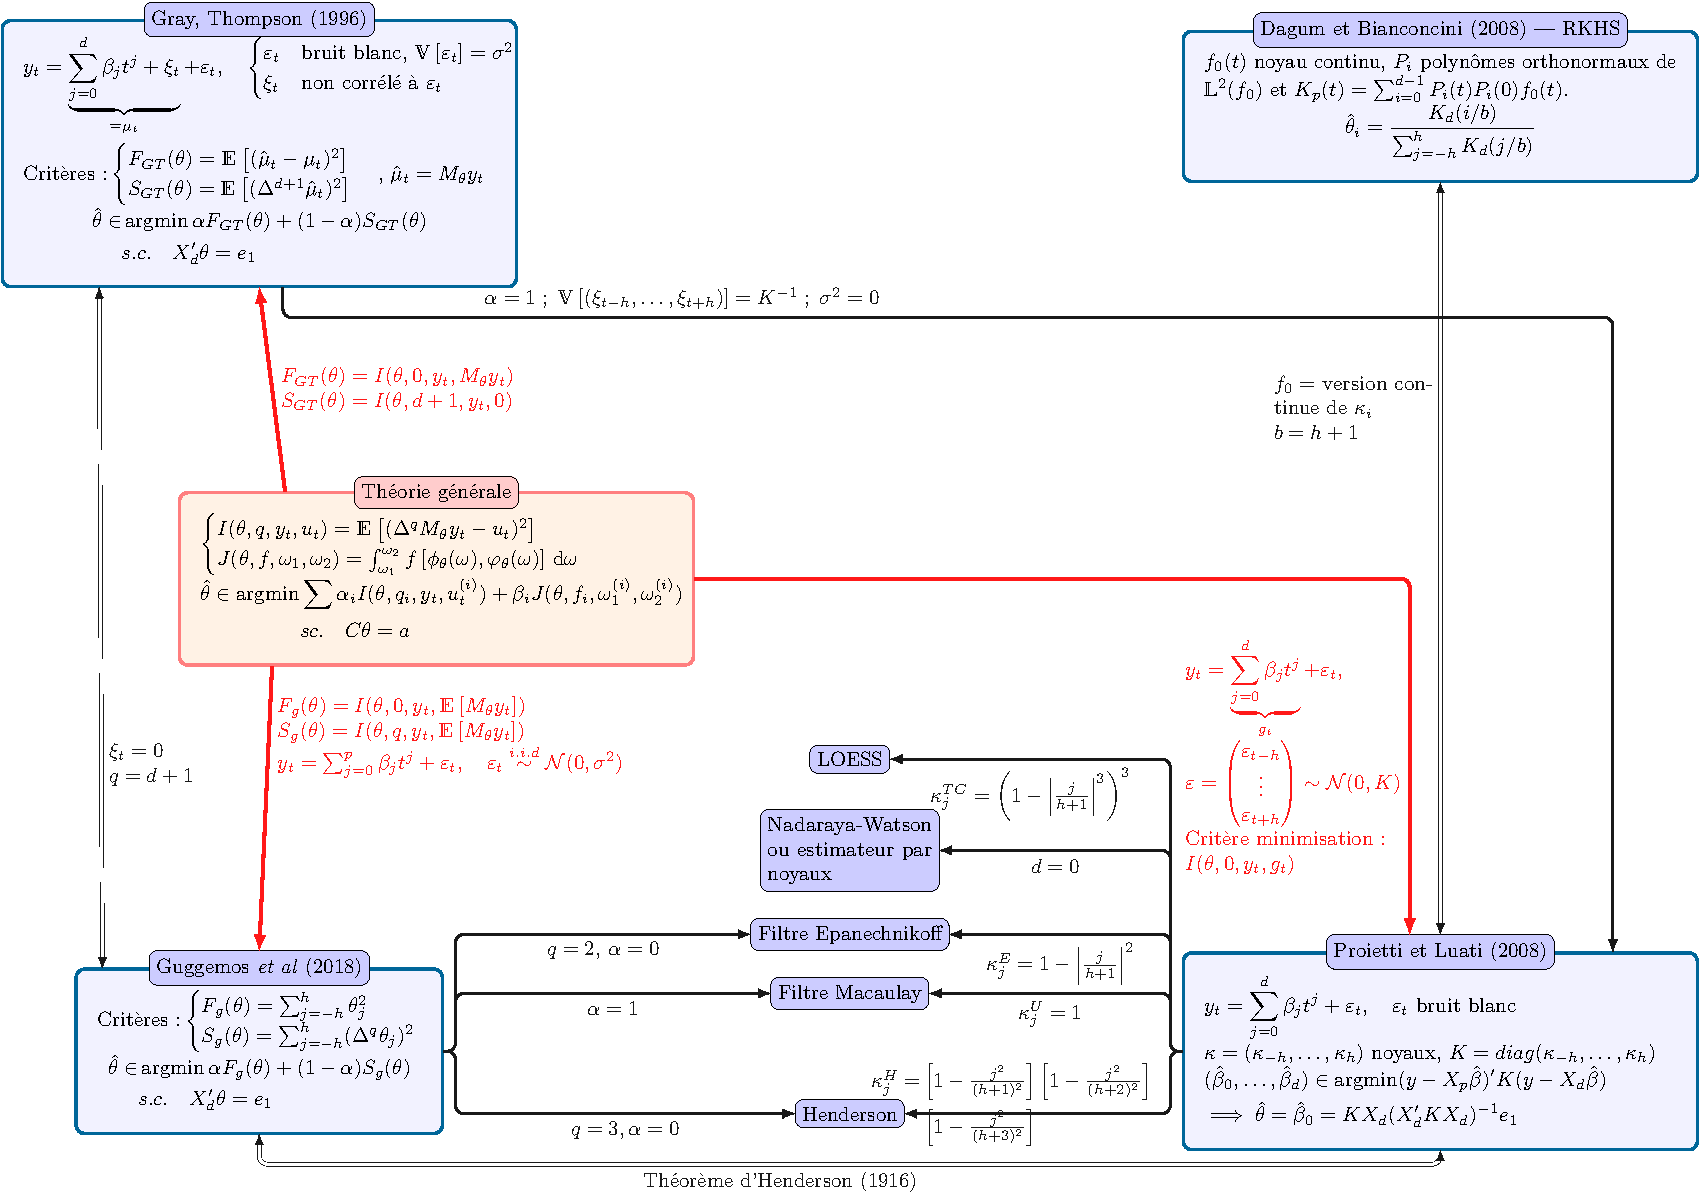
\includegraphics[width=0.9\textheight,angle=90]{img/bookdown/pdf/diag-gen-sym-1} 

}

\caption[Synthèse des méthodes de construction de moyennes mobiles symétriques \(\theta=(\theta_{-h},\dots,\theta_{h})\) de \(2h+1\) termes]{Synthèse des méthodes de construction de moyennes mobiles symétriques \(\theta=(\theta_{-h},\dots,\theta_{h})\) de \(2h+1\) termes.}\label{fig:diag-gen-sym}

\footnotesize


\emph{Note de lecture} : \emph{\(X = X_d = \begin{pmatrix} x_0 \quad\cdots \quad x_d \end{pmatrix}\) avec \(x_i'=\begin{pmatrix} (-h)^i \quad \cdots \quad (h)^i\end{pmatrix}\).}
\normalsize\end{figure}

\begin{figure}

{\centering 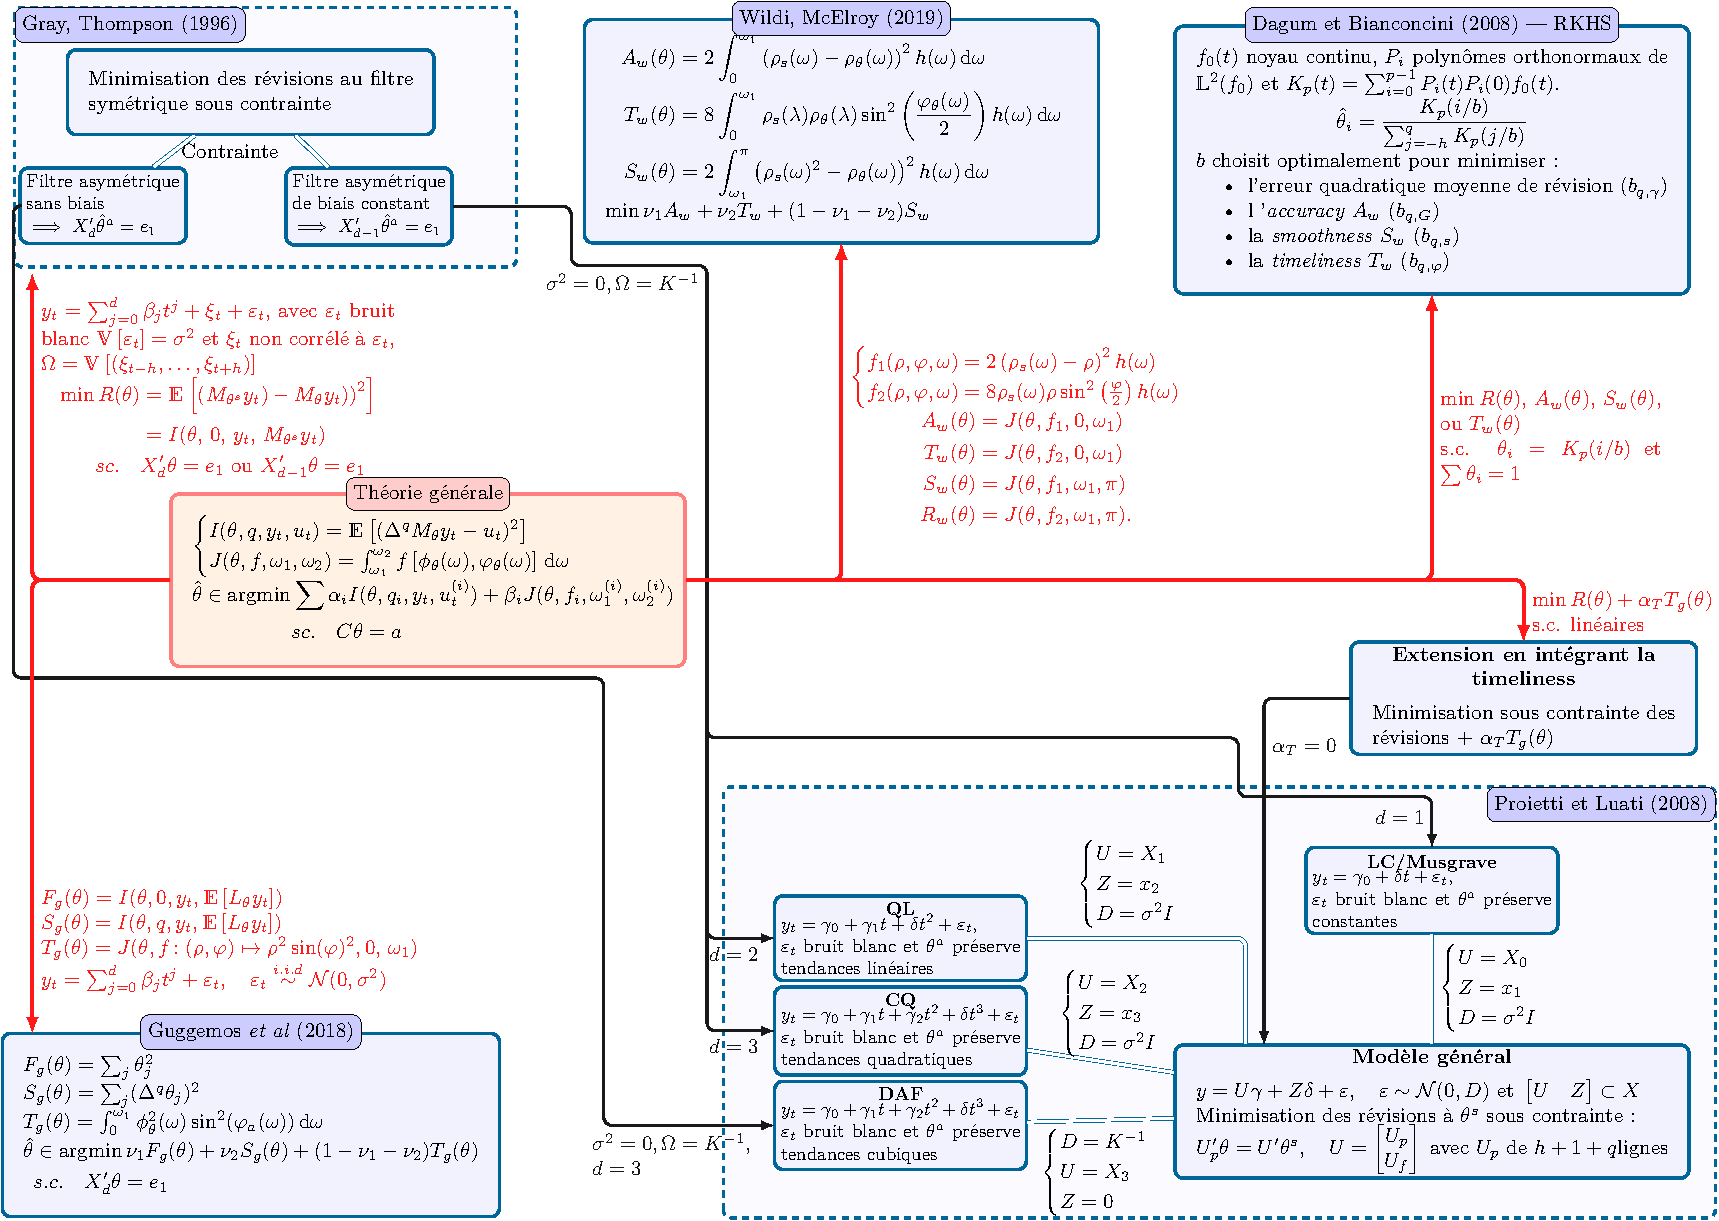
\includegraphics[width=0.9\textheight,angle=90]{img/bookdown/pdf/diag-gen-asym-1} 

}

\caption[Synthèse des méthodes de construction de moyennes mobiles asymétriques \(\theta=(\theta_{-h},\dots,\theta_{q})\), \(0\leq q< h\) avec \(\theta^s\) le filtre symétrique de référence de \(2h+1\) termes]{Synthèse des méthodes de construction de moyennes mobiles asymétriques \(\theta=(\theta_{-h},\dots,\theta_{q})\), \(0\leq q< h\) avec \(\theta^s\) le filtre symétrique de référence de \(2h+1\) termes.}\label{fig:diag-gen-asym}

\footnotesize


\emph{Note de lecture} : \emph{\(X_d = \begin{pmatrix} x_0 \quad\cdots \quad x_d \end{pmatrix}\) avec \(x_i'=\begin{pmatrix} (-h)^i \quad \cdots \quad (q)^i\end{pmatrix}\) et \(X=X_d\) avec \(q=h\).}
\normalsize\end{figure}

\newpage

\hypertarget{an-graphs}{%
\section{Coefficients, fonctions de gain et de déphasage}\label{an-graphs}}

\begin{figure}[H]

{\centering 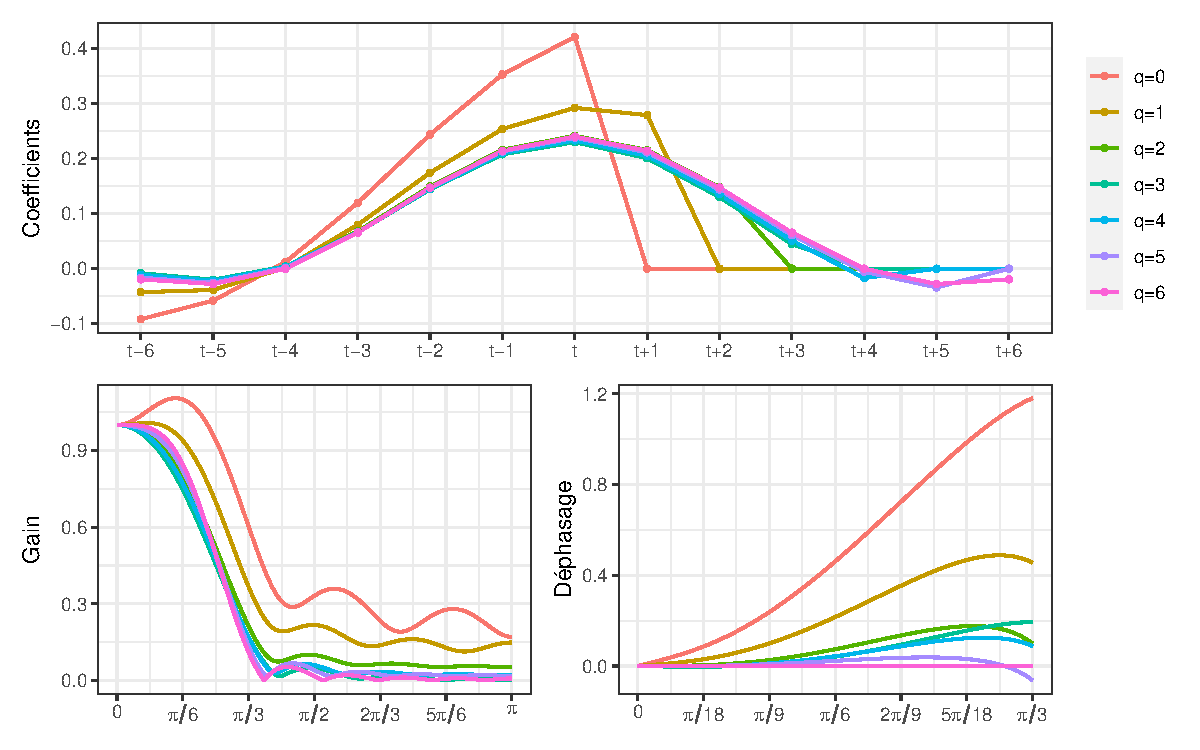
\includegraphics[width=1\linewidth]{img/filters_used/lc} 

}

\caption[Coefficients, fonctions de gain et de déphasage pour le filtre \emph{Linear-Constant} (LC) avec \(I/C=3,5\)]{Coefficients, fonctions de gain et de déphasage pour le filtre \emph{Linear-Constant} (LC) avec \(I/C=3,5\).}\label{fig:graphslc}

\footnotesize
\normalsize\end{figure}

\begin{figure}[H]

{\centering 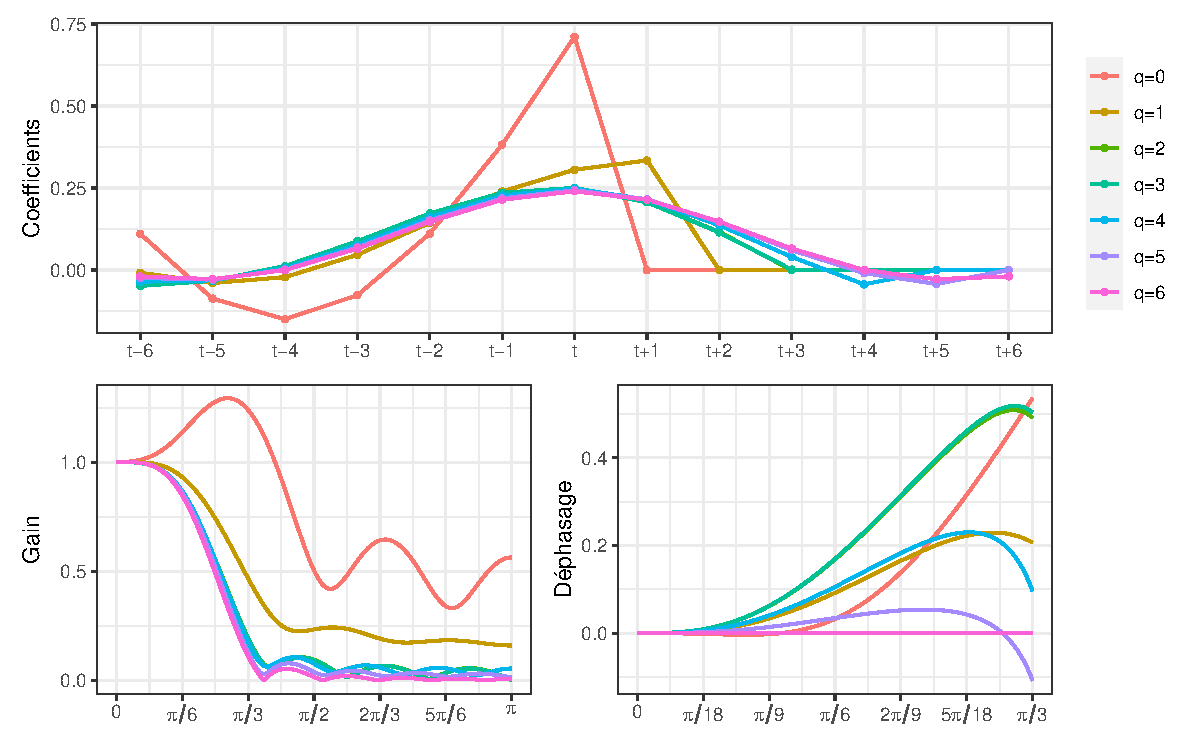
\includegraphics[width=1\linewidth]{img/filters_used/ql} 

}

\caption[Coefficients, fonctions de gain et de déphasage pour le filtre \emph{Quadratic-Linear} (QL) avec \(I/C=3,5\)]{Coefficients, fonctions de gain et de déphasage pour le filtre \emph{Quadratic-Linear} (QL) avec \(I/C=3,5\).}\label{fig:graphsql}

\footnotesize
\normalsize\end{figure}

\begin{figure}[H]

{\centering 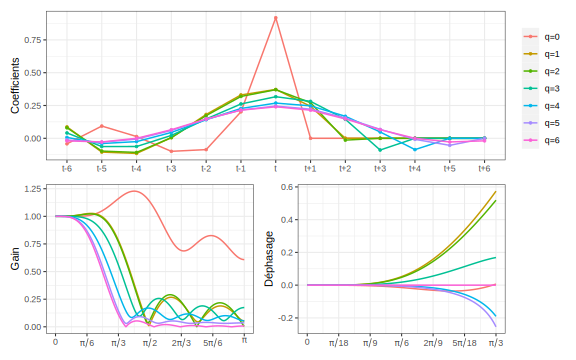
\includegraphics[width=1\linewidth]{img/filters_used/cq} 

}

\caption[Coefficients, fonctions de gain et de déphasage pour le filtre \emph{Cubic-Quadratic} (QL) avec \(I/C=3,5\)]{Coefficients, fonctions de gain et de déphasage pour le filtre \emph{Cubic-Quadratic} (QL) avec \(I/C=3,5\).}\label{fig:graphscq}

\footnotesize
\normalsize\end{figure}

\begin{figure}[H]

{\centering 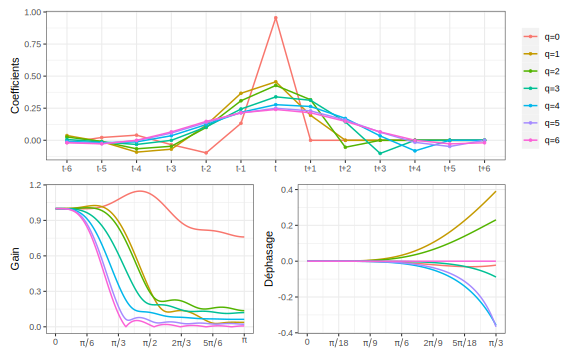
\includegraphics[width=1\linewidth]{img/filters_used/daf} 

}

\caption[Coefficients, fonctions de gain et de déphasage pour le filtre asymétrique direct (DAF) avec \(I/C=3,5\)]{Coefficients, fonctions de gain et de déphasage pour le filtre asymétrique direct (DAF) avec \(I/C=3,5\).}\label{fig:graphsdaf}

\footnotesize
\normalsize\end{figure}

\begin{figure}[H]

{\centering 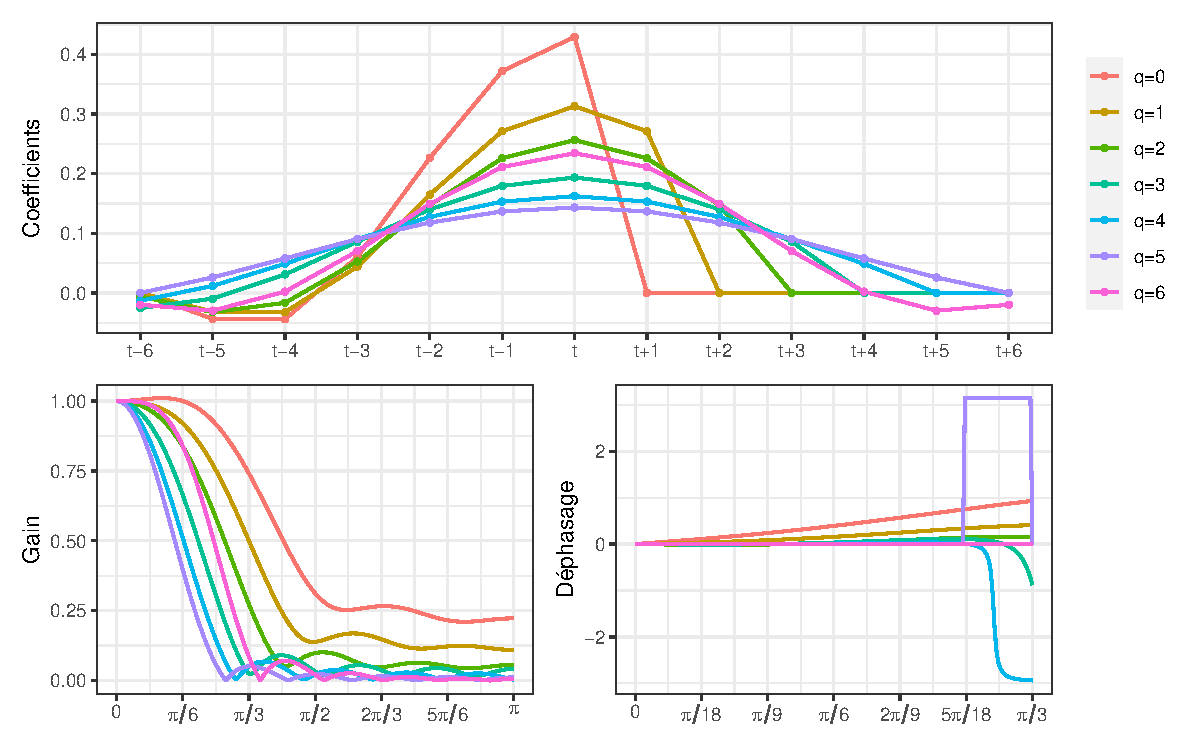
\includegraphics[width=1\linewidth]{img/filters_used/rkhs_timeliness} 

}

\caption[Coefficients, fonctions de gain et de déphasage pour le filtre RKHS \(b_{q,\varphi}\)]{Coefficients, fonctions de gain et de déphasage pour le filtre RKHS \(b_{q,\varphi}\).}\label{fig:graphsrkhs}

\footnotesize
\normalsize\end{figure}

\begin{figure}[H]

{\centering 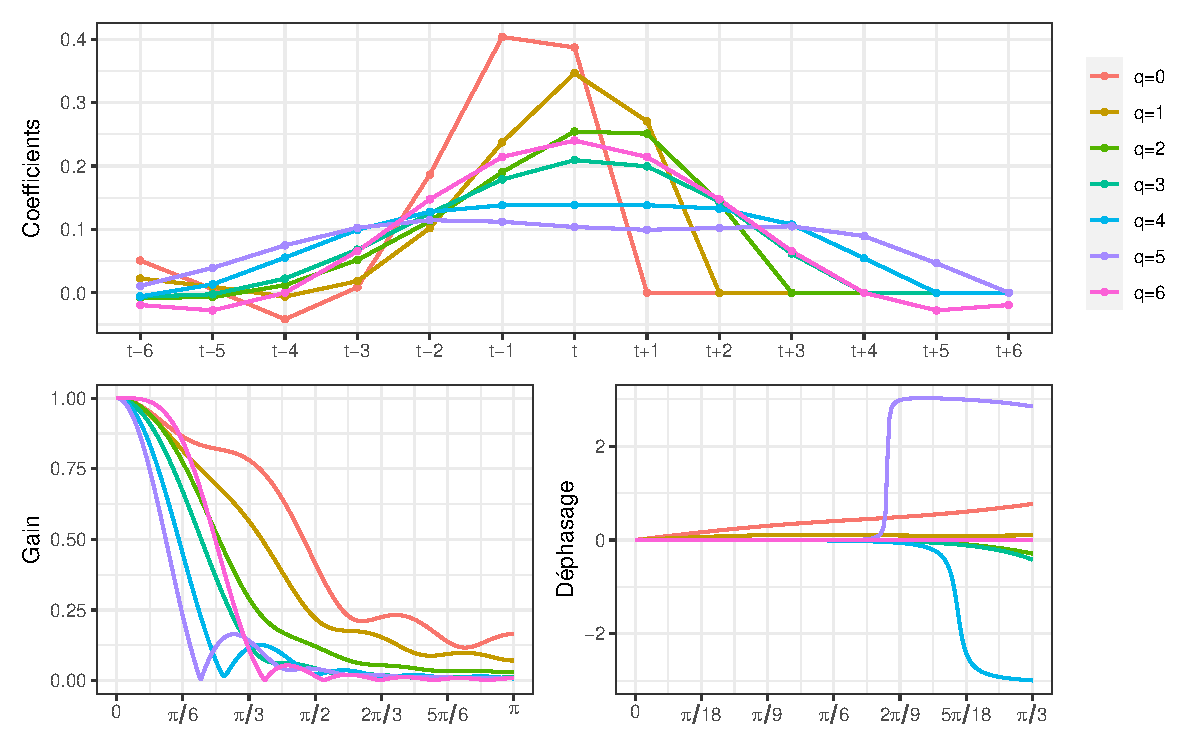
\includegraphics[width=1\linewidth]{img/filters_used/fst_lc} 

}

\caption[Coefficients, fonctions de gain et de déphasage pour le filtre FST optimal par rapport au filtre LC et minimisant la \emph{timeliness}]{Coefficients, fonctions de gain et de déphasage pour le filtre FST optimal par rapport au filtre LC et minimisant la \emph{timeliness}.}\label{fig:graphsfstlcmax}

\footnotesize
\normalsize\end{figure}

\begin{figure}[H]

{\centering 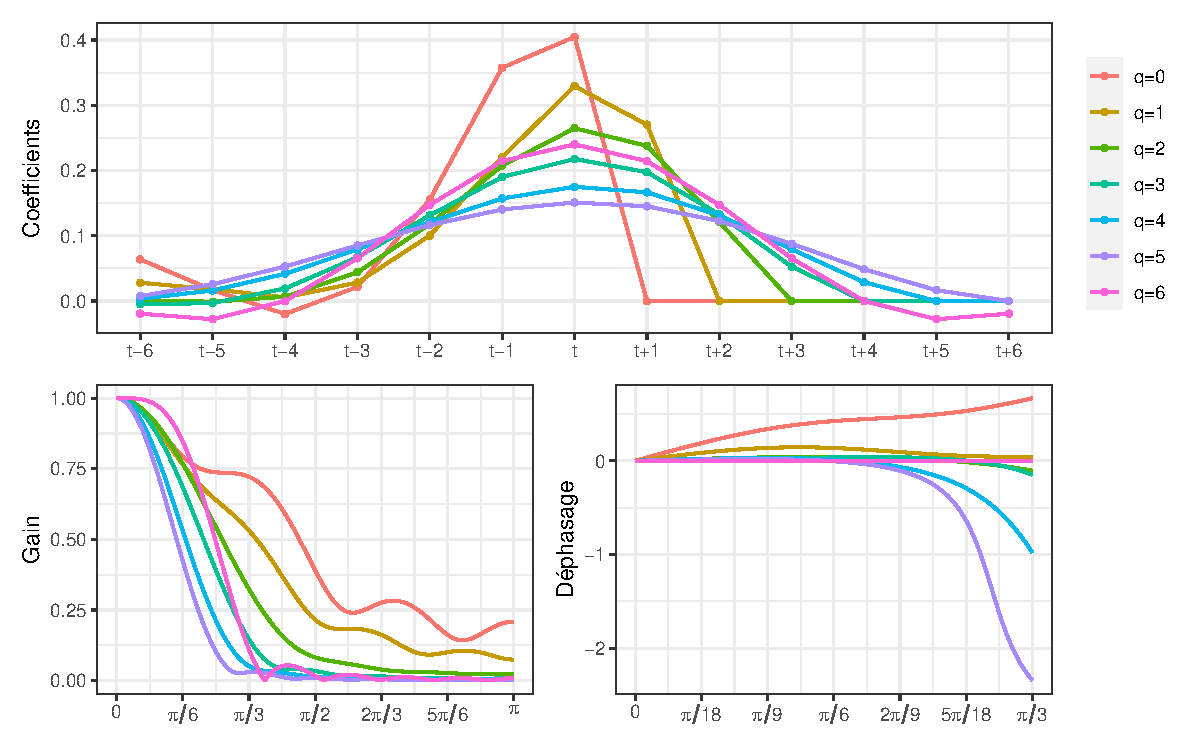
\includegraphics[width=1\linewidth]{img/filters_used/fst_lc_min} 

}

\caption[Coefficients, fonctions de gain et de déphasage pour le filtre FST optimal par rapport au filtre LC et ayant la \emph{timeliness} la plus élevée]{Coefficients, fonctions de gain et de déphasage pour le filtre FST optimal par rapport au filtre LC et ayant la \emph{timeliness} la plus élevée.}\label{fig:graphsfstlcmin}

\footnotesize
\normalsize\end{figure}

\begin{figure}[H]

{\centering 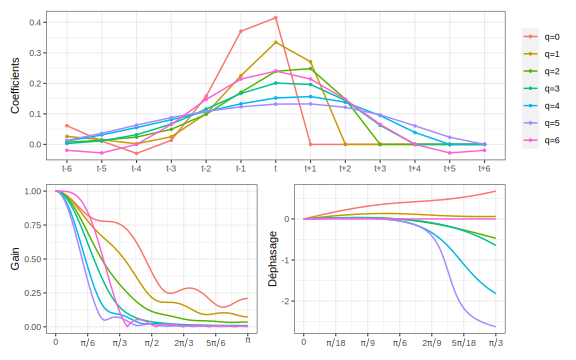
\includegraphics[width=1\linewidth]{img/filters_used/fst_lc_med} 

}

\caption[Coefficients, fonctions de gain et de déphasage pour le filtre FST optimal par rapport au filtre LC et ayant une \emph{timeliness} médiane]{Coefficients, fonctions de gain et de déphasage pour le filtre FST optimal par rapport au filtre LC et ayant une \emph{timeliness} médiane.}\label{fig:graphsfstlcmed}

\footnotesize
\normalsize\end{figure}

\begin{figure}[H]

{\centering 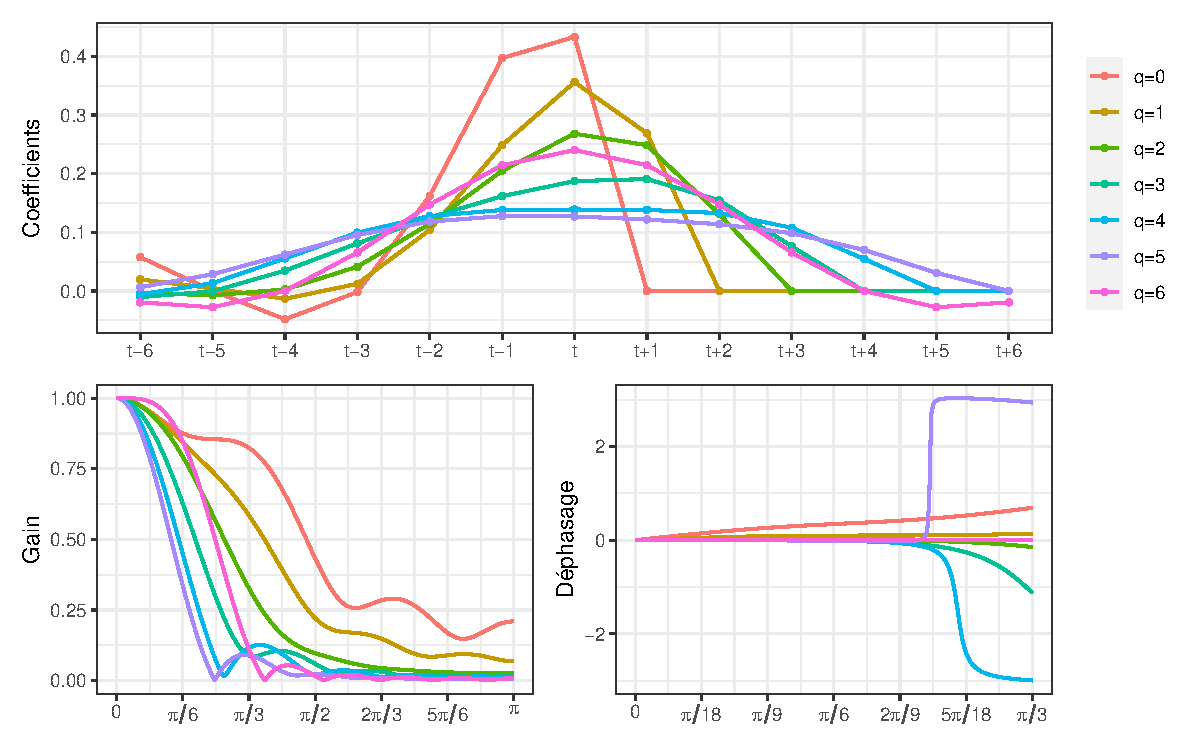
\includegraphics[width=1\linewidth]{img/filters_used/fst_rkhs_timeliness} 

}

\caption[Coefficients, fonctions de gain et de déphasage pour le filtre FST optimal par rapport au filtre RKHS \(b_{q,\varphi}\) et minimisant la \emph{timeliness}]{Coefficients, fonctions de gain et de déphasage pour le filtre FST optimal par rapport au filtre RKHS \(b_{q,\varphi}\) et minimisant la \emph{timeliness}.}\label{fig:graphsfstrkhs}

\footnotesize
\normalsize\end{figure}

\newpage

\hypertarget{an-equivfstlp}{%
\section{Équivalence entre l'approche FST et les filtres polynomiaux locaux}\label{an-equivfstlp}}

Dans cette annexe sont tracés les rares poids pour lesquels l'approche FST \textbf{n'est pas} équivalente à l'approche polynomiale locale, pour \(h=6\) (filtre symétrique de 13 termes) et \(h=11\) (filtre symétrique de 23 termes).
Lorsqu'un graphique n'est pas affiché c'est que tous les filtres FST sont équivalents une approche polynomiale locale par moindre carrés pondérés.
Par exemple pour les filtres associés au filtre symétrique de 13 termes (\(h=6\), figure \ref{fig:thhendersonh6}) il n'y a des graphiques que pour les filtres utilisés en temps réel (\(q=0\)) et lorsque ce filtre conserve les constantes (\(d=0\)), les droites (\(d=1\)) et les polynômes de degré 2 (\(d=2\)).
Dans tous les autres cas (i.e.; dès que l'on connait au moins un point dans le futur, \(q\geq 1\)), il y a équivalence pour tous les poids testés\footnote{
  Un quadrillage de 200 points de l'intervalle \([0,1]\) a été effectuée et on ne garde que l'ensemble des poids tels que leur somme fasse 1.}.

La \emph{smoothness} est calculée avec le paramètre \(q=3\) (\(S_g(\theta) = \sum_{j}(\nabla^{3}\theta_{j})^{2}\)), comme pour le filtre symétrique d'Henderson.

\begin{figure}[H]

{\centering 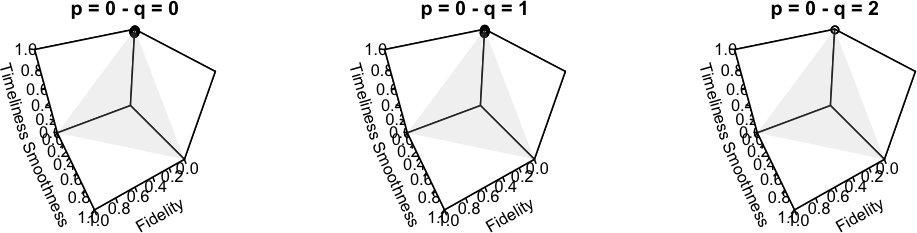
\includegraphics{img/bookdown/pdf/thhendersonh6-1} 

}

\caption[Ensemble des poids pour lesquels la méthode FST n'est pas équivalente aux moindres carrés pondérés pour \(h=6\) (filtre symétrique de 13 termes), sous contrainte de préservation des polynômes de degré au plus 2 (\(d=0,1,2\))]{Ensemble des poids pour lesquels la méthode FST n'est pas équivalente aux moindres carrés pondérés pour \(h=6\) (filtre symétrique de 13 termes), sous contrainte de préservation des polynômes de degré au plus 2 (\(d=0,1,2\)).}\label{fig:thhendersonh6}

\footnotesize
\normalsize\end{figure}

\begin{figure}[H]

{\centering 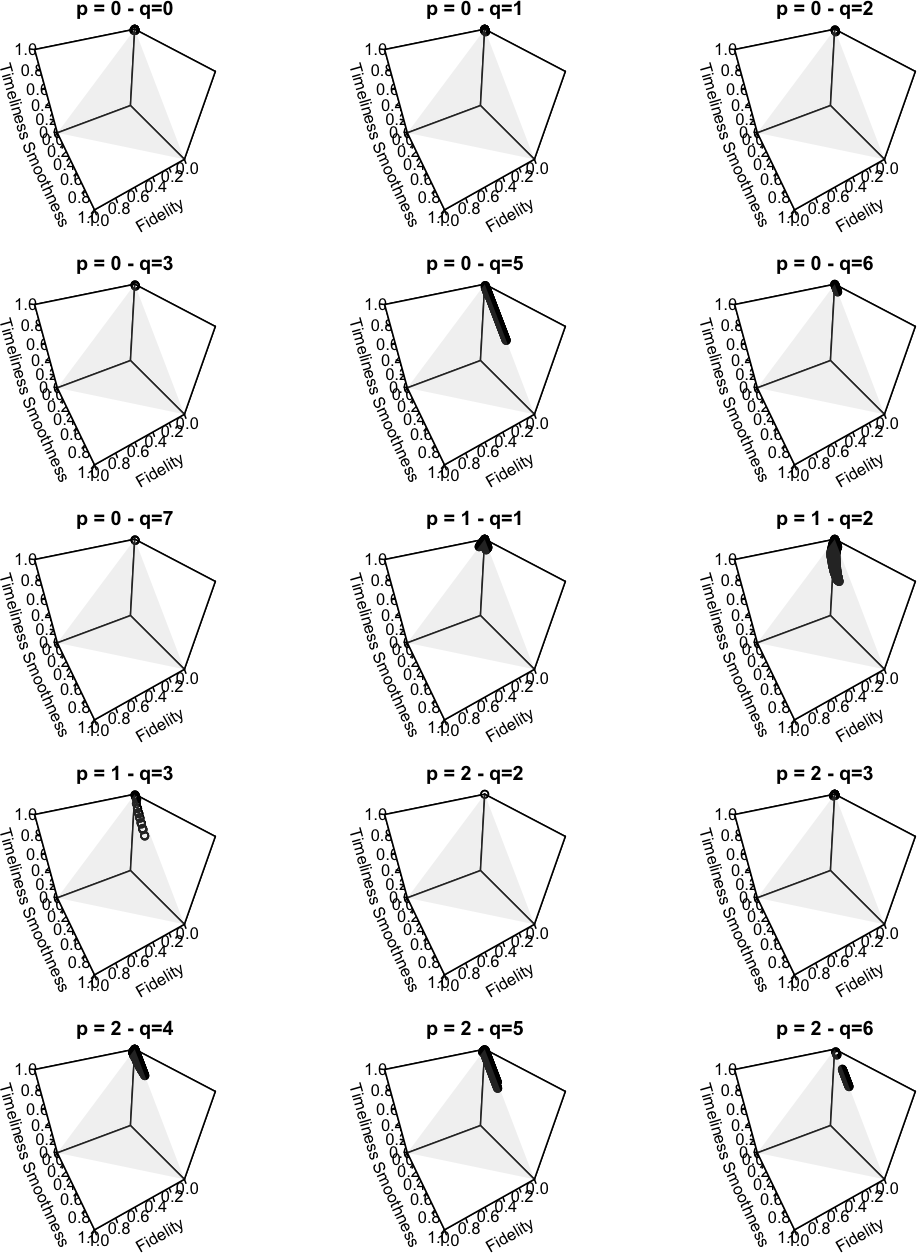
\includegraphics{img/bookdown/pdf/thhendersonh11d01-1} 

}

\caption[Ensemble des poids pour lesquels la méthode FST n'est pas équivalente aux moindres carrés pondérés pour \(h=11\) (filtre symétrique de 23 termes), sous contrainte de préservation des polynômes de degré au plus 2 (\(d=0,1,2\))]{Ensemble des poids pour lesquels la méthode FST n'est pas équivalente aux moindres carrés pondérés pour \(h=11\) (filtre symétrique de 23 termes), sous contrainte de préservation des polynômes de degré au plus 2 (\(d=0,1,2\)).}\label{fig:thhendersonh11d01}

\footnotesize
\normalsize\end{figure}

\newpage

\hypertarget{an-minrkhs}{%
\section{Critères de minimisation dans les filtres RKHS}\label{an-minrkhs}}

Cette annexe montre la fonction objectif que l'on cherche à minimiser dans la construction des filtres asymétriques par la méthode des RKHS.
Utiliser, dans le calcul des critères, la densité spectrale d'une marche aléatoire a peu d'influence sur la valeur des critères.

\hypertarget{filtre-symuxe9trique-de-9-termes-h4}{%
\subsection{\texorpdfstring{Filtre symétrique de 9 termes (\(h=4\))}{Filtre symétrique de 9 termes (h=4)}}\label{filtre-symuxe9trique-de-9-termes-h4}}

\begin{figure}[H]

{\centering 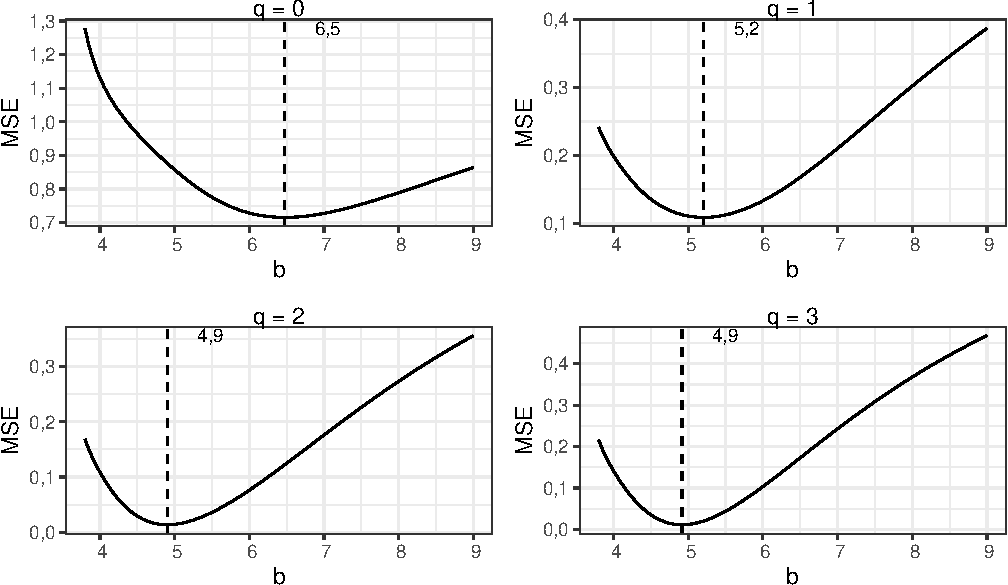
\includegraphics{img/bookdown/pdf/rkhsoptimse4wn-1} 

}

\caption[Erreur quadratique moyenne pour les filtres RKHS avec \(h_{WN}(x)=1\) (série initiale est un bruit blanc) en fonction du paramètre \(b\) pour un filtre symétrique de 9 termes]{Erreur quadratique moyenne pour les filtres RKHS avec \(h_{WN}(x)=1\) (série initiale est un bruit blanc) en fonction du paramètre \(b\) pour un filtre symétrique de 9 termes.}\label{fig:rkhsoptimse4wn}

\footnotesize


\emph{Notes} : \emph{Le trait horizontal correspond à la valeur obtenue par défaut dans rjdfilters.}

\emph{Dans la définition des indicateurs \(\omega_1=2\pi/12\).}
\normalsize\end{figure}

\begin{figure}[H]

{\centering 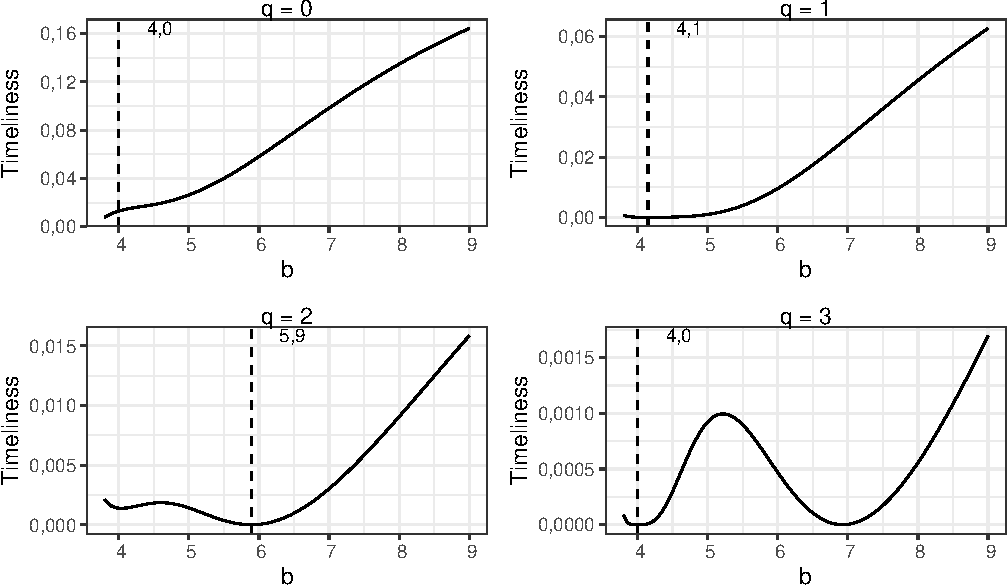
\includegraphics{img/bookdown/pdf/rkhstimeliness4wn-1} 

}

\caption[\emph{Timeliness} pour les filtres RKHS avec \(h_{WN}(x)=1\) (série initiale est un bruit blanc) en fonction du paramètre \(b\) pour un filtre symétrique de 9 termes]{\emph{Timeliness} pour les filtres RKHS avec \(h_{WN}(x)=1\) (série initiale est un bruit blanc) en fonction du paramètre \(b\) pour un filtre symétrique de 9 termes.}\label{fig:rkhstimeliness4wn}

\footnotesize


\emph{Notes} : \emph{Le trait horizontal correspond à la valeur obtenue par défaut dans rjdfilters.}

\emph{Dans la définition des indicateurs \(\omega_1=2\pi/12\).}
\normalsize\end{figure}

\begin{figure}[H]

{\centering 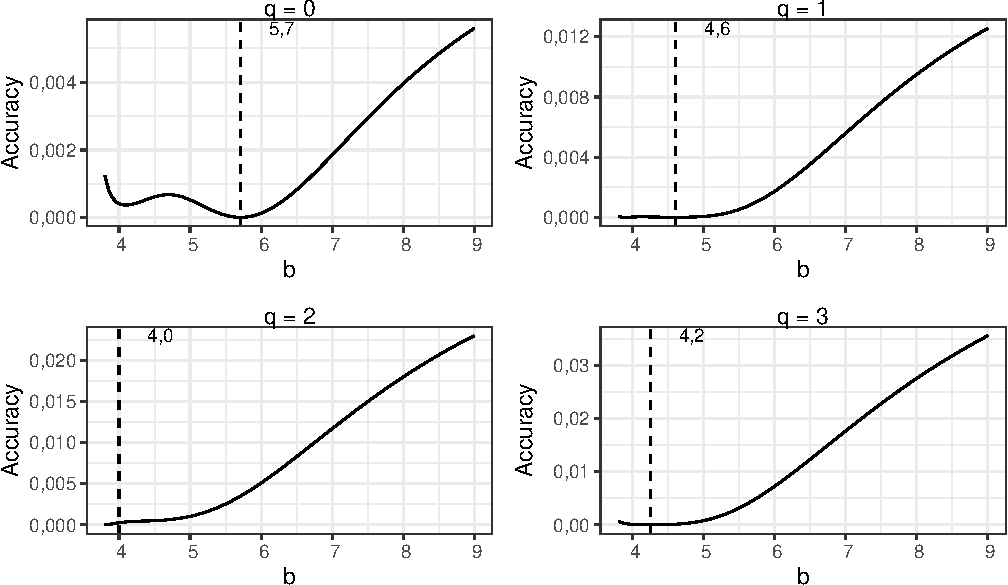
\includegraphics{img/bookdown/pdf/rkhsoptiaccuracy4wn-1} 

}

\caption[\emph{Accuracy} pour les filtres RKHS avec \(h_{WN}(x)=1\) (série initiale est un bruit blanc) en fonction du paramètre \(b\) pour un filtre symétrique de 9 termes]{\emph{Accuracy} pour les filtres RKHS avec \(h_{WN}(x)=1\) (série initiale est un bruit blanc) en fonction du paramètre \(b\) pour un filtre symétrique de 9 termes.}\label{fig:rkhsoptiaccuracy4wn}

\footnotesize


\emph{Notes} : \emph{Le trait horizontal correspond à la valeur obtenue par défaut dans rjdfilters.}

\emph{Dans la définition des indicateurs \(\omega_1=2\pi/12\).}
\normalsize\end{figure}

\begin{figure}[H]

{\centering 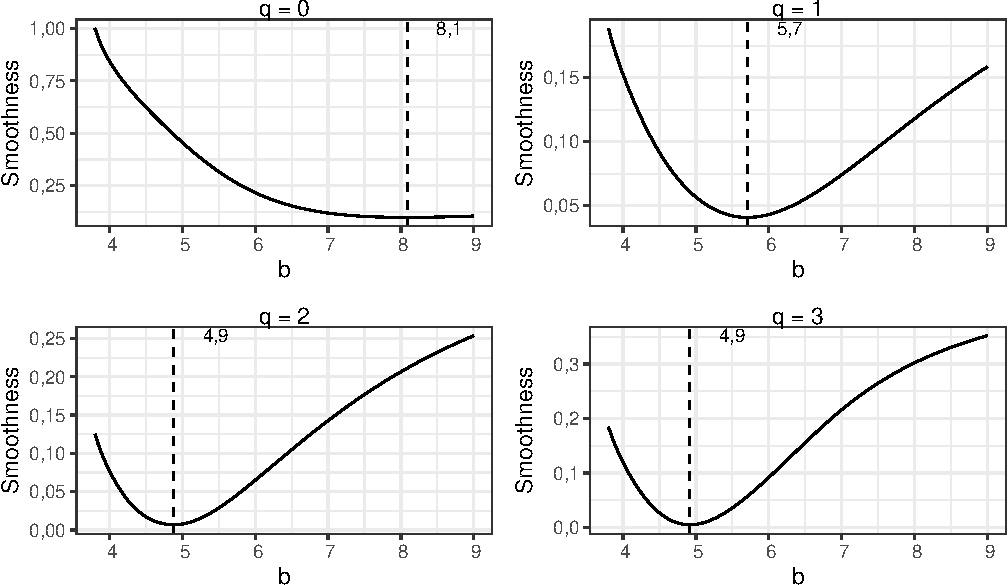
\includegraphics{img/bookdown/pdf/rkhsoptismoothness4wn-1} 

}

\caption[\emph{Smoothness} pour les filtres RKHS avec \(h_{WN}(x)=1\) (série initiale est un bruit blanc) en fonction du paramètre \(b\) pour un filtre symétrique de 9 termes]{\emph{Smoothness} pour les filtres RKHS avec \(h_{WN}(x)=1\) (série initiale est un bruit blanc) en fonction du paramètre \(b\) pour un filtre symétrique de 9 termes.}\label{fig:rkhsoptismoothness4wn}

\footnotesize


\emph{Notes} : \emph{Le trait horizontal correspond à la valeur obtenue par défaut dans rjdfilters.}

\emph{Dans la définition des indicateurs \(\omega_1=2\pi/12\).}
\normalsize\end{figure}

\newpage

\hypertarget{filtre-symuxe9trique-de-13-termes-h6}{%
\subsection{\texorpdfstring{Filtre symétrique de 13 termes (\(h=6\))}{Filtre symétrique de 13 termes (h=6)}}\label{filtre-symuxe9trique-de-13-termes-h6}}

\begin{figure}[H]

{\centering 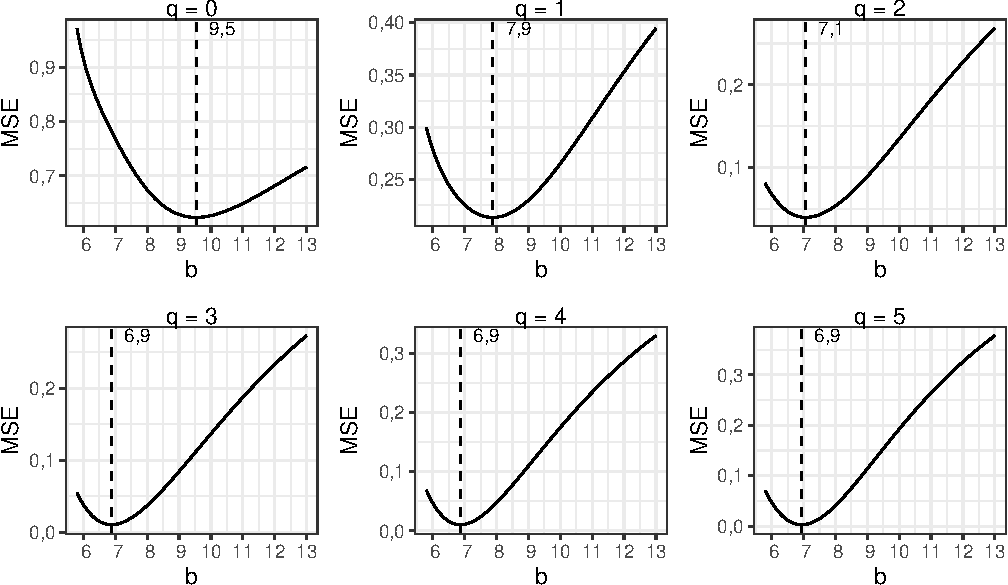
\includegraphics{img/bookdown/pdf/rkhsoptimse6wn-1} 

}

\caption[Erreur quadratique moyenne pour les filtres RKHS avec \(h_{WN}(x)=1\) (série initiale est un bruit blanc) en fonction du paramètre \(b\) pour un filtre symétrique de 13 termes]{Erreur quadratique moyenne pour les filtres RKHS avec \(h_{WN}(x)=1\) (série initiale est un bruit blanc) en fonction du paramètre \(b\) pour un filtre symétrique de 13 termes.}\label{fig:rkhsoptimse6wn}

\footnotesize


\emph{Notes} : \emph{Le trait horizontal correspond à la valeur obtenue par défaut dans rjdfilters.}

\emph{Dans la définition des indicateurs \(\omega_1=2\pi/12\).}
\normalsize\end{figure}

\begin{figure}[H]

{\centering 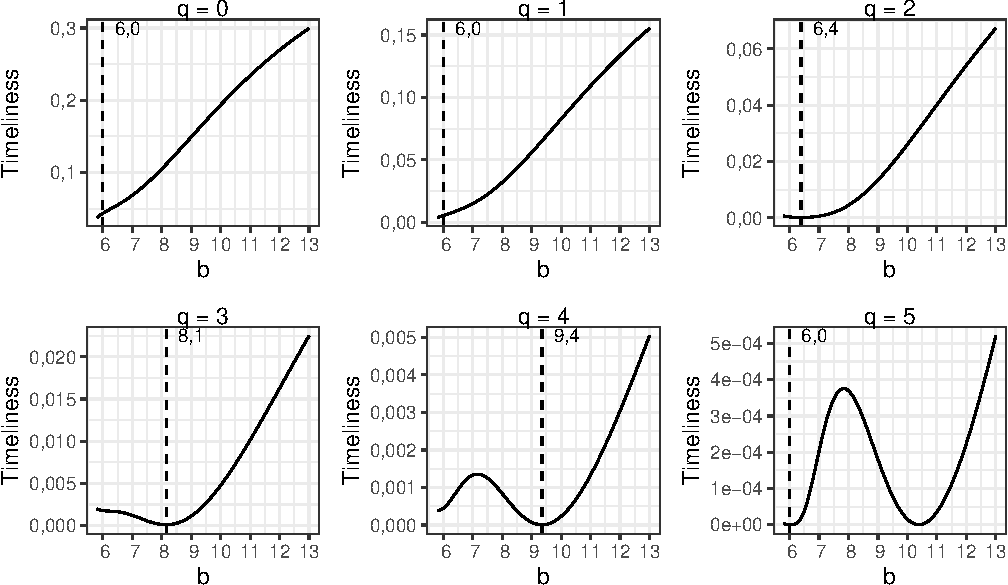
\includegraphics{img/bookdown/pdf/rkhstimeliness6wn-1} 

}

\caption[\emph{Timeliness} pour les filtres RKHS avec \(h_{WN}(x)=1\) (série initiale est un bruit blanc) en fonction du paramètre \(b\) pour un filtre symétrique de 13 termes]{\emph{Timeliness} pour les filtres RKHS avec \(h_{WN}(x)=1\) (série initiale est un bruit blanc) en fonction du paramètre \(b\) pour un filtre symétrique de 13 termes.}\label{fig:rkhstimeliness6wn}

\footnotesize


\emph{Notes} : \emph{Le trait horizontal correspond à la valeur obtenue par défaut dans rjdfilters.}

\emph{Dans la définition des indicateurs \(\omega_1=2\pi/12\).}
\normalsize\end{figure}

\begin{figure}[H]

{\centering 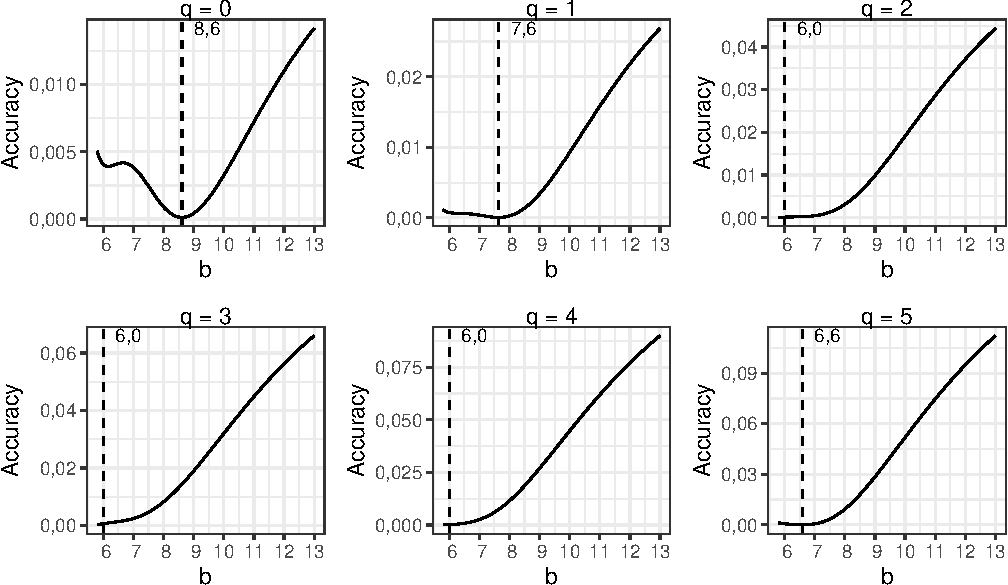
\includegraphics{img/bookdown/pdf/rkhsoptiaccuracy6wn-1} 

}

\caption[\emph{Accuracy} pour les filtres RKHS avec \(h_{WN}(x)=1\) (série initiale est un bruit blanc) en fonction du paramètre \(b\) pour un filtre symétrique de 13 termes]{\emph{Accuracy} pour les filtres RKHS avec \(h_{WN}(x)=1\) (série initiale est un bruit blanc) en fonction du paramètre \(b\) pour un filtre symétrique de 13 termes.}\label{fig:rkhsoptiaccuracy6wn}

\footnotesize


\emph{Notes} : \emph{Le trait horizontal correspond à la valeur obtenue par défaut dans rjdfilters.}

\emph{Dans la définition des indicateurs \(\omega_1=2\pi/12\).}
\normalsize\end{figure}

\begin{figure}[H]

{\centering 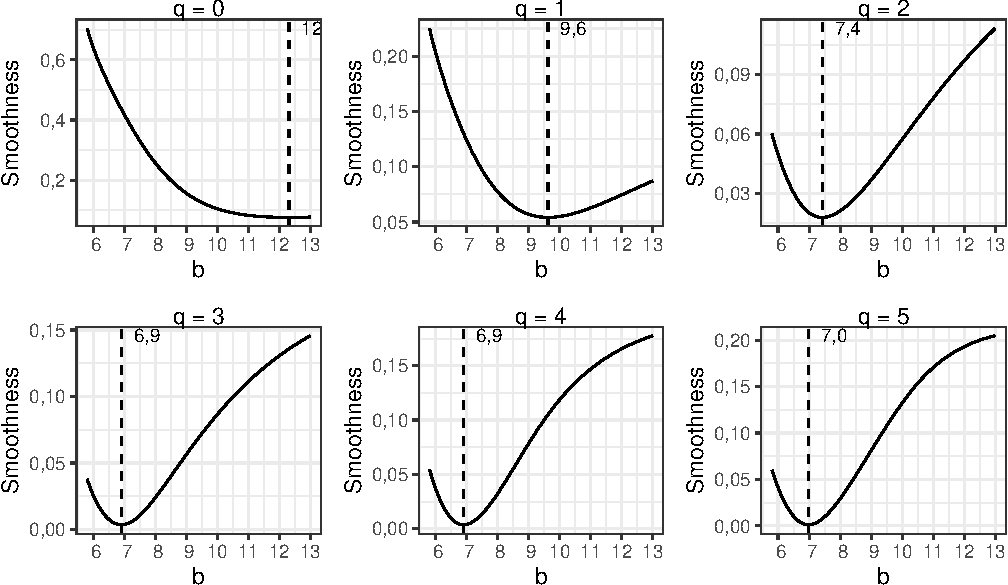
\includegraphics{img/bookdown/pdf/rkhsoptismoothness6wn-1} 

}

\caption[\emph{Smoothness} pour les filtres RKHS avec \(h_{WN}(x)=1\) (série initiale est un bruit blanc) en fonction du paramètre \(b\) pour un filtre symétrique de 13 termes]{\emph{Smoothness} pour les filtres RKHS avec \(h_{WN}(x)=1\) (série initiale est un bruit blanc) en fonction du paramètre \(b\) pour un filtre symétrique de 13 termes.}\label{fig:rkhsoptismoothness6wn}

\footnotesize


\emph{Notes} : \emph{Le trait horizontal correspond à la valeur obtenue par défaut dans rjdfilters.}

\emph{Dans la définition des indicateurs \(\omega_1=2\pi/12\).}
\normalsize\end{figure}

\newpage

\hypertarget{filtre-symuxe9trique-de-23-termes-h11}{%
\subsection{\texorpdfstring{Filtre symétrique de 23 termes (\(h=11\))}{Filtre symétrique de 23 termes (h=11)}}\label{filtre-symuxe9trique-de-23-termes-h11}}

\begin{figure}[H]

{\centering 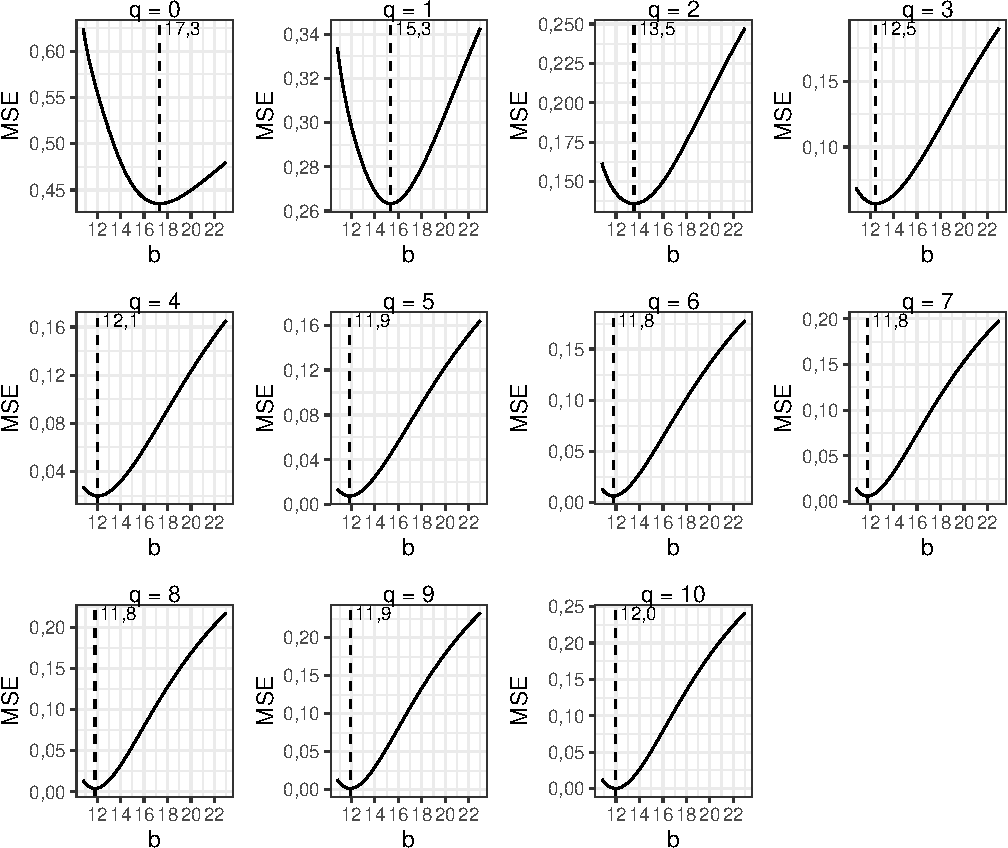
\includegraphics{img/bookdown/pdf/rkhsoptimse11wn-1} 

}

\caption[Erreur quadratique moyenne pour les filtres RKHS avec \(h_{WN}(x)=1\) (série initiale est un bruit blanc) en fonction du paramètre \(b\) pour un filtre symétrique de 23 termes]{Erreur quadratique moyenne pour les filtres RKHS avec \(h_{WN}(x)=1\) (série initiale est un bruit blanc) en fonction du paramètre \(b\) pour un filtre symétrique de 23 termes.}\label{fig:rkhsoptimse11wn}

\footnotesize


\emph{Notes} : \emph{Le trait horizontal correspond à la valeur obtenue par défaut dans rjdfilters.}

\emph{Dans la définition des indicateurs \(\omega_1=2\pi/12\).}
\normalsize\end{figure}

\begin{figure}[H]

{\centering 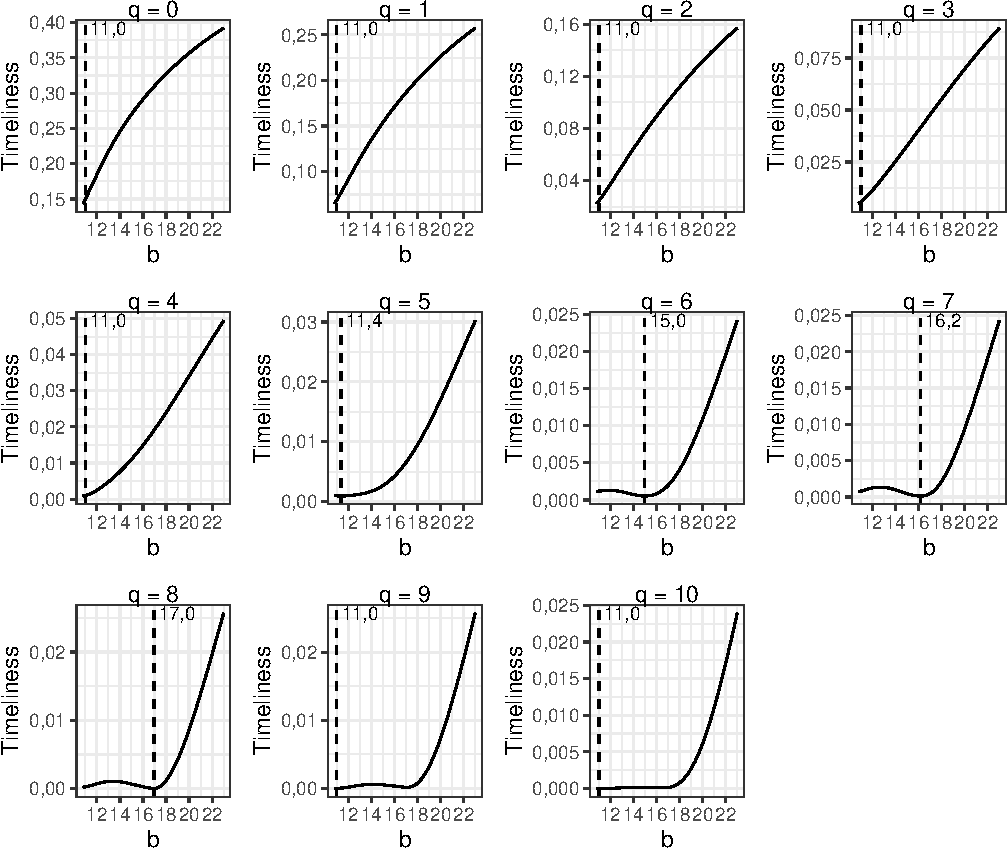
\includegraphics{img/bookdown/pdf/rkhstimeliness11wn-1} 

}

\caption[\emph{Timeliness} pour les filtres RKHS avec \(h_{WN}(x)=1\) (série initiale est un bruit blanc) en fonction du paramètre \(b\) pour un filtre symétrique de 23 termes]{\emph{Timeliness} pour les filtres RKHS avec \(h_{WN}(x)=1\) (série initiale est un bruit blanc) en fonction du paramètre \(b\) pour un filtre symétrique de 23 termes.}\label{fig:rkhstimeliness11wn}

\footnotesize


\emph{Notes} : \emph{Le trait horizontal correspond à la valeur obtenue par défaut dans rjdfilters.}

\emph{Dans la définition des indicateurs \(\omega_1=2\pi/12\).}
\normalsize\end{figure}

\begin{figure}[H]

{\centering 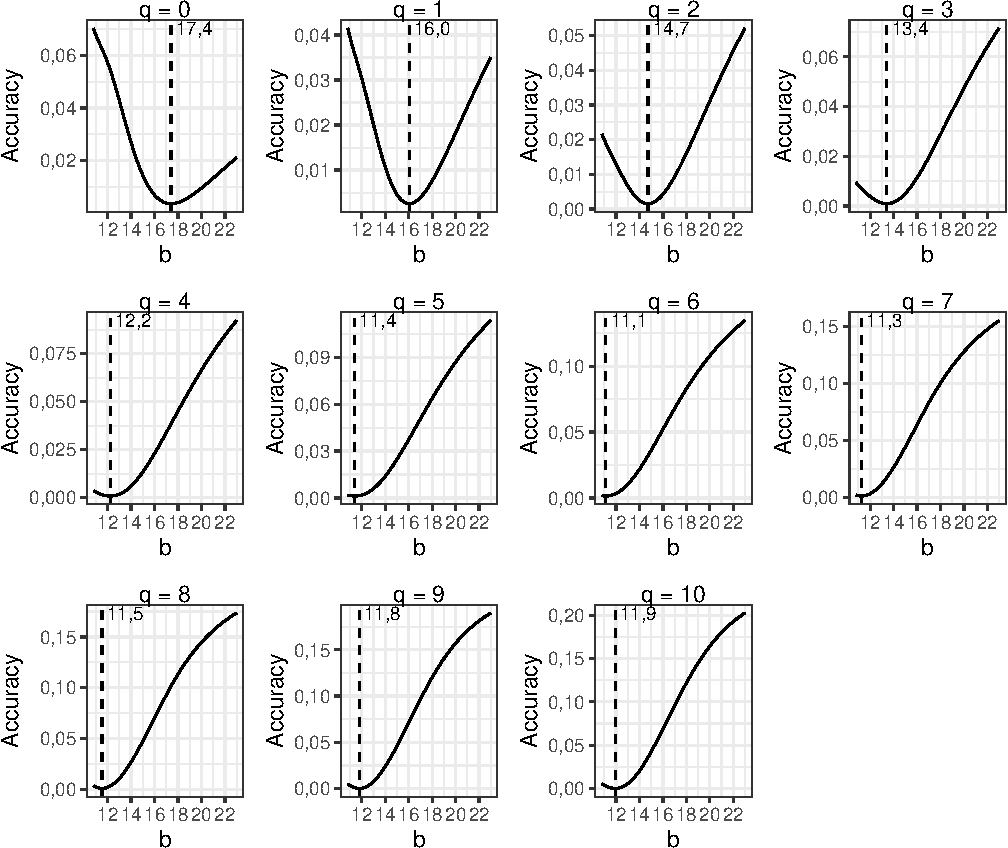
\includegraphics{img/bookdown/pdf/rkhsoptiaccuracy11wn-1} 

}

\caption[\emph{Accuracy} pour les filtres RKHS avec \(h_{WN}(x)=1\) (série initiale est un bruit blanc) en fonction du paramètre \(b\) pour un filtre symétrique de 23 termes]{\emph{Accuracy} pour les filtres RKHS avec \(h_{WN}(x)=1\) (série initiale est un bruit blanc) en fonction du paramètre \(b\) pour un filtre symétrique de 23 termes.}\label{fig:rkhsoptiaccuracy11wn}

\footnotesize


\emph{Notes} : \emph{Le trait horizontal correspond à la valeur obtenue par défaut dans rjdfilters.}

\emph{Dans la définition des indicateurs \(\omega_1=2\pi/12\).}
\normalsize\end{figure}

\begin{figure}[H]

{\centering 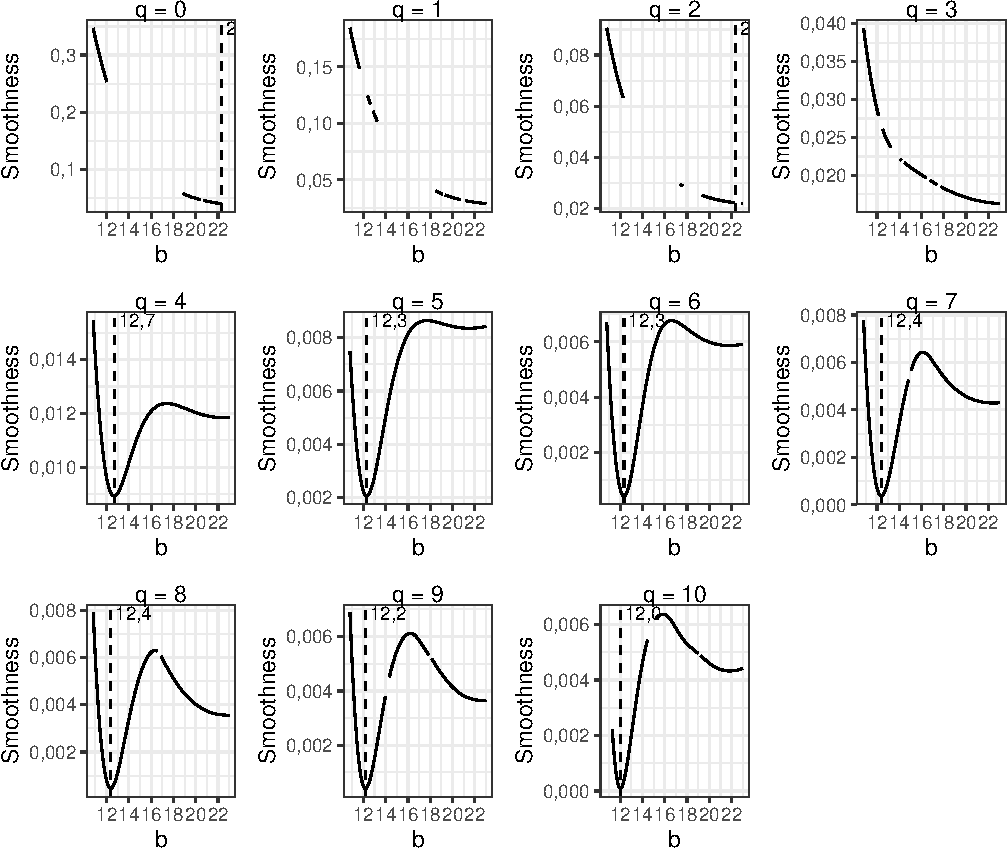
\includegraphics{img/bookdown/pdf/rkhsoptismoothness11wn-1} 

}

\caption[\emph{Smoothness} pour les filtres RKHS avec \(h_{WN}(x)=1\) (série initiale est un bruit blanc) en fonction du paramètre \(b\) pour un filtre symétrique de 23 termes]{\emph{Smoothness} pour les filtres RKHS avec \(h_{WN}(x)=1\) (série initiale est un bruit blanc) en fonction du paramètre \(b\) pour un filtre symétrique de 23 termes.}\label{fig:rkhsoptismoothness11wn}

\footnotesize


\emph{Notes} : \emph{Le trait horizontal correspond à la valeur obtenue par défaut dans rjdfilters.}

\emph{Dans la définition des indicateurs \(\omega_1=2\pi/12\).}
\normalsize\end{figure}

\newpage

\hypertarget{sec-annexeFST}{%
\section{Comparaison avec le filtre FST}\label{sec-annexeFST}}

Cette annexe synthétise les cas où il est possible de trouver un ensemble de poids tels que les filtres FST ont de meilleurs propriétés (en termes de \emph{fidelity}, \emph{smoothness} et \emph{timeliness}) que les filtres polynomiaux ou RKHS, avec les mêmes contraintes sur la préservation des polynômes (ou des contraintes supérieures).
Par simplicité, les graphiques ne sont tracés que pour les principales méthodes étudiées : le filtre \emph{Linear-Constant} (LC) et le filtre RKHS \(b_{q,\varphi}\) obtenu par minimisation de la \emph{timeliness}.
Pour les filtres LC, utiliser un I-C ratio à 3,5 ou 4,5 n'a quasiment aucun impact : pour synthétiser ces valeurs, ne sont tracés que les ensembles de poids qui donnent des filtres optimaux pour ces deux valeurs.

\hypertarget{filtres-polynomiaux-locaux}{%
\subsection{Filtres polynomiaux locaux}\label{filtres-polynomiaux-locaux}}

\begin{figure}[H]

{\centering 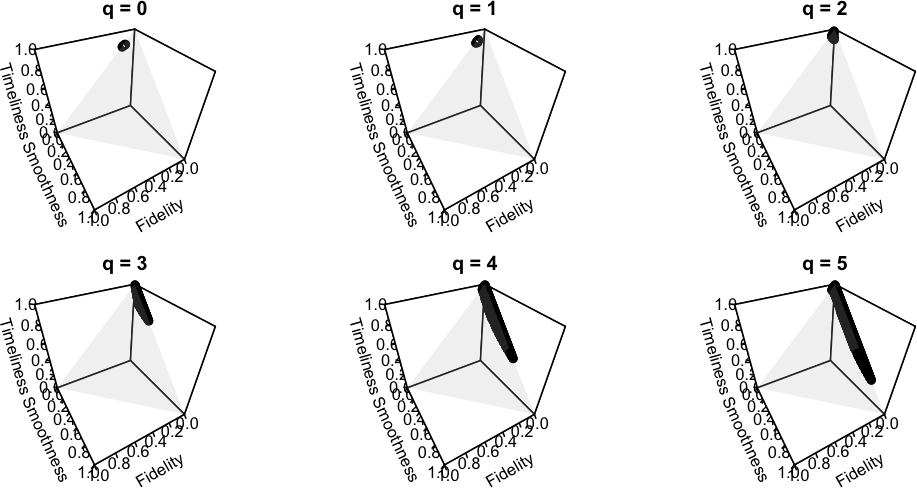
\includegraphics{img/bookdown/pdf/lc6d0-1} 

}

\caption[Ensemble des poids pour lesquels la méthode FST donne des filtres de meilleure qualité que le filtre \emph{Linear-Constant} (LC) sous contrainte de préservation des constantes (\(d=0\)) et pour \(h=6\)]{Ensemble des poids pour lesquels la méthode FST donne des filtres de meilleure qualité que le filtre \emph{Linear-Constant} (LC) sous contrainte de préservation des constantes (\(d=0\)) et pour \(h=6\).}\label{fig:lc6d0}

\footnotesize


\emph{Notes} : \emph{La zone grisée correspond à l'ensemble \(\left\{\begin{pmatrix}x \; y \; z \end{pmatrix}' : x+y+z=1\right\}\).}

\emph{Le graphique est vide lorsque aucun poids ne permet de trouver de filtre FST qui minimise la \emph{fidelity}, \emph{smoothness} et la \emph{timeliness} par rapport au filtre étudié.}
\normalsize\end{figure}

\begin{figure}[H]

{\centering 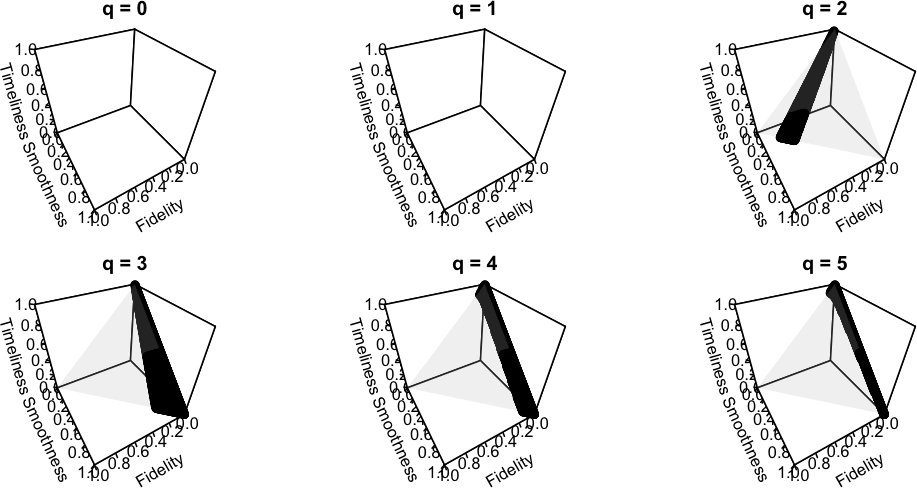
\includegraphics{img/bookdown/pdf/lc6d1-1} 

}

\caption[Ensemble des poids pour lesquels la méthode FST donne des filtres de meilleure qualité que le filtre \emph{Linear-Constant} (LC) sous contrainte de préservation des droites (\(d=1\)) et pour \(h=6\)]{Ensemble des poids pour lesquels la méthode FST donne des filtres de meilleure qualité que le filtre \emph{Linear-Constant} (LC) sous contrainte de préservation des droites (\(d=1\)) et pour \(h=6\).}\label{fig:lc6d1}

\footnotesize


\emph{Notes} : \emph{La zone grisée correspond à l'ensemble \(\left\{\begin{pmatrix}x \; y \; z \end{pmatrix}' : x+y+z=1\right\}\).}

\emph{Le graphique est vide lorsque aucun poids ne permet de trouver de filtre FST qui minimise la \emph{fidelity}, \emph{smoothness} et la \emph{timeliness} par rapport au filtre étudié.}
\normalsize\end{figure}

\begin{figure}[H]

{\centering 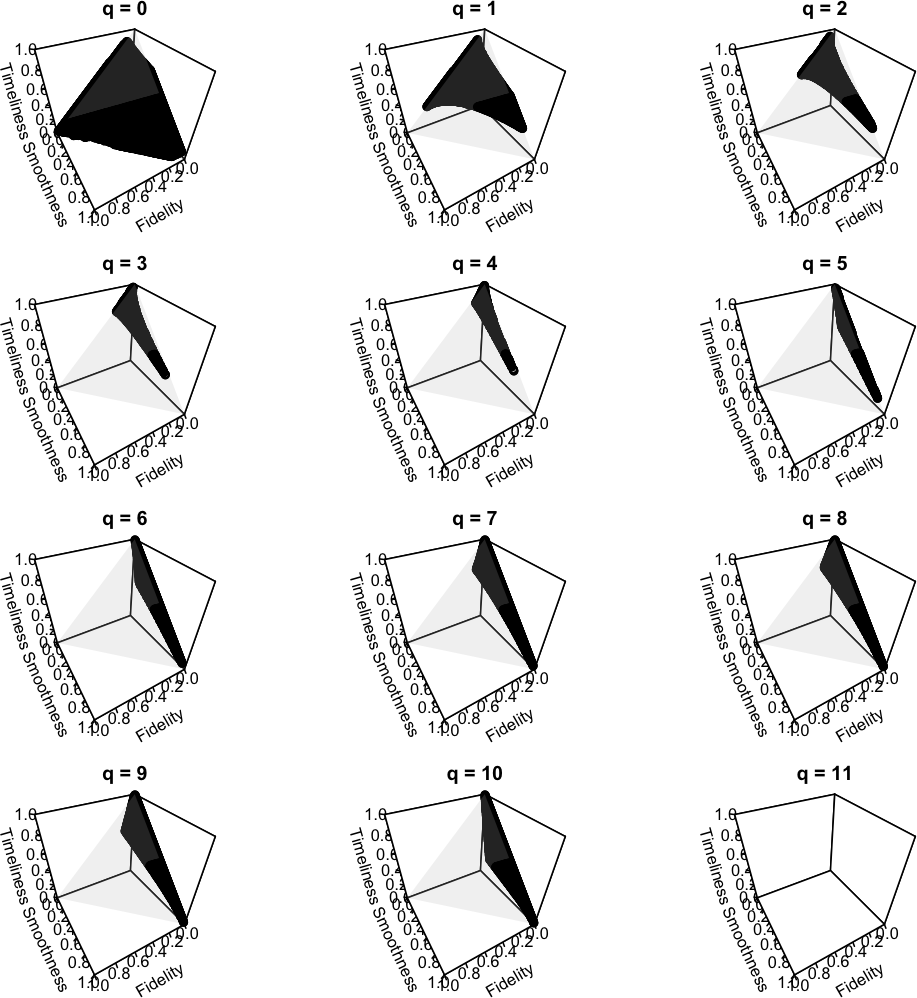
\includegraphics{img/bookdown/pdf/lc11d0-1} 

}

\caption[Ensemble des poids pour lesquels la méthode FST donne des filtres de meilleure qualité que le filtre \emph{Linear-Constant} (LC) sous contrainte de préservation des constantes (\(d=0\)) et pour \(h=11\)]{Ensemble des poids pour lesquels la méthode FST donne des filtres de meilleure qualité que le filtre \emph{Linear-Constant} (LC) sous contrainte de préservation des constantes (\(d=0\)) et pour \(h=11\).}\label{fig:lc11d0}

\footnotesize


\emph{Notes} : \emph{La zone grisée correspond à l'ensemble \(\left\{\begin{pmatrix}x \; y \; z \end{pmatrix}' : x+y+z=1\right\}\).}

\emph{Le graphique est vide lorsque aucun poids ne permet de trouver de filtre FST qui minimise la \emph{fidelity}, \emph{smoothness} et la \emph{timeliness} par rapport au filtre étudié.}
\normalsize\end{figure}

\begin{figure}[H]

{\centering 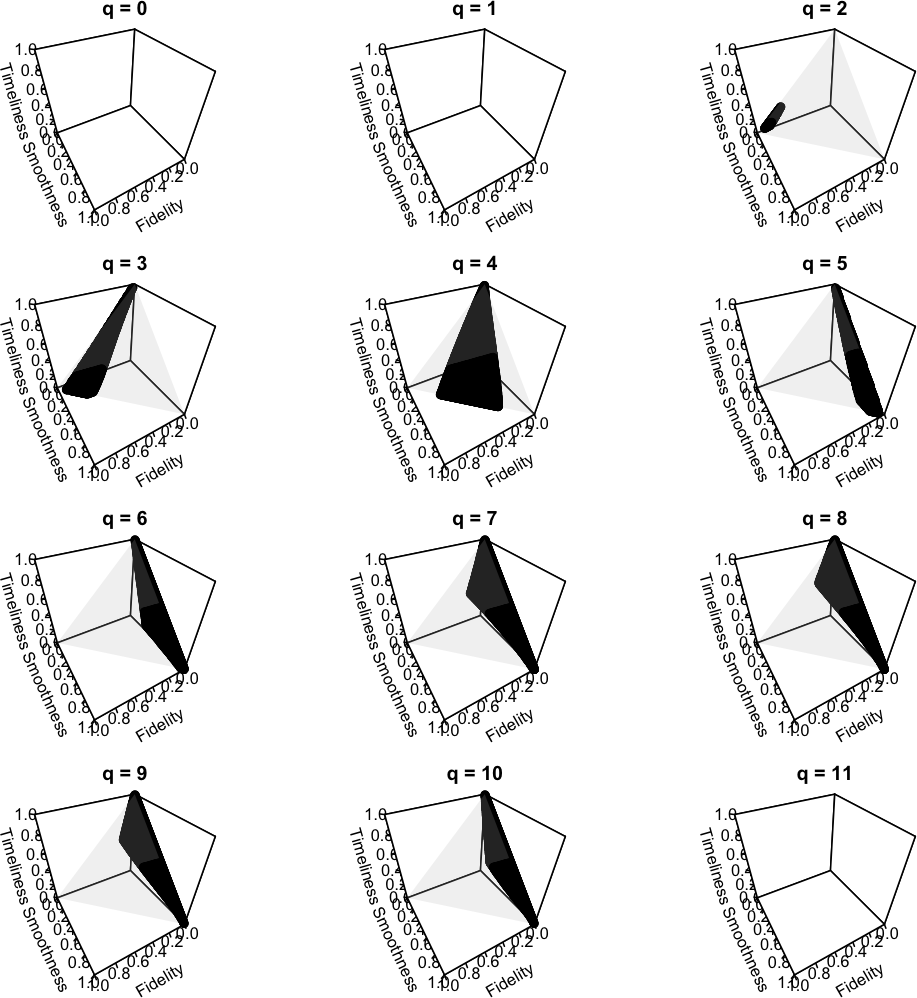
\includegraphics{img/bookdown/pdf/lc11d1-1} 

}

\caption[Ensemble des poids pour lesquels la méthode FST donne des filtres de meilleure qualité que le filtre \emph{Linear-Constant} (LC) sous contrainte de préservation des droites (\(d=1\)) et pour \(h=11\)]{Ensemble des poids pour lesquels la méthode FST donne des filtres de meilleure qualité que le filtre \emph{Linear-Constant} (LC) sous contrainte de préservation des droites (\(d=1\)) et pour \(h=11\).}\label{fig:lc11d1}

\footnotesize


\emph{Notes} : \emph{La zone grisée correspond à l'ensemble \(\left\{\begin{pmatrix}x \; y \; z \end{pmatrix}' : x+y+z=1\right\}\).}

\emph{Le graphique est vide lorsque aucun poids ne permet de trouver de filtre FST qui minimise la \emph{fidelity}, \emph{smoothness} et la \emph{timeliness} par rapport au filtre étudié.}
\normalsize\end{figure}

\newpage

\hypertarget{filtres-rkhs}{%
\subsection{Filtres RKHS}\label{filtres-rkhs}}

\begin{figure}[H]

{\centering 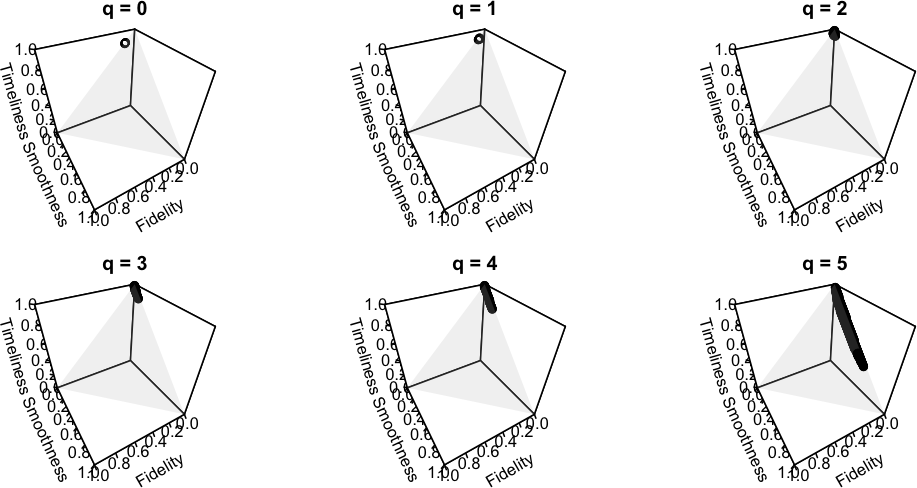
\includegraphics{img/bookdown/pdf/rkhs6d0-1} 

}

\caption[Ensemble des poids pour lesquels la méthode FST donne des filtres de meilleure qualité que le filtre \(b_{q,\varphi}\) sous contrainte de préservation des constantes (\(d=0\)) et pour \(h=6\)]{Ensemble des poids pour lesquels la méthode FST donne des filtres de meilleure qualité que le filtre \(b_{q,\varphi}\) sous contrainte de préservation des constantes (\(d=0\)) et pour \(h=6\).}\label{fig:rkhs6d0}

\footnotesize


\emph{Notes} : \emph{La zone grisée correspond à l'ensemble \(\left\{\begin{pmatrix}x \; y \; z \end{pmatrix}' : x+y+z=1\right\}\).}

\emph{Le graphique est vide lorsque aucun poids ne permet de trouver de filtre FST qui minimise la \emph{fidelity}, \emph{smoothness} et la \emph{timeliness} par rapport au filtre étudié.}
\normalsize\end{figure}

\begin{figure}[H]

{\centering 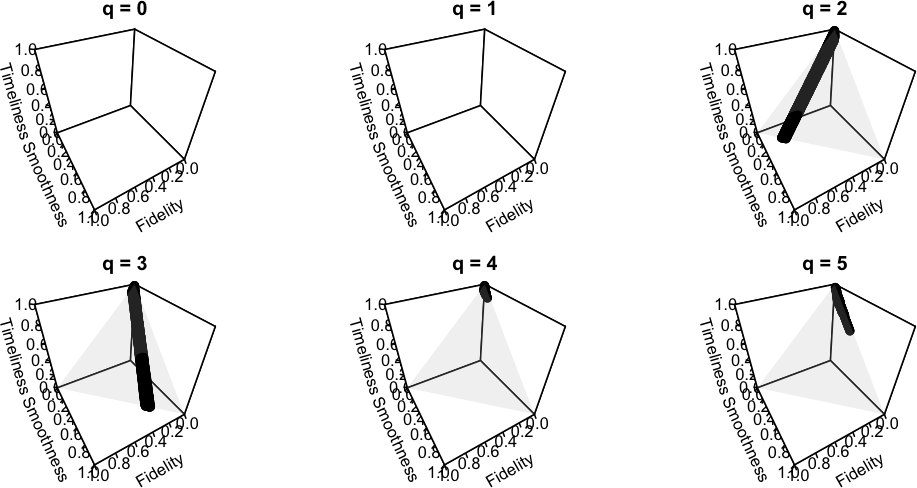
\includegraphics{img/bookdown/pdf/rkhs6d1-1} 

}

\caption[Ensemble des poids pour lesquels la méthode FST donne des filtres de meilleure qualité que le filtre \(b_{q,\varphi}\) sous contrainte de préservation des droites (\(d=1\)) et pour \(h=6\)]{Ensemble des poids pour lesquels la méthode FST donne des filtres de meilleure qualité que le filtre \(b_{q,\varphi}\) sous contrainte de préservation des droites (\(d=1\)) et pour \(h=6\).}\label{fig:rkhs6d1}

\footnotesize


\emph{Notes} : \emph{La zone grisée correspond à l'ensemble \(\left\{\begin{pmatrix}x \; y \; z \end{pmatrix}' : x+y+z=1\right\}\).}

\emph{Le graphique est vide lorsque aucun poids ne permet de trouver de filtre FST qui minimise la \emph{fidelity}, \emph{smoothness} et la \emph{timeliness} par rapport au filtre étudié.}
\normalsize\end{figure}

\begin{figure}[H]

{\centering 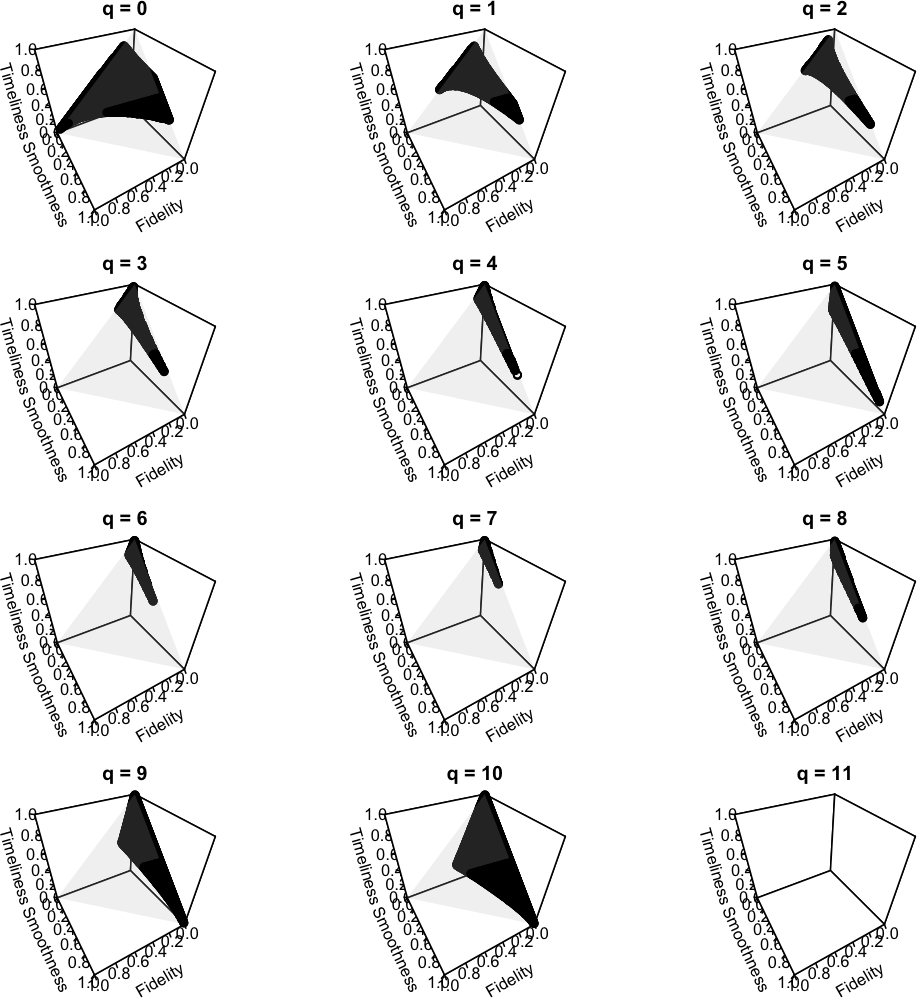
\includegraphics{img/bookdown/pdf/rkhs11d0-1} 

}

\caption[Ensemble des poids pour lesquels la méthode FST donne des filtres de meilleure qualité que le filtre \(b_{q,\varphi}\) sous contrainte de préservation des constantes (\(d=0\)) et pour \(h=11\)]{Ensemble des poids pour lesquels la méthode FST donne des filtres de meilleure qualité que le filtre \(b_{q,\varphi}\) sous contrainte de préservation des constantes (\(d=0\)) et pour \(h=11\).}\label{fig:rkhs11d0}

\footnotesize


\emph{Notes} : \emph{La zone grisée correspond à l'ensemble \(\left\{\begin{pmatrix}x \; y \; z \end{pmatrix}' : x+y+z=1\right\}\).}

\emph{Le graphique est vide lorsque aucun poids ne permet de trouver de filtre FST qui minimise la \emph{fidelity}, \emph{smoothness} et la \emph{timeliness} par rapport au filtre étudié.}
\normalsize\end{figure}

\begin{figure}[H]

{\centering 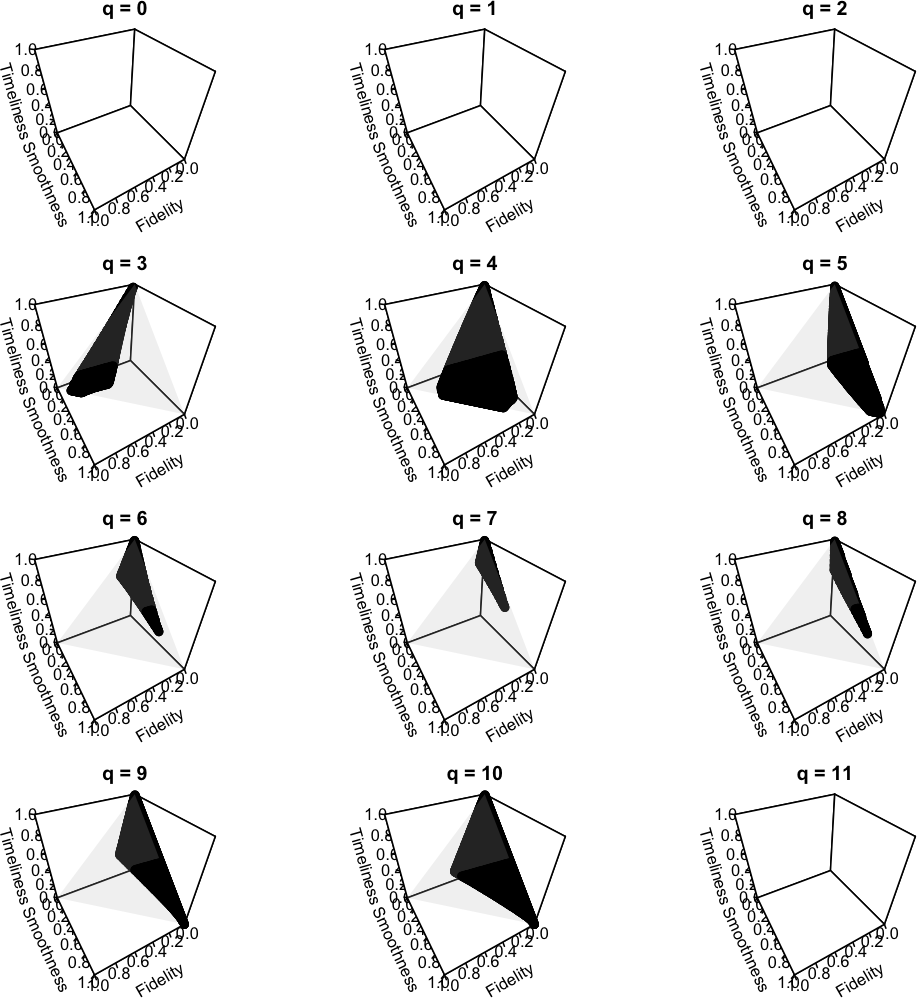
\includegraphics{img/bookdown/pdf/rkhs11d1-1} 

}

\caption[Ensemble des poids pour lesquels la méthode FST donne des filtres de meilleure qualité que le filtre \(b_{q,\varphi}\) sous contrainte de préservation des droites (\(d=1\)) et pour \(h=11\)]{Ensemble des poids pour lesquels la méthode FST donne des filtres de meilleure qualité que le filtre \(b_{q,\varphi}\) sous contrainte de préservation des droites (\(d=1\)) et pour \(h=11\).}\label{fig:rkhs11d1}

\footnotesize


\emph{Notes} : \emph{La zone grisée correspond à l'ensemble \(\left\{\begin{pmatrix}x \; y \; z \end{pmatrix}' : x+y+z=1\right\}\).}

\emph{Le graphique est vide lorsque aucun poids ne permet de trouver de filtre FST qui minimise la \emph{fidelity}, \emph{smoothness} et la \emph{timeliness} par rapport au filtre étudié.}
\normalsize\end{figure}

\newpage

\hypertarget{an-x11}{%
\section{Décomposition avec X-13ARIMA}\label{an-x11}}

Pour décomposer une série, l'algorithme X-13-ARIMA (et TRAMO-SEATS) fonctionnent en deux grandes étapes :

\begin{enumerate}
\def\labelenumi{\arabic{enumi}.}
\item
  Dans la première étape, la série est corrigée des jours ouvrables et des points atypiques à l'aide d'un modèle ARIMA. La série initiale est également prolongée par prévision sur la dernière année pour la seconde étape.
  La série corrigée et prolongée est appelée série \emph{linéarisée}.
\item
  Dans une seconde étape, cette série linéarisée, notée \(X_t\) est décomposée en trois composantes saisonnalité \(S_t\), tendance-cycle \(TC_t\) et irrégulier \(I_t\).
\end{enumerate}

Dans ce rapport nous nous intéressons essentiellement à cette seconde étape, où la méthode utilisée pour extraire la composante tendance-cycle en fin de période sera modifiée.
La méthode de décomposition utilisée dans X-13ARIMA, similaire à celle de X-11, est détaillée de manière très précise dans \textcite{ladiray1999comprendre}.
Cette annexe reprend de manière synthétique la description faite dans cet article.

Pour la décomposition l'algorithme estime itérativement les différentes composantes en appliquant des moyennes mobiles.
Cette algorithme peut se décomposer en l'application de deux blocs successifs.
Pour une série mensuelle et dans le cadre d'une décomposition dite additive (\(X_t=S_t+TC_t+I_t\))\footnote{
  D'autres schémas de décomposition peuvent être considérés, par exemple une décomposition multiplicative : \(X_t=S_t\times TC_t\times I_t\).} :

\begin{enumerate}
\def\labelenumi{\arabic{enumi}.}
\item
  Estimation de la tendance-cycle par une moyenne mobile \(M_{2\times 12}\).
  C'est une moyenne mobile symétrique qui conserve les tendances linéaires et supprime la saisonnalité (elle est calculée en composant les deux moyennes mobiles simples \(1/12(B^6+B^5+\dots+B^{-5})\) et \(1/12(B^5+B^4+\dots+B^{-6})\)).
  À cette étape aucune moyenne mobile asymétrique n'est utilisée, les 6 premiers points et les 6 derniers points ne sont donc pas calculés.
  \[
  TC_t^{(1)}=M_{2\times 12}(X_t)
  \]
\item
  Estimation de la composante saisonnier-irrégulier :
  \[
  (S_t+I_t)^{(1)}= X_t - TC_t^{(1)}
  \]
\item
  Estimation de la composante saisonnière par moyenne mobile \(M_{3\times 3}\) (composition de deux moyennes mobiles symétriques simples de 3 termes \(1/3(B+I+B^{-1})\)) appliquée chaque mois de manière indépendante.
  En fin de période, des moyennes mobiles asymétriques spécifiques sont utilisées :
  \[
  S_t^{(1)}= M_{3\times 3}\left[(S_t+I_t)^{(1)}\right]
  \]
  Puis une normalisation est faite entre les mois :
  \[
  Snorm_t^{(1)}= S_t^{(1)} - M_{2\times 12}\left(S_t^{(1)}\right)
  \]
  En fin de série, la moyenne mobile \(M_{2\times 12}\left(S_t^{(1)}\right)\) ne pouvant être calculée sur les 6 derniers mois, la dernière valeur calculée de \(M_{2\times 12}\left(S_t^{(1)}\right)\) est prolongée sur les 6 derniers mois (et inversement pour le début de période).
  Les coefficients saisonniers manquants (du fait de la première estimation de la tendance-cycle à l'étape 1) sont imputés en utilisant la valeur la plus proche du mois considéré.
\item
  Estimation de la série corrigée des variations saisonnières :
  \[
  Xsa_t^{(1)}= (TC_t+I_t)^{(1)} = X_t - Snorm_t^{(1)}
  \]
\end{enumerate}

Ensuite, les mêmes étapes sont répétées mais en faisant l'estimation de la tendance-cycle sur la série désaisonnalisée.
Cela permet notamment d'utiliser des moyennes mobiles ayant de meilleurs propriétés en termes de préservation polynomiale (celles notamment présentées dans ce rapport) mais qui ne supprime pas la saisonnalité.

\begin{enumerate}
\def\labelenumi{\arabic{enumi}.}
\setcounter{enumi}{4}
\item
  Estimation de la tendance-cycle par moyenne de Henderson.
  L'ordre de la moyenne mobile est déterminée de automatiquement, à partir de l'I-C ratio, entre une moyenne centrée de 9 termes (\(h=4\)), 13 termes (\(h=6\), c'est ce qui est retenu dans la majorité des cas) et 23 termes (\(h=11\)).
  En fin de période, des moyennes mobiles asymétriques de Musgrave sont utilisées.
  C'est à cette étape que dans nos différentes simulations nous modifions les filtres asymétriques utilisés en ne prenant pas en compte les prévisions de la série linéarisée.
  \[
  TC_t^{(2)}=H_{13}(Xsa_t^{(1)})
  \]
\item
  Estimation de la composante saisonnier-irrégulier :
  \[
  (S_t+I_t)^{(2)}= X_t - TC_t^{(2)}
  \]
\item
  Estimation de la composante saisonnière par moyenne mobile dont l'ordre est détectée automatiquement entre une moyenne mobile \(M_{3\times 3}\), \(M_{3\times 5}\) (ce qui est généralement retenu) et \(M_{3\times 7}\).
  Sur chaque mois :
  \[
  S_t^{(2)}= M_{3\times 5}\left[(S_t+I_t)^{(2)}\right]
  \]
  Puis une normalisation est faite (avec même traitement en fin de période qu'à l'étape 3) :
  \[
  Snorm_t^{(2)}=S_t^{(2)} - M_{2\times 12}\left(S_t^{(2)}\right)
  \]
\item
  Estimation de la série corrigée des variations saisonnières :
  \[
  Xsa_t^{(2)}= (TC_t+I_t)^{(2)} = X_t - Snorm_t^{(2)}
  \]
\end{enumerate}

L'étape 5 est répétée une dernière fois sur cette série désaisonnalisée afin d'avoir l'estimation finale de la tendance-cycle.

Les moyennes mobiles étant très sensibles à la présence de points atypiques, une correction automatique de l'irrégulier est effectuée, à partir de \(S_t+I_t\), avant les étapes 3 et 7 :

\begin{itemize}
\item
  Une première estimation de \(S_t\) et donc de \(I_t\) (par soustraction) est effectuée de la même façon qu'aux étapes 3 et 7.
\item
  Ensuite, pour chaque année, un écart-type mobile de l'irrégulier, noté \(\sigma\), est calculé sur 5 ans, l'année étudiée étant l'année centrale (pour les deux dernières années, l'écart-type de l'antépénultième année est considérée).
\item
  On affecte, à chaque valeur de \(I_t\), un poids \(p_t\) en fonction de son écart à l'écart-type associé (voir graphique \ref{fig:correctionautox11}) :

  \begin{itemize}
  \item
    si \(\lvert I_t\rvert\leq 1,5 \sigma\) un poids de 1 est affecté à la date \(t\) (i.e.; le point n'est pas considéré comme atypique) ;
  \item
    si \(\lvert I_t\rvert\geq 2,5 \sigma\), un poids de 0 est affecté à la date \(t\) ;
  \item
    si \(1,5 \sigma<\lvert I_t\rvert< 2,5 \sigma\), un poids variant linéairement entre 0 et 1 est affecté à la date \(t\).
  \end{itemize}
\end{itemize}

Les seuils de 1,5 et de 2,5 peuvent être modifiés par l'utilisateur.

\begin{figure}

{\centering 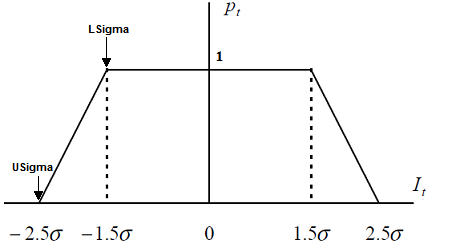
\includegraphics[width=1\linewidth]{img/correction_auto_X11} 

}

\caption[Poids utilisés par X-13ARIMA pour la correction de l'irrégulier]{Poids utilisés par X-13ARIMA pour la correction de l'irrégulier.}\label{fig:correctionautox11}

\footnotesize
\normalsize\end{figure}

\begin{itemize}
\tightlist
\item
  Enfin, pour chaque date pour laquelle l'irrégulier n'a pas un poids de 1, \((S+I)_t\) est remplacée par une moyenne pondérée de 5 valeurs : la valeur à la date \(t\) avec un poids \(p_t\) et les deux valeurs précédentes et suivantes, pour le même mois, ayant une pondération de 1.
  En fin de période, la moyenne pondérée est calculée à partir de l'observation courante et les quatre valeurs les plus proches du même mois ayant une pondération de 1.
\end{itemize}

\newpage

\hypertarget{an-plotseries}{%
\section{Exemples d'estimations de la tendance-cycle}\label{an-plotseries}}

\begin{figure}[H]

{\centering 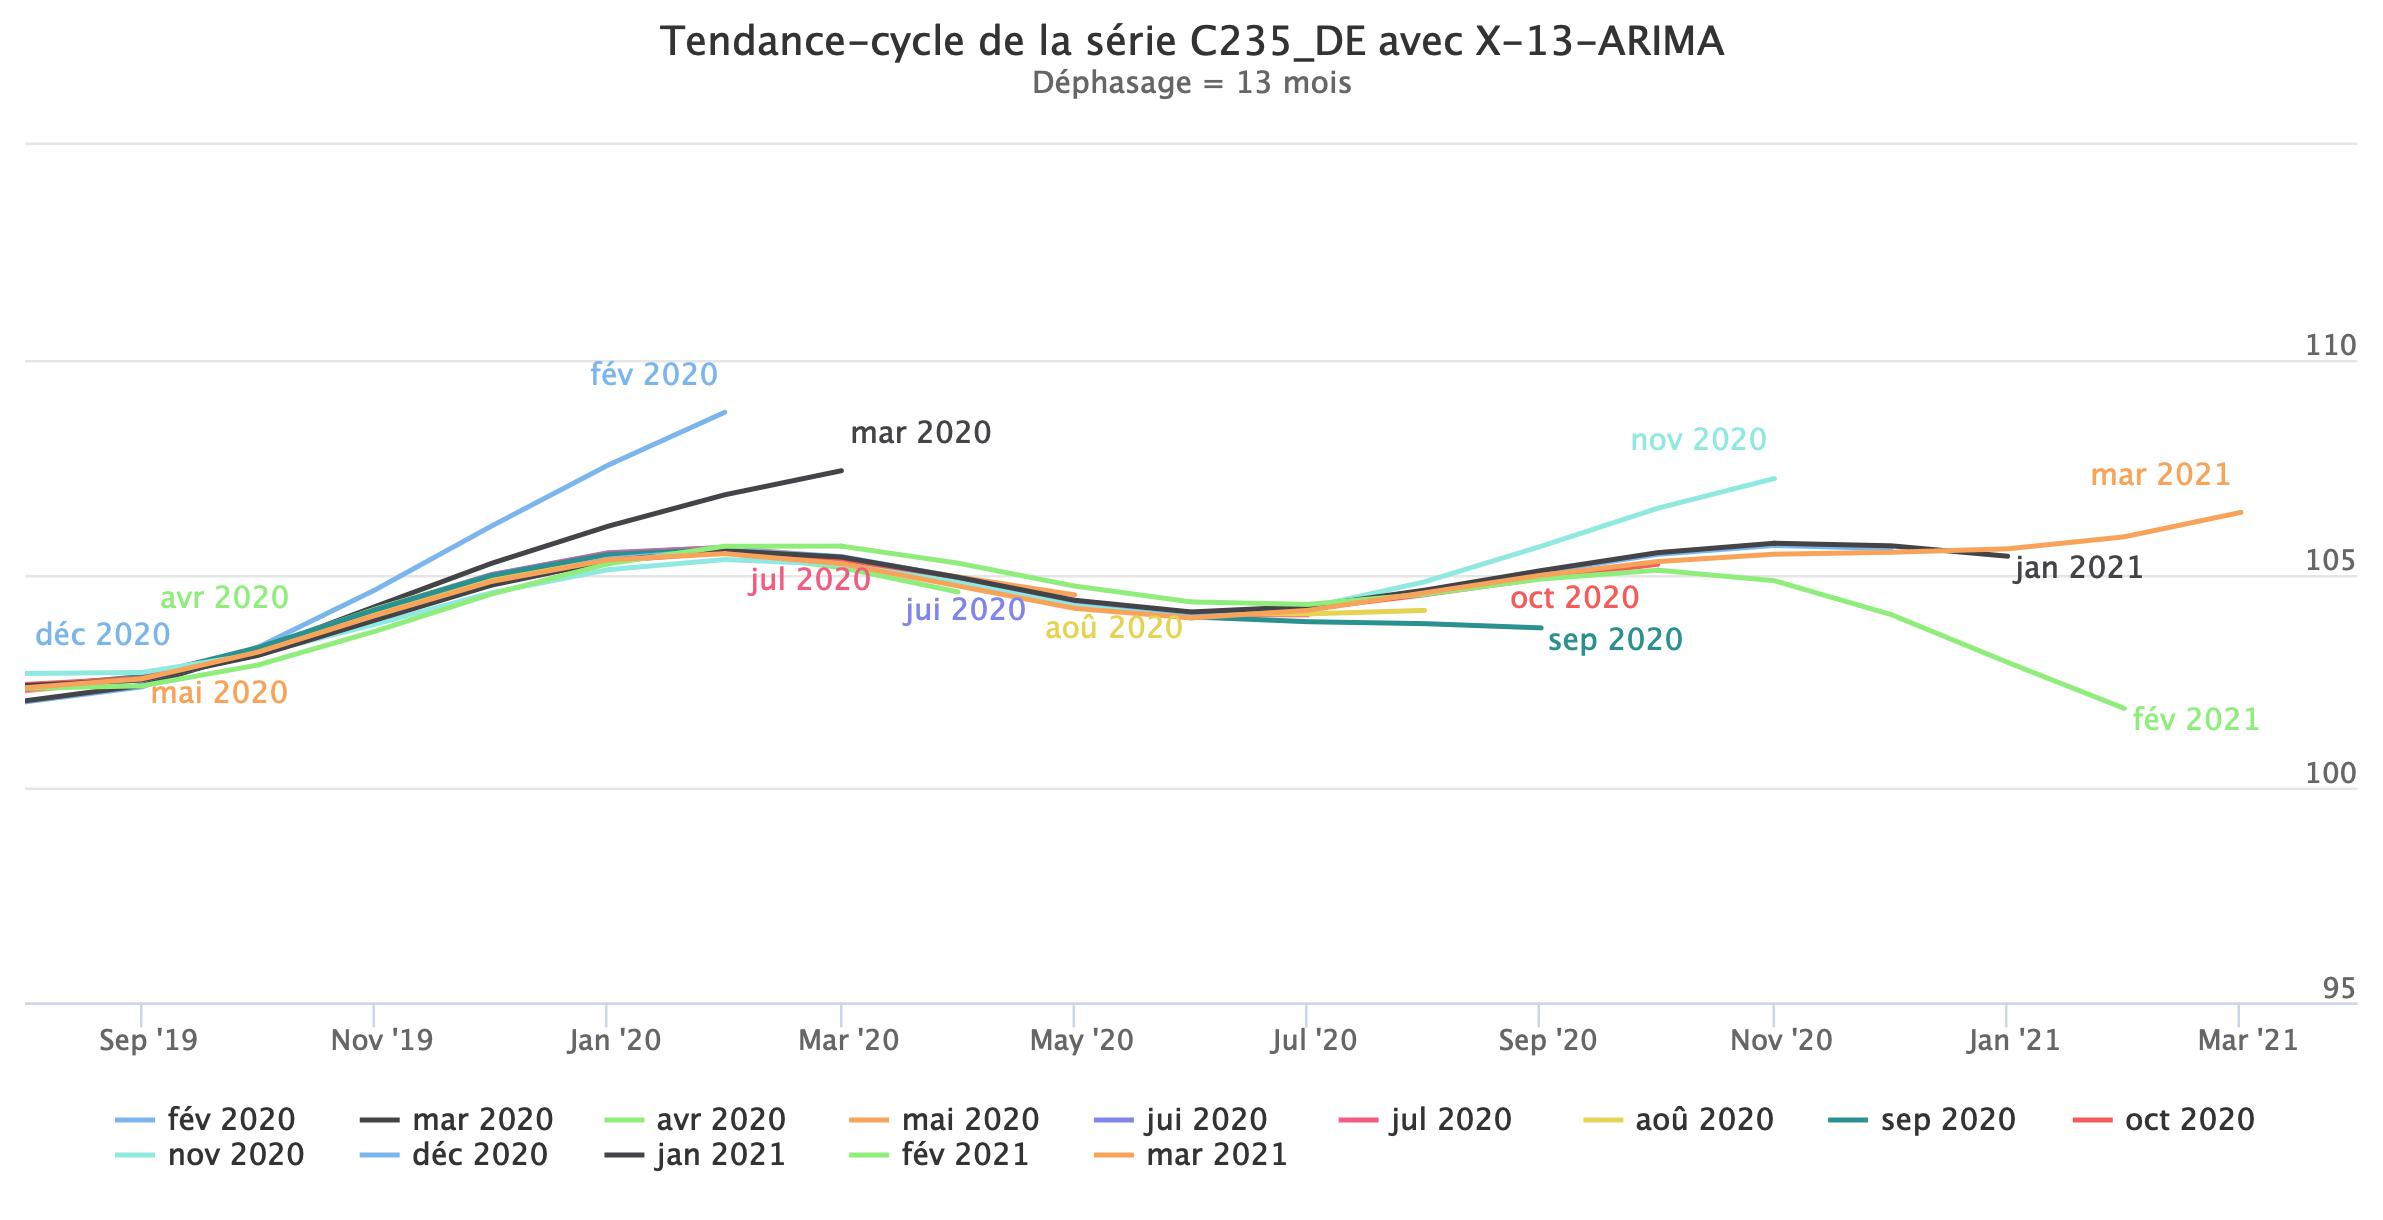
\includegraphics[width=0.9\linewidth,]{img/simulations/c235_de_x13} 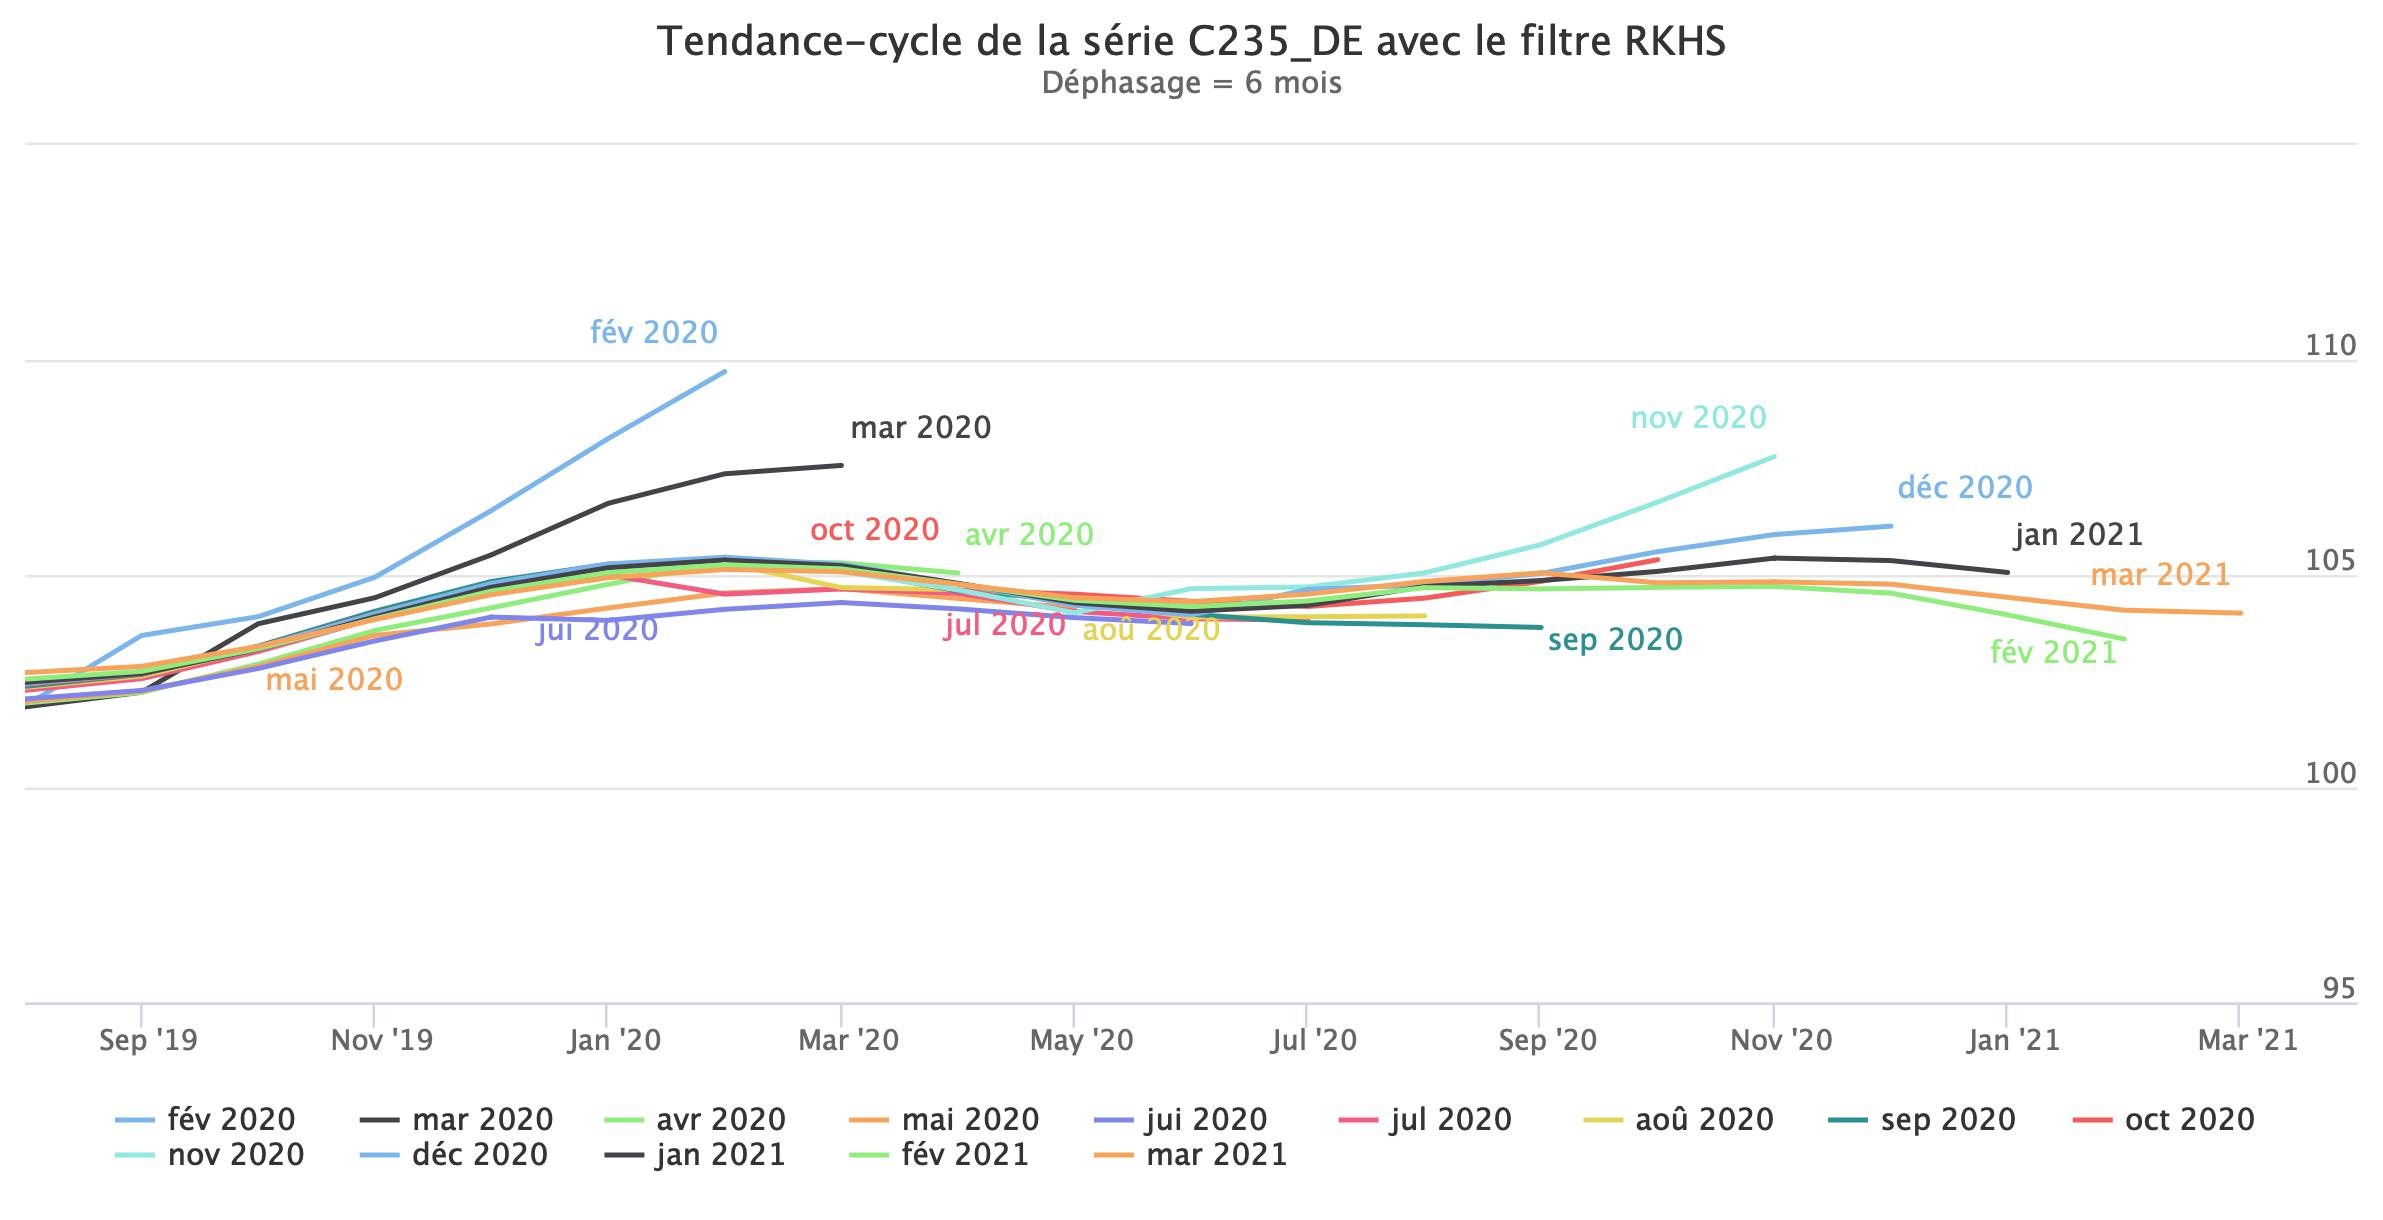
\includegraphics[width=0.9\linewidth,]{img/simulations/c235_de_rkhs_timeliness} 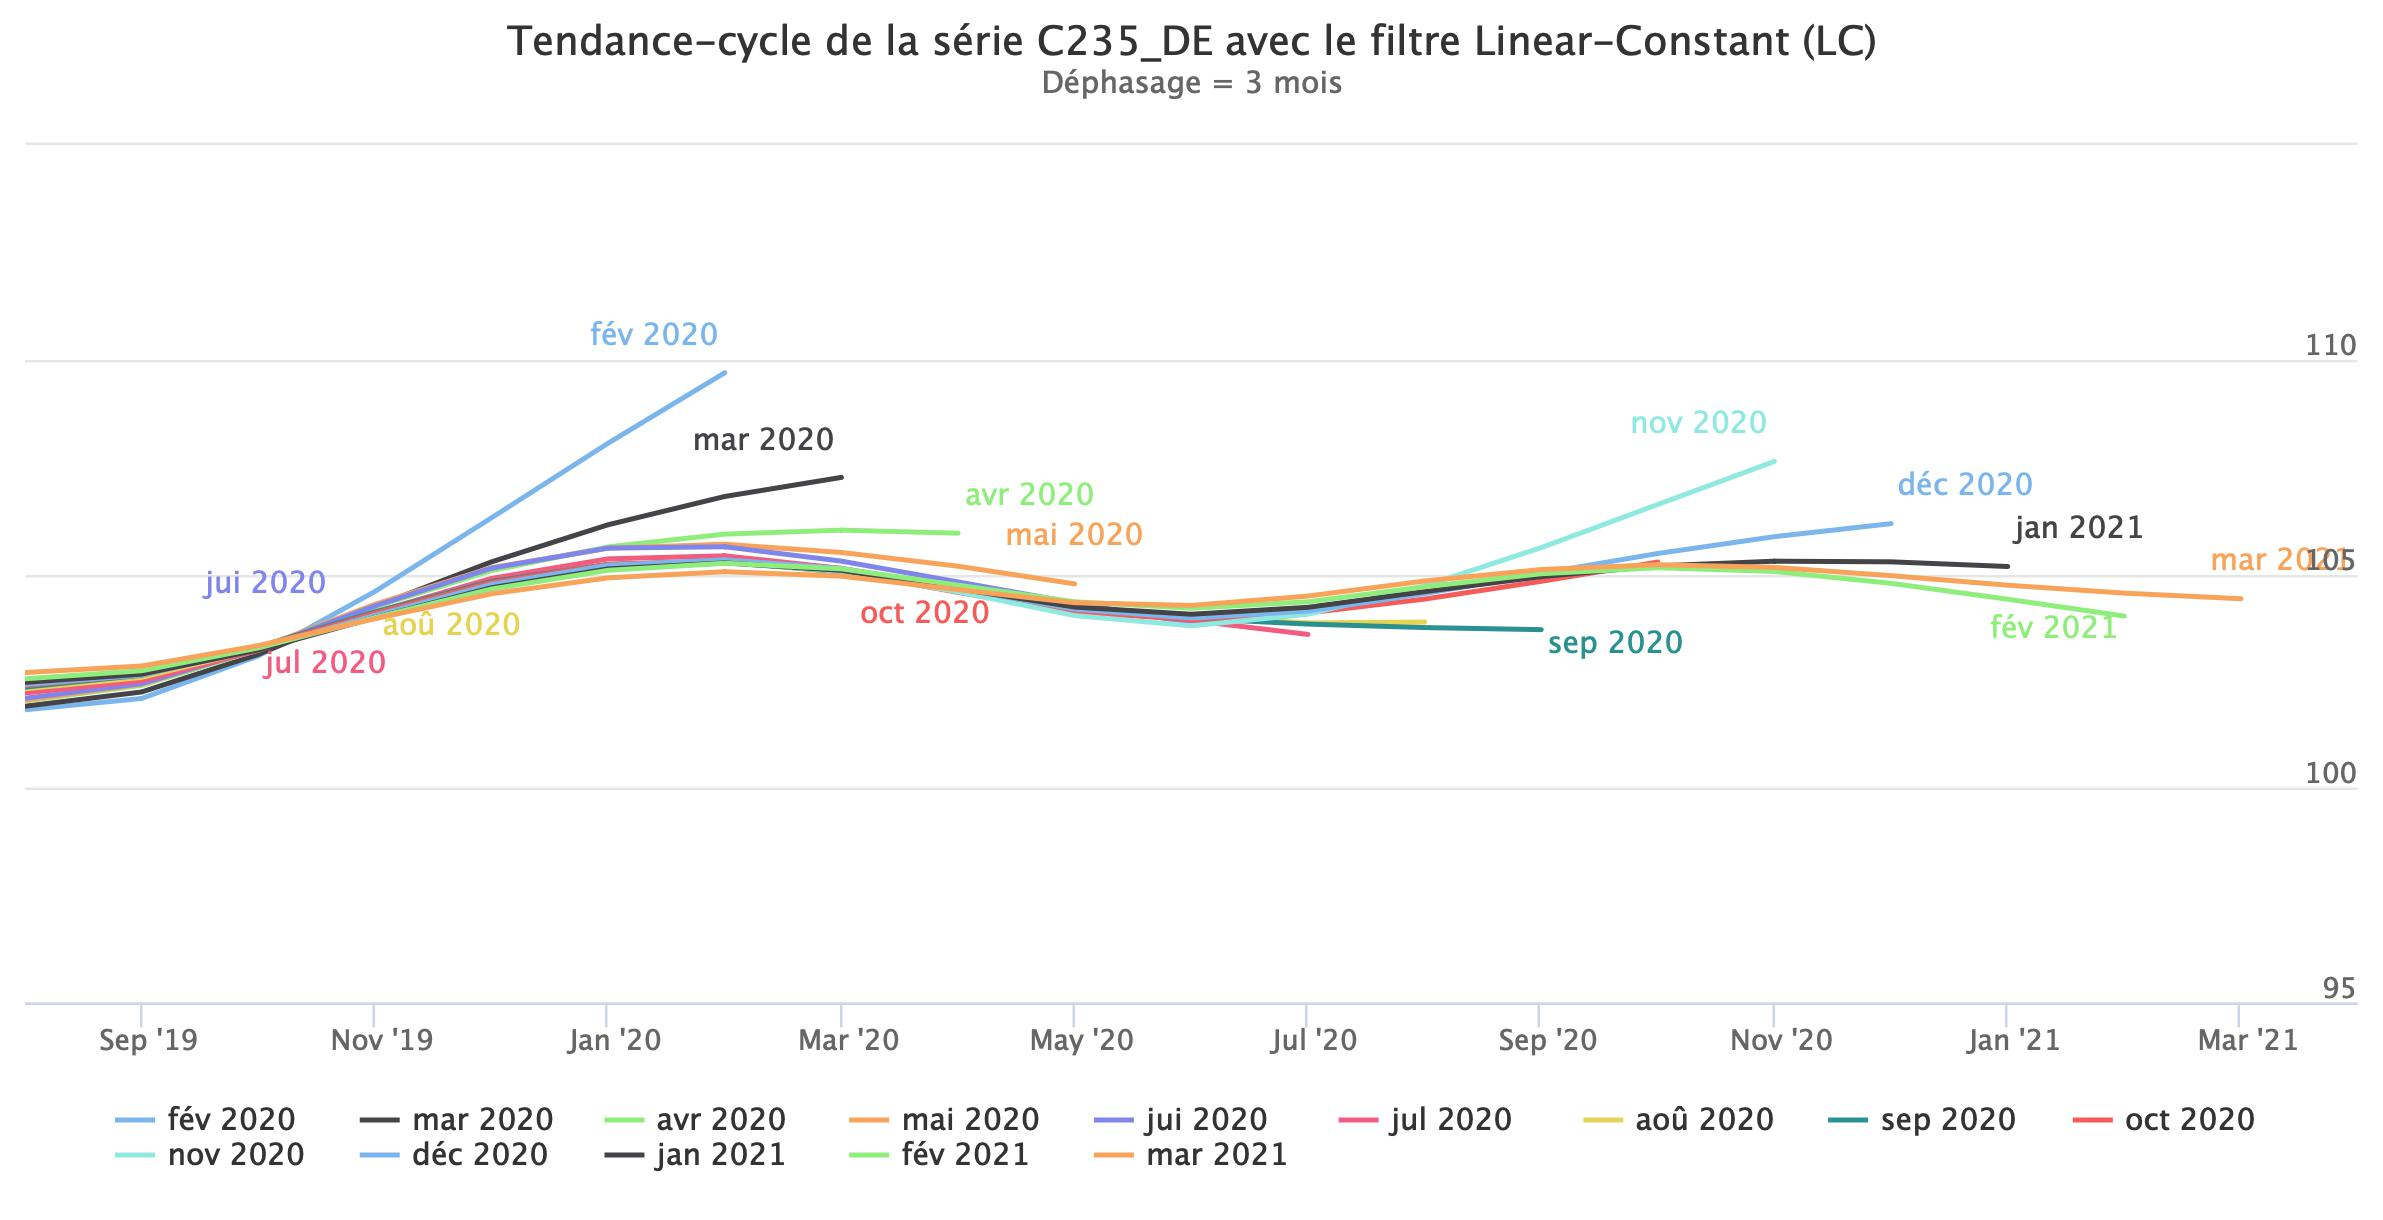
\includegraphics[width=0.9\linewidth,]{img/simulations/c235_de_lc} 

}

\caption[Estimations de la tendance-cycle pour l'indice de production industriel dans la fabrication de ciment, chaux et plâtre (C235) en Allemagne (point de retournement en février 2020)]{Estimations de la tendance-cycle pour l'indice de production industriel dans la fabrication de ciment, chaux et plâtre (C235) en Allemagne (point de retournement en février 2020).}\label{fig:c235dep1}

\footnotesize
\normalsize\end{figure}

\begin{figure}[H]

{\centering 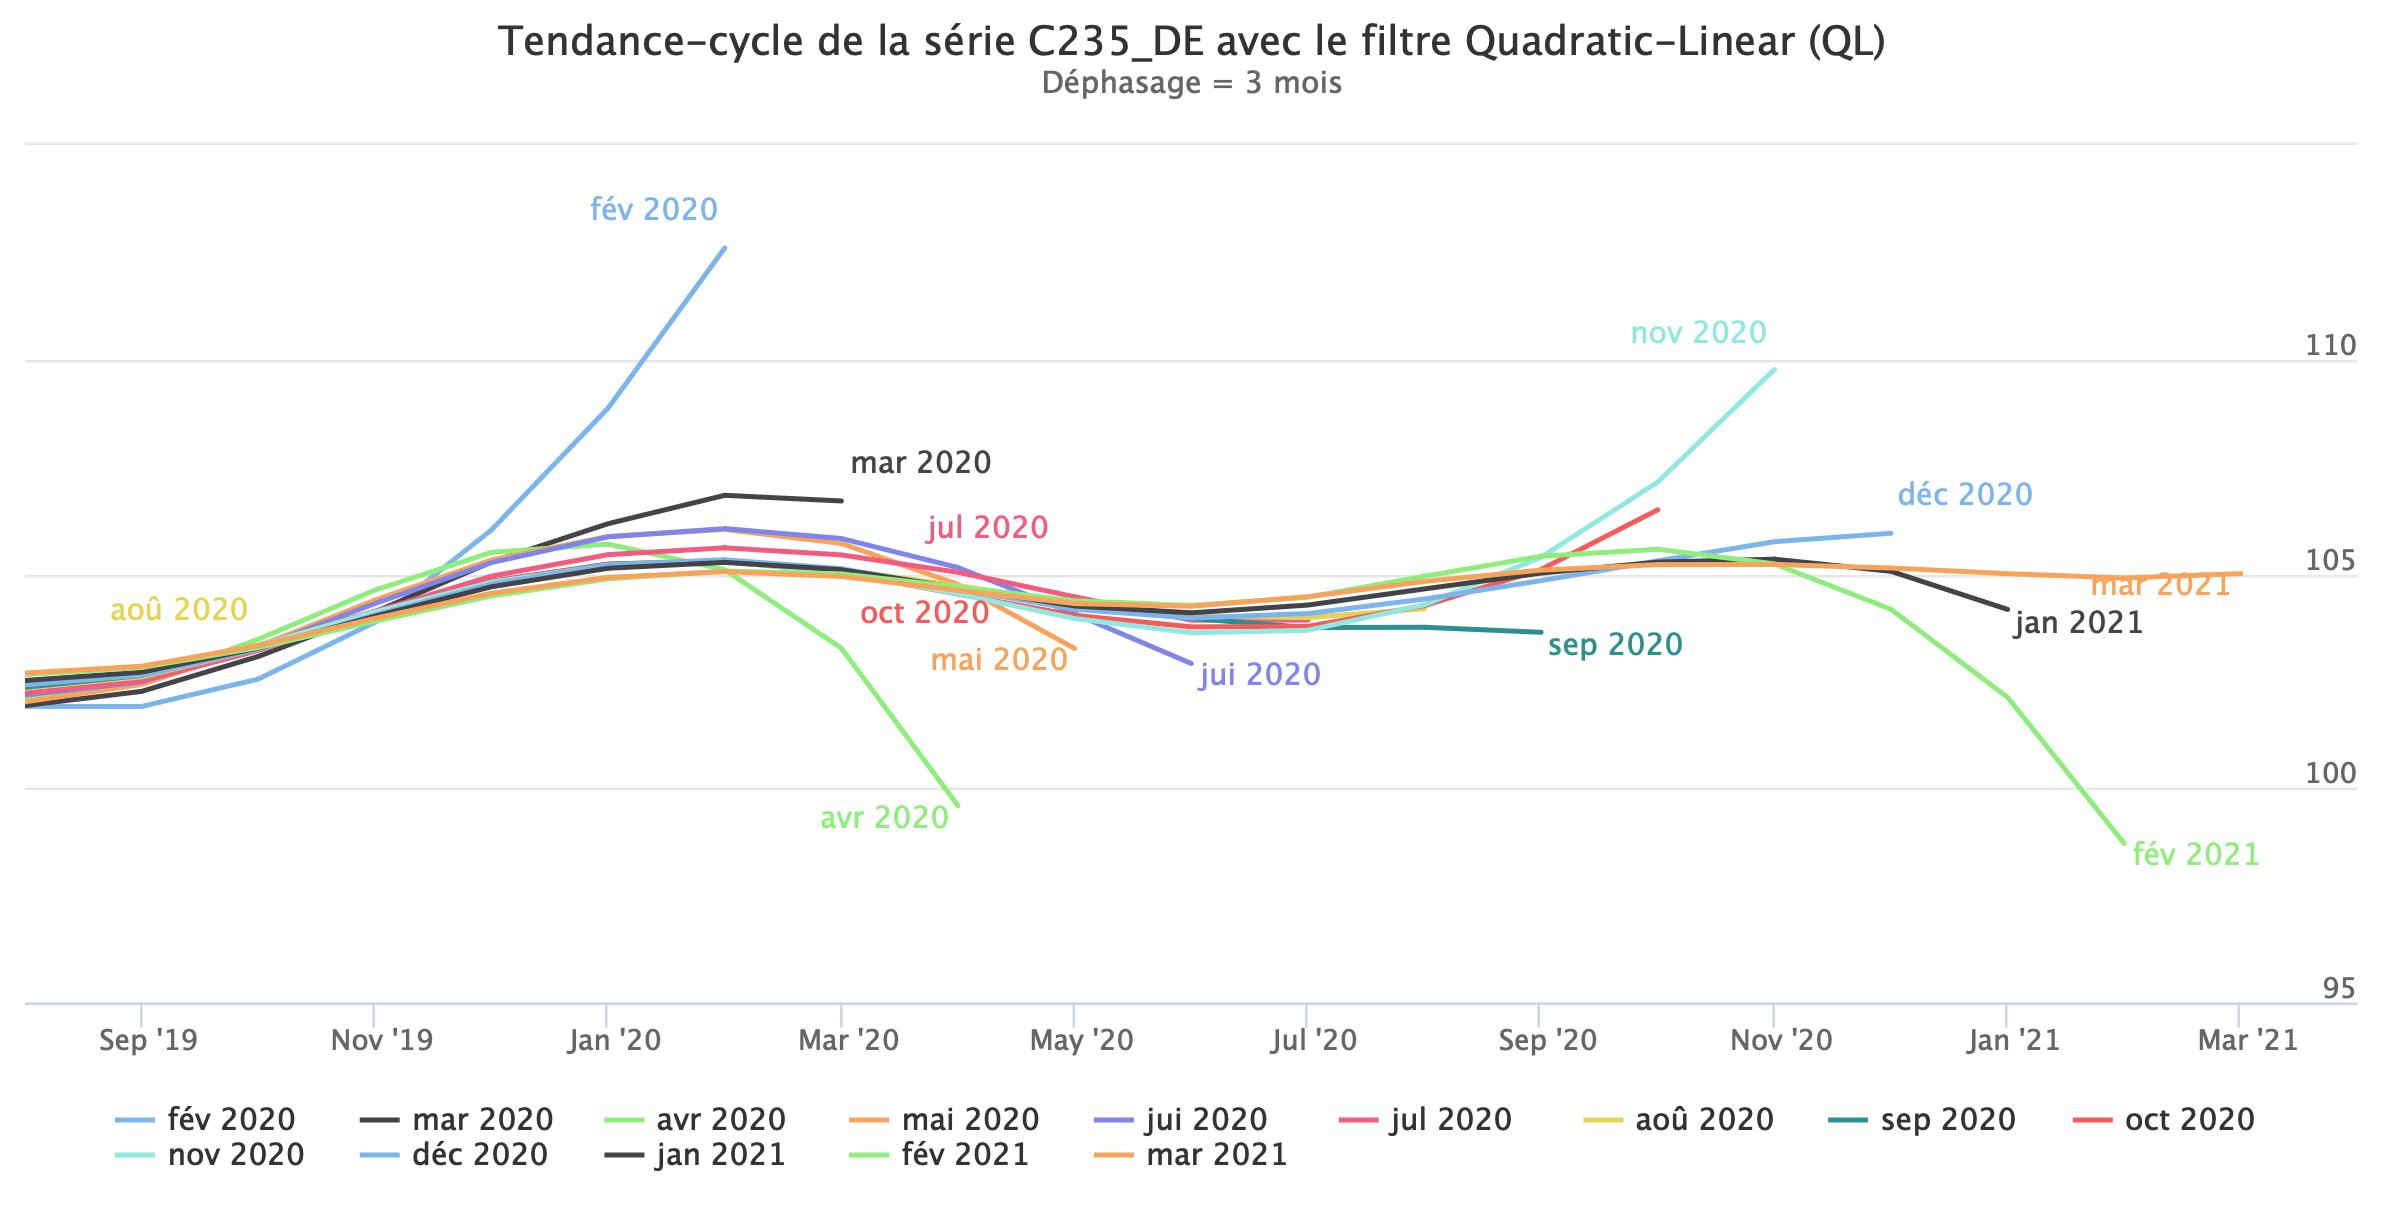
\includegraphics[width=0.9\linewidth,]{img/simulations/c235_de_ql} 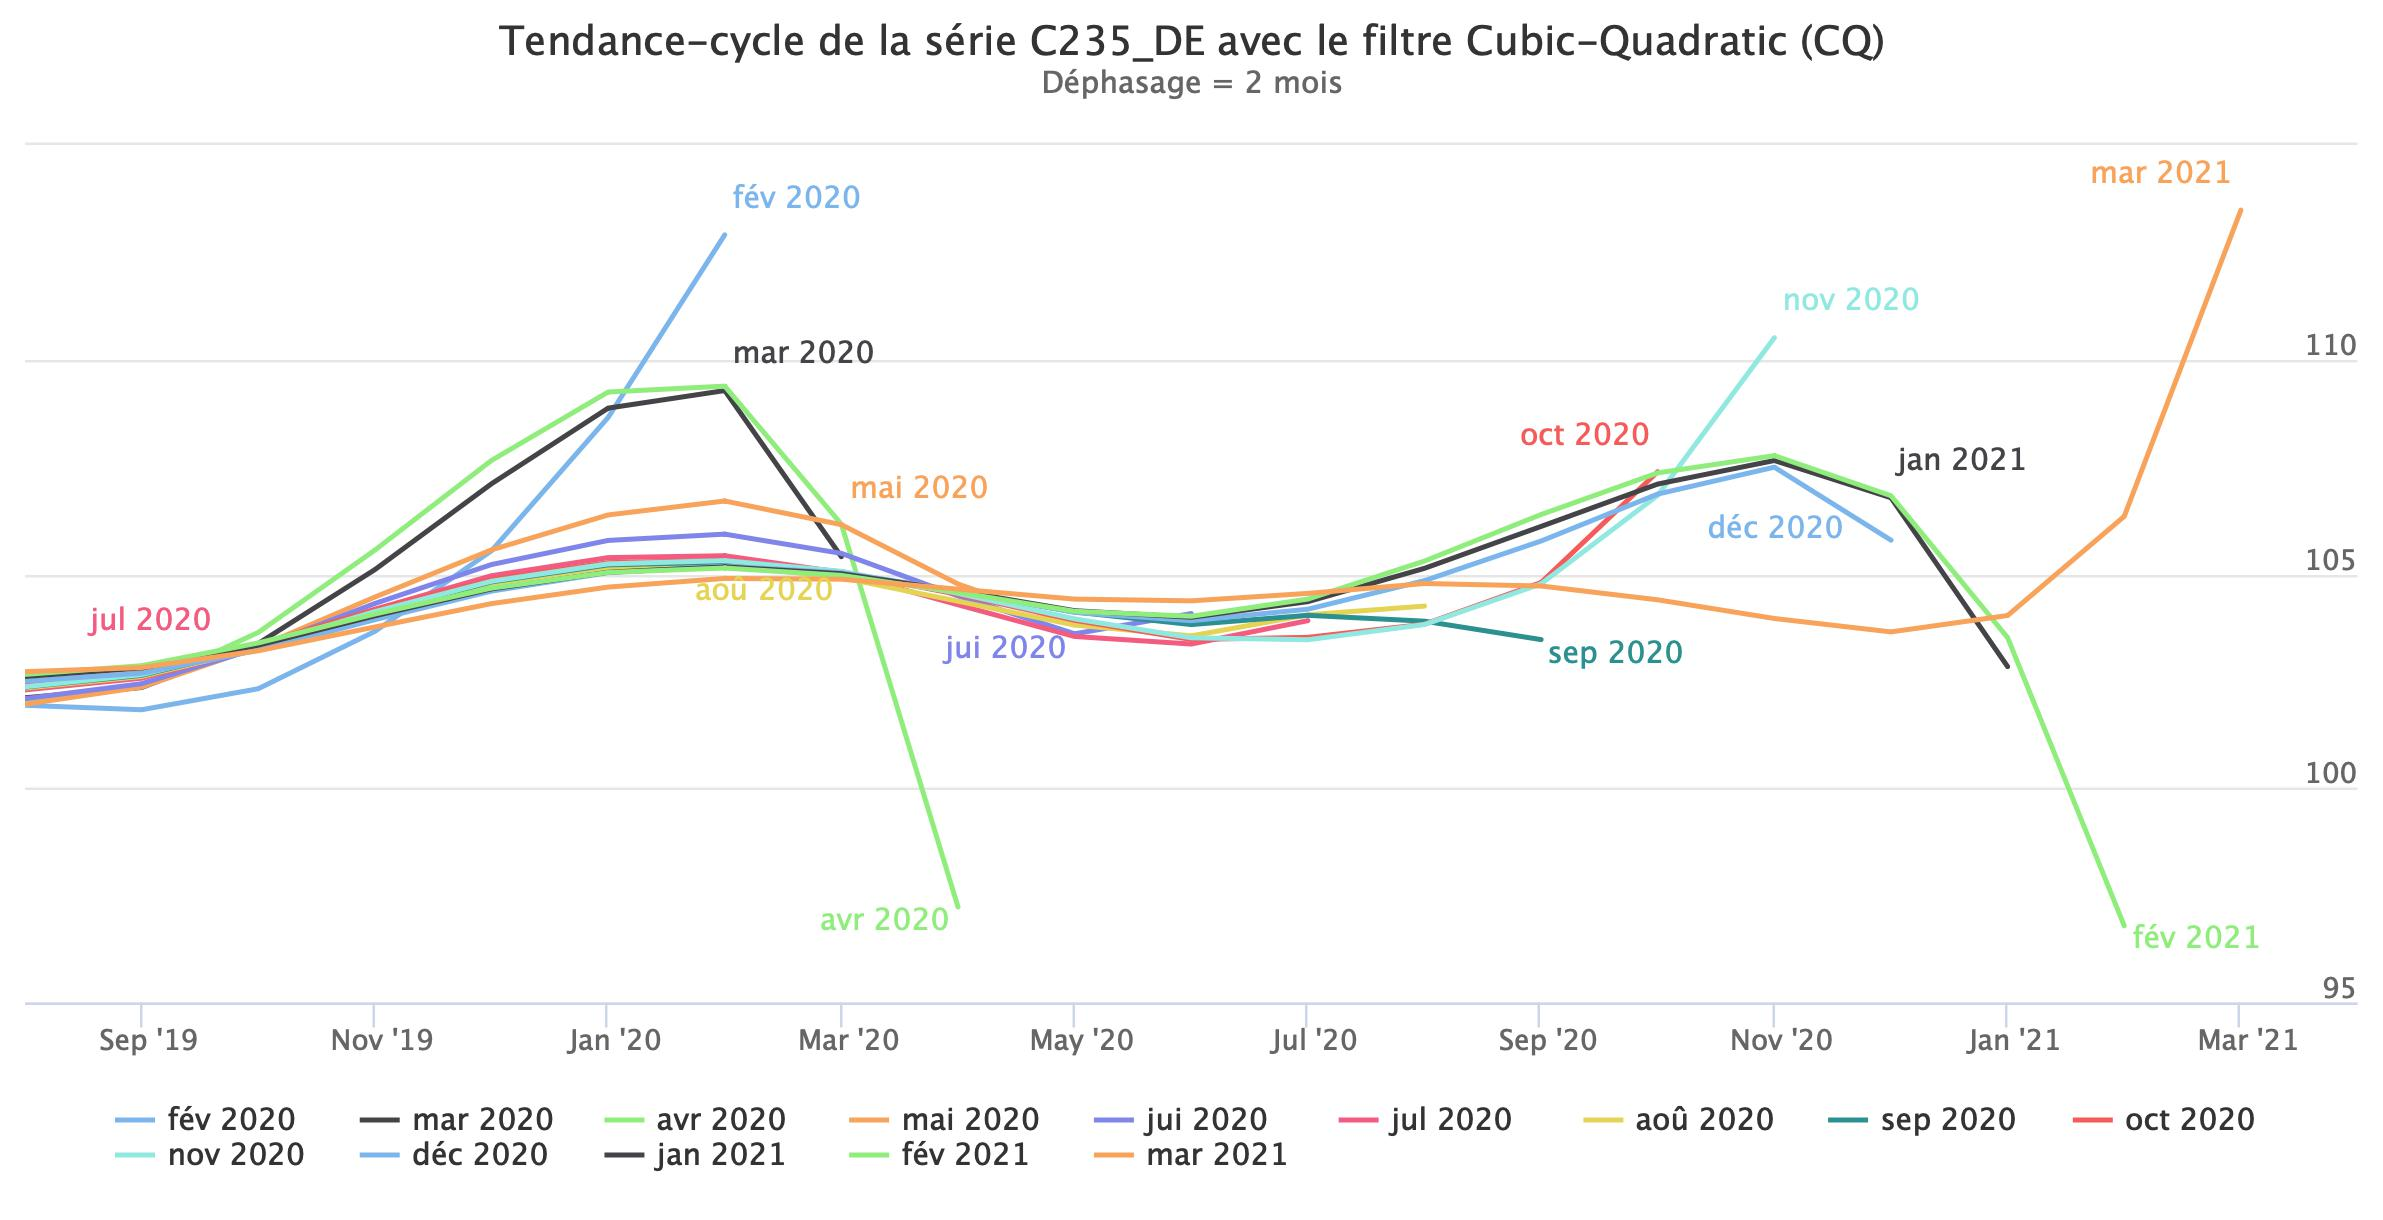
\includegraphics[width=0.9\linewidth,]{img/simulations/c235_de_cq} 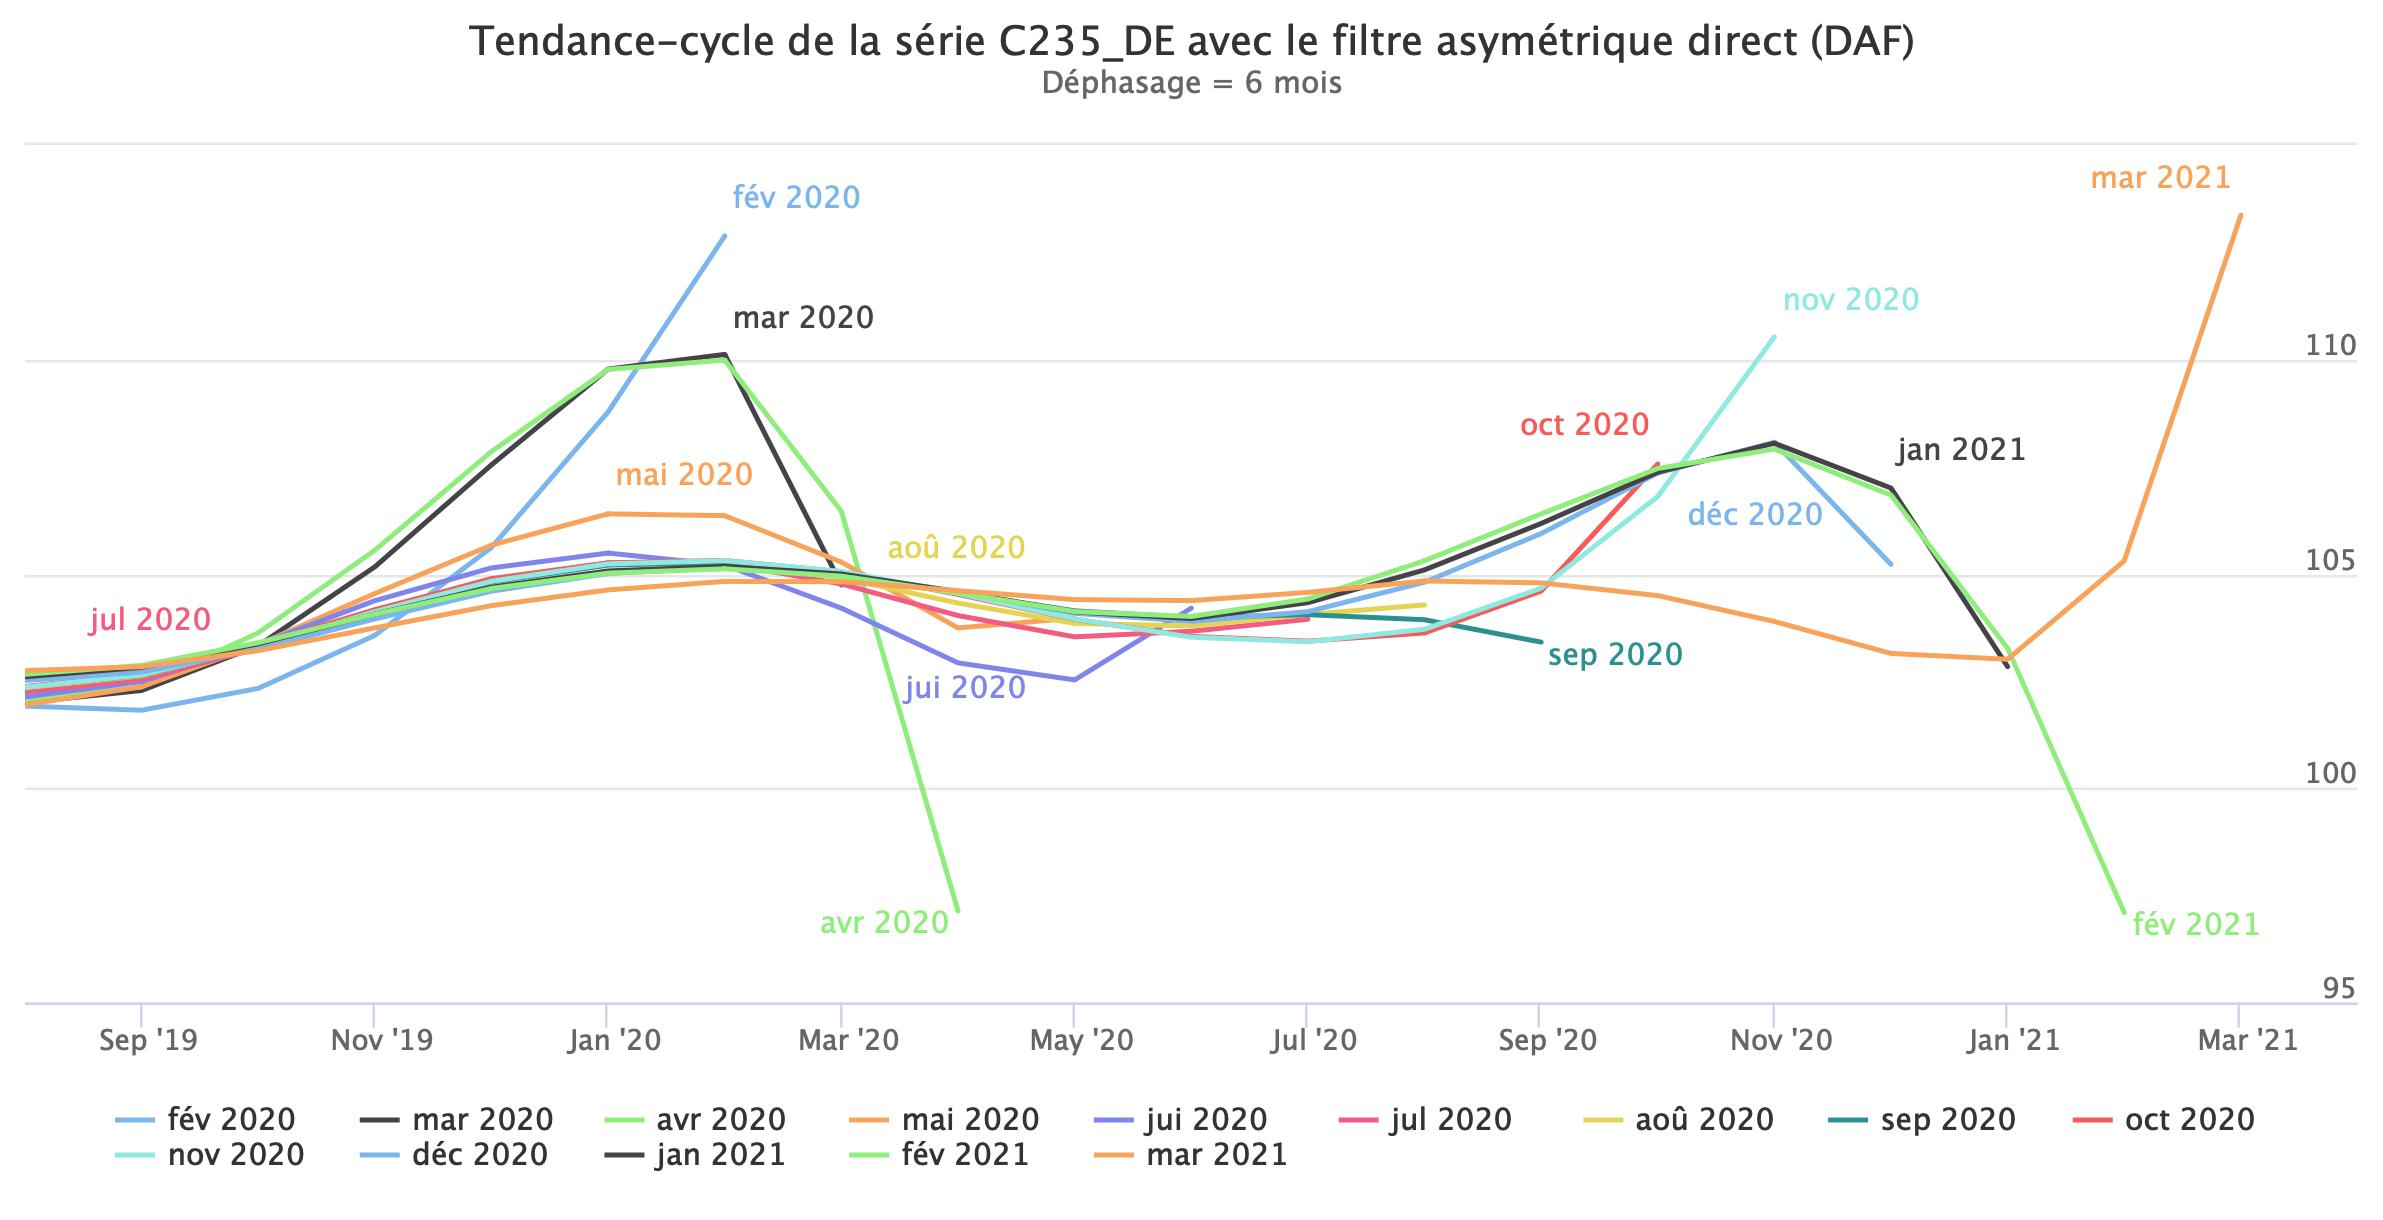
\includegraphics[width=0.9\linewidth,]{img/simulations/c235_de_daf} 

}

\caption[Estimations de la tendance-cycle pour l'indice de production industriel dans la fabrication de ciment, chaux et plâtre (C235) en Allemagne (point de retournement en février 2020)]{Estimations de la tendance-cycle pour l'indice de production industriel dans la fabrication de ciment, chaux et plâtre (C235) en Allemagne (point de retournement en février 2020).}\label{fig:c235dep2}

\footnotesize
\normalsize\end{figure}

\begin{figure}[H]

{\centering 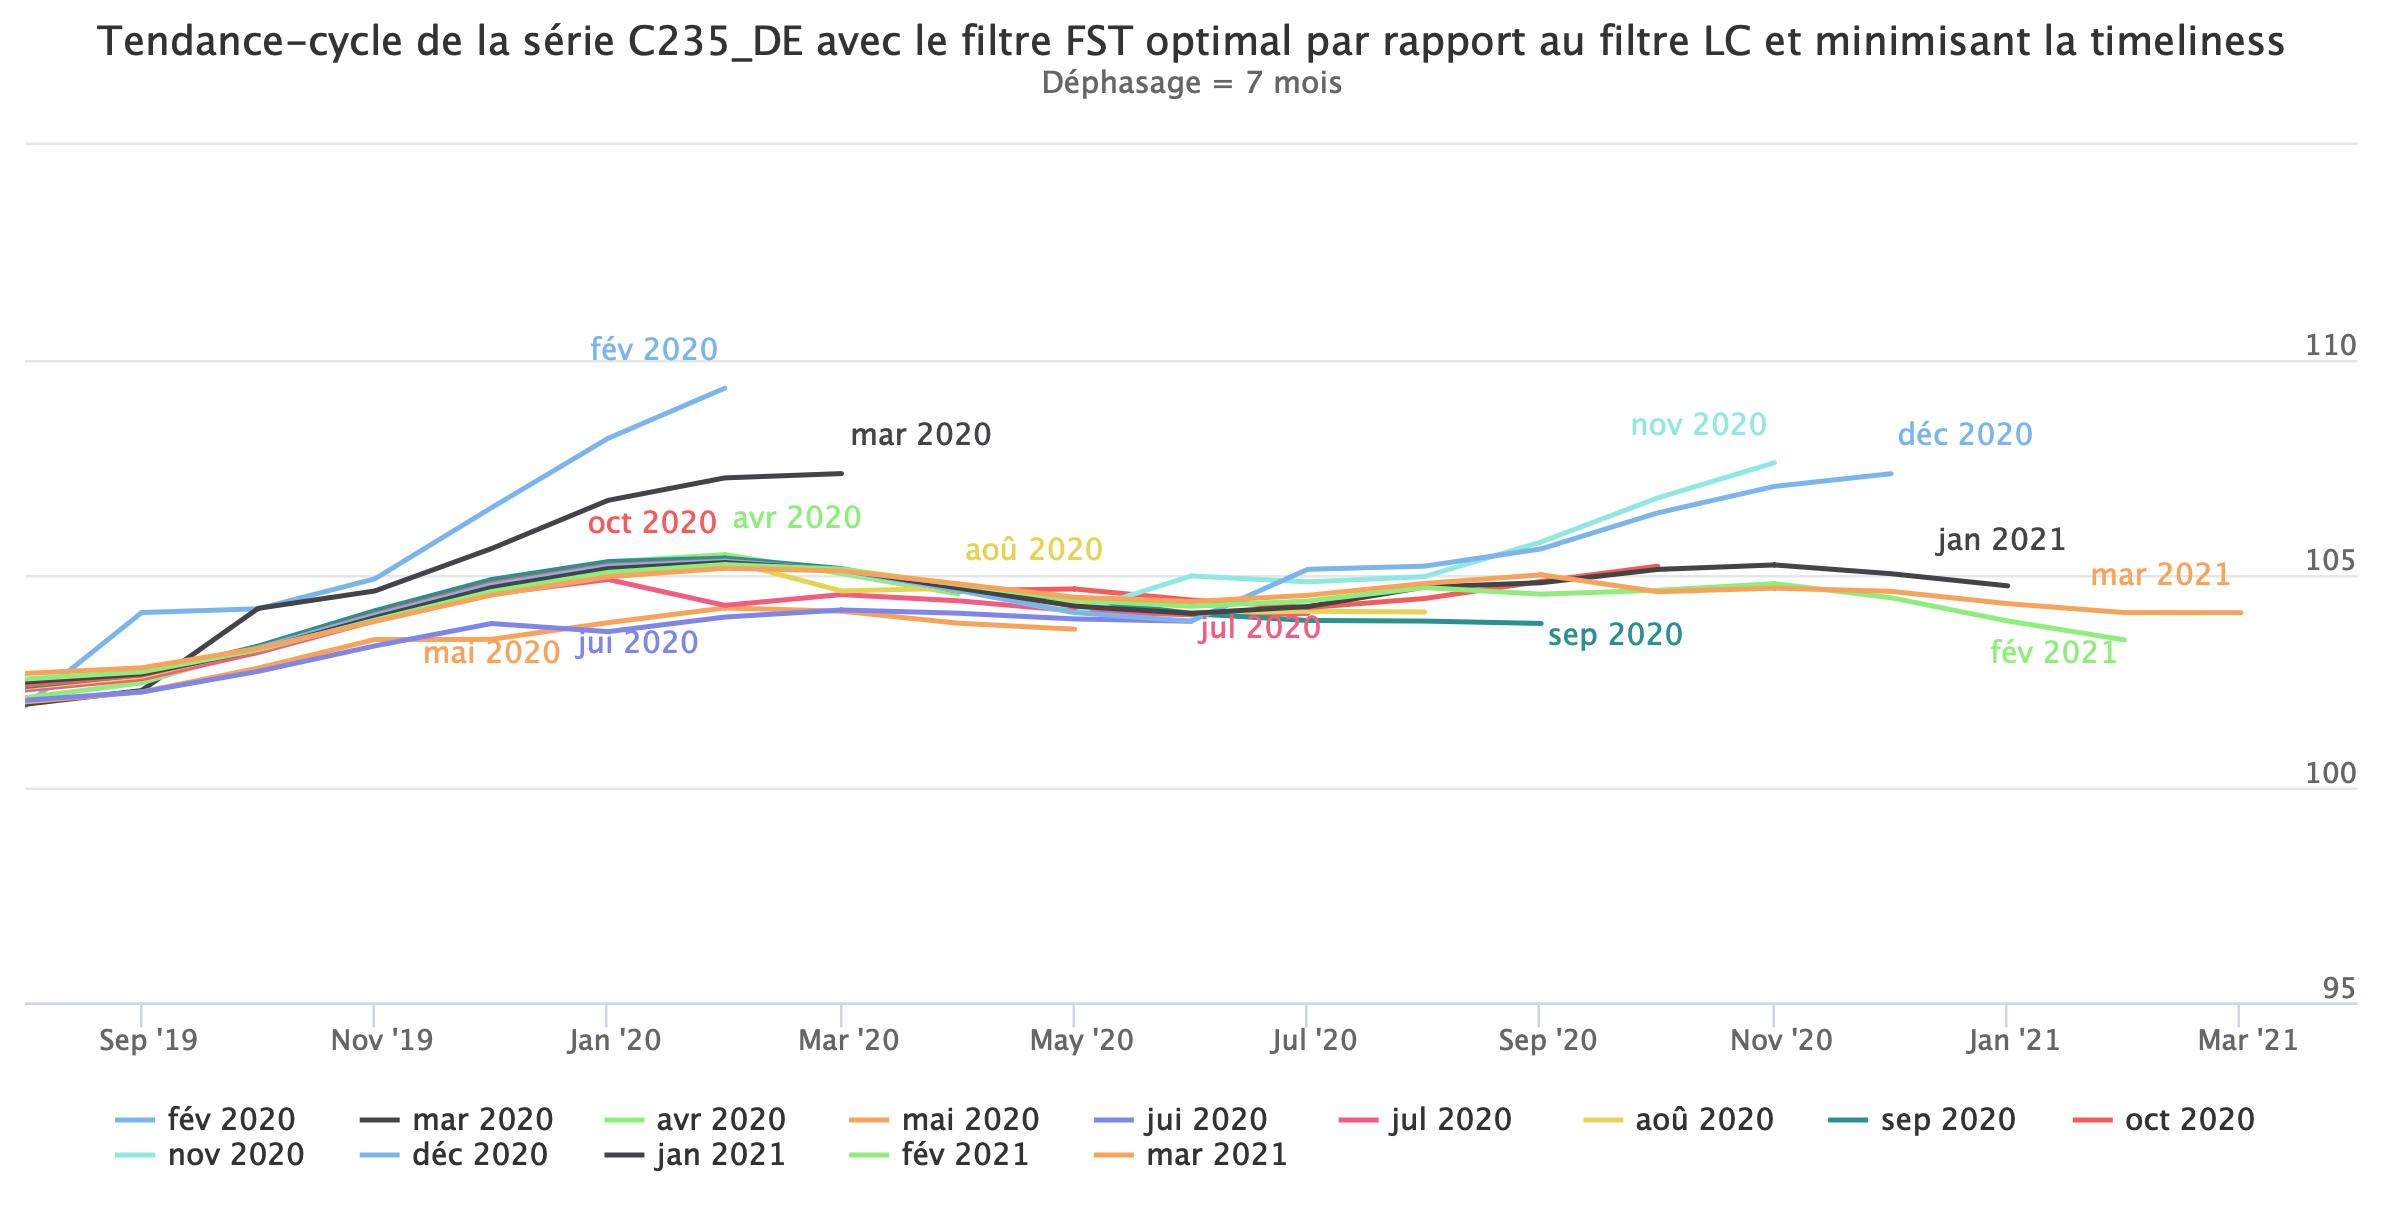
\includegraphics[width=0.9\linewidth,]{img/simulations/c235_de_fst_lc} 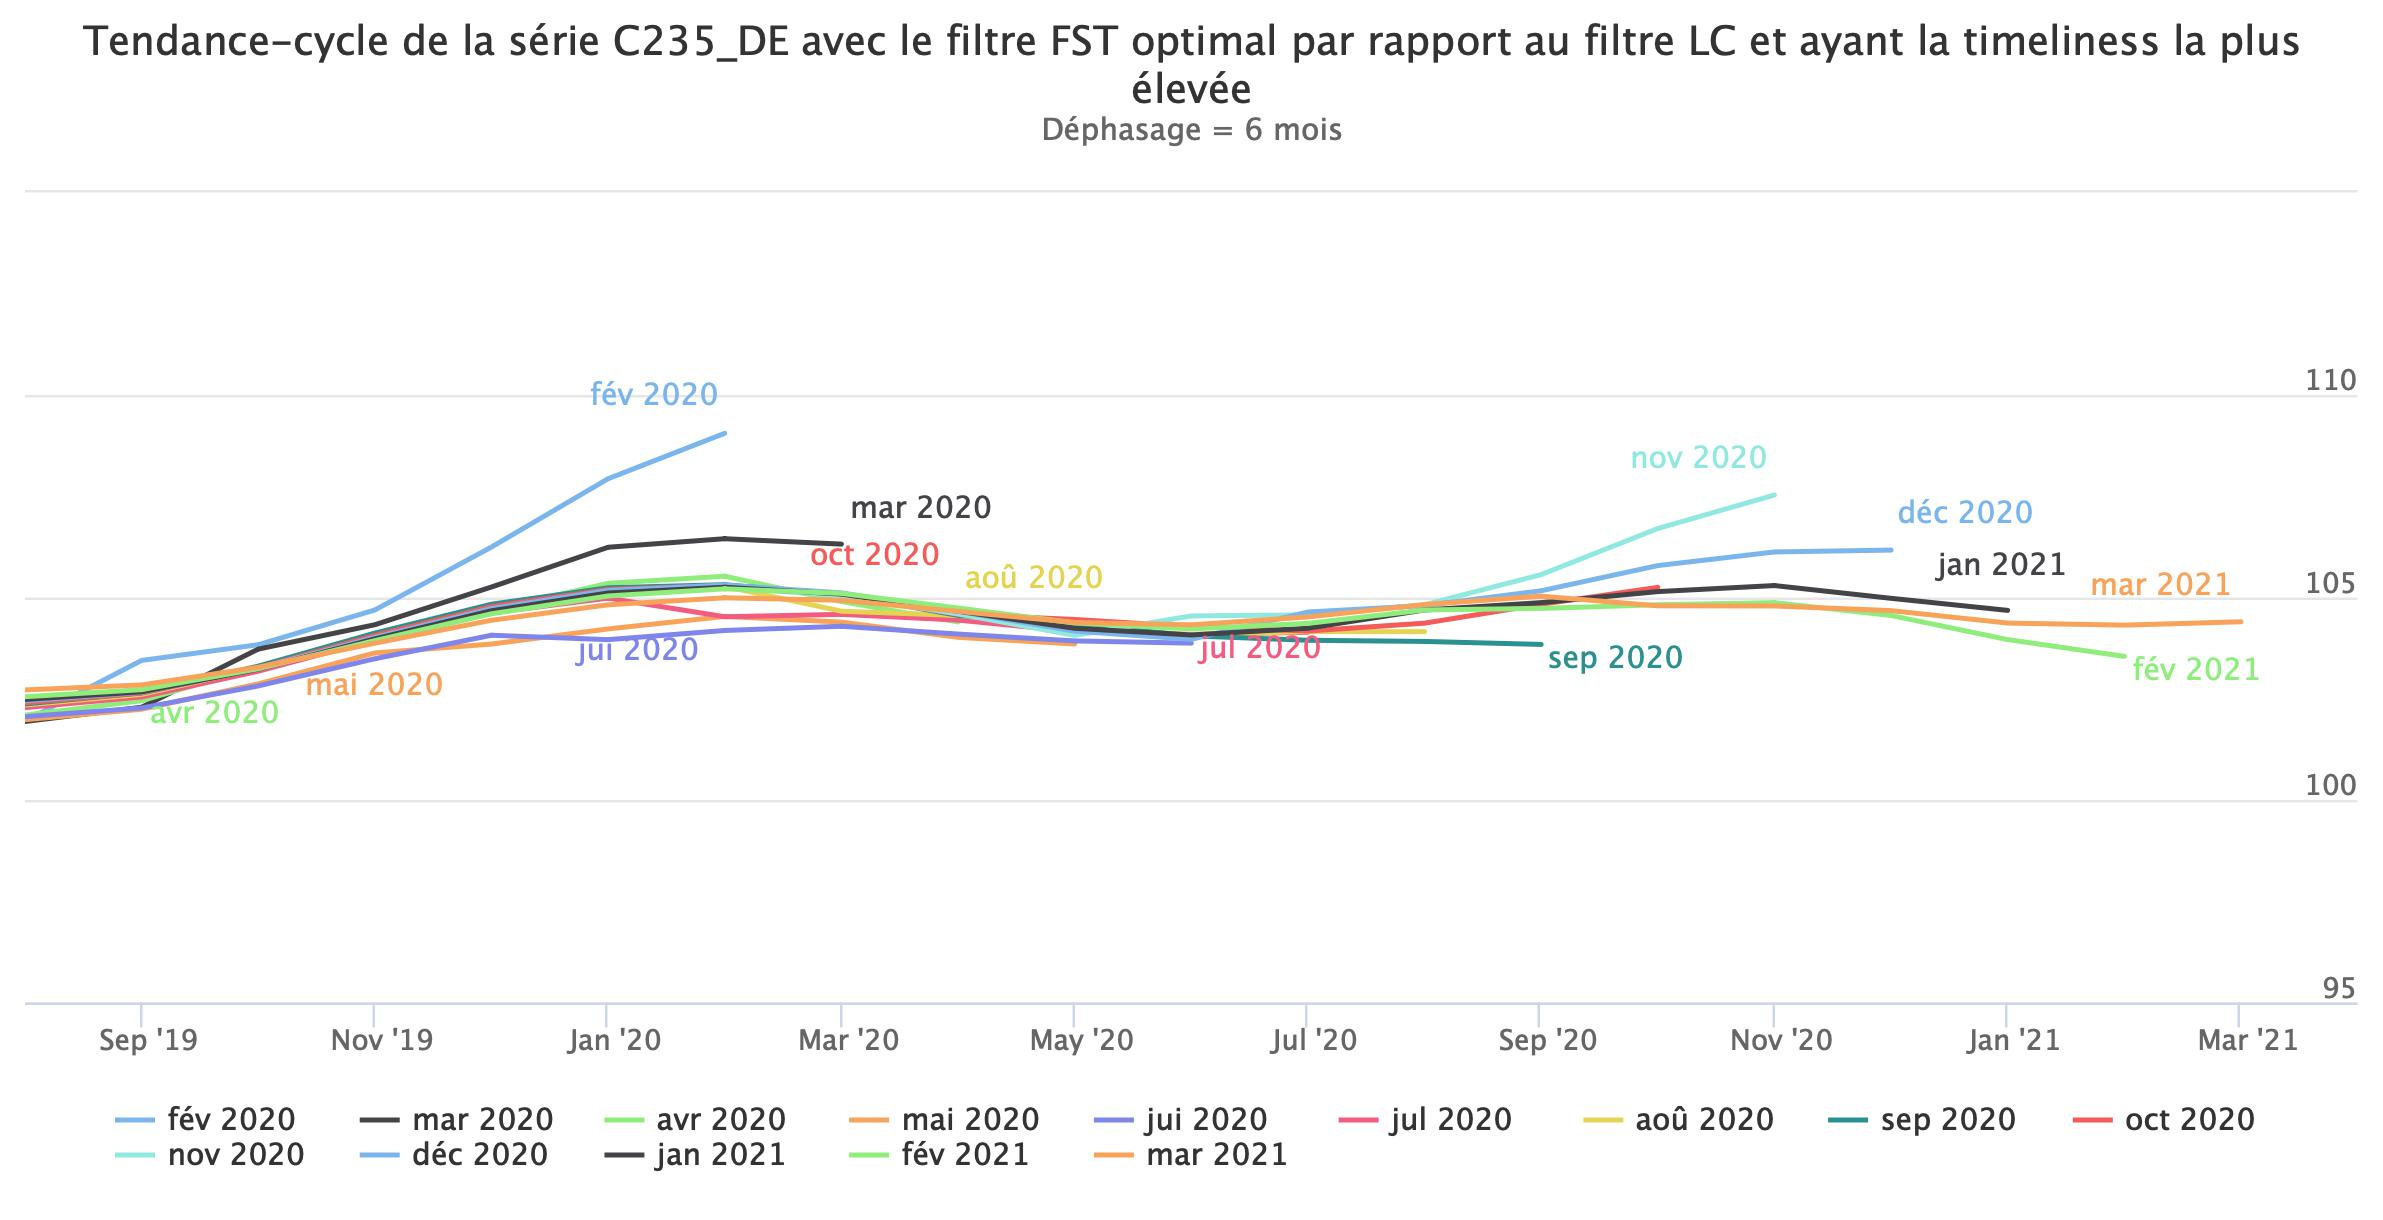
\includegraphics[width=0.9\linewidth,]{img/simulations/c235_de_fst_lc_min} 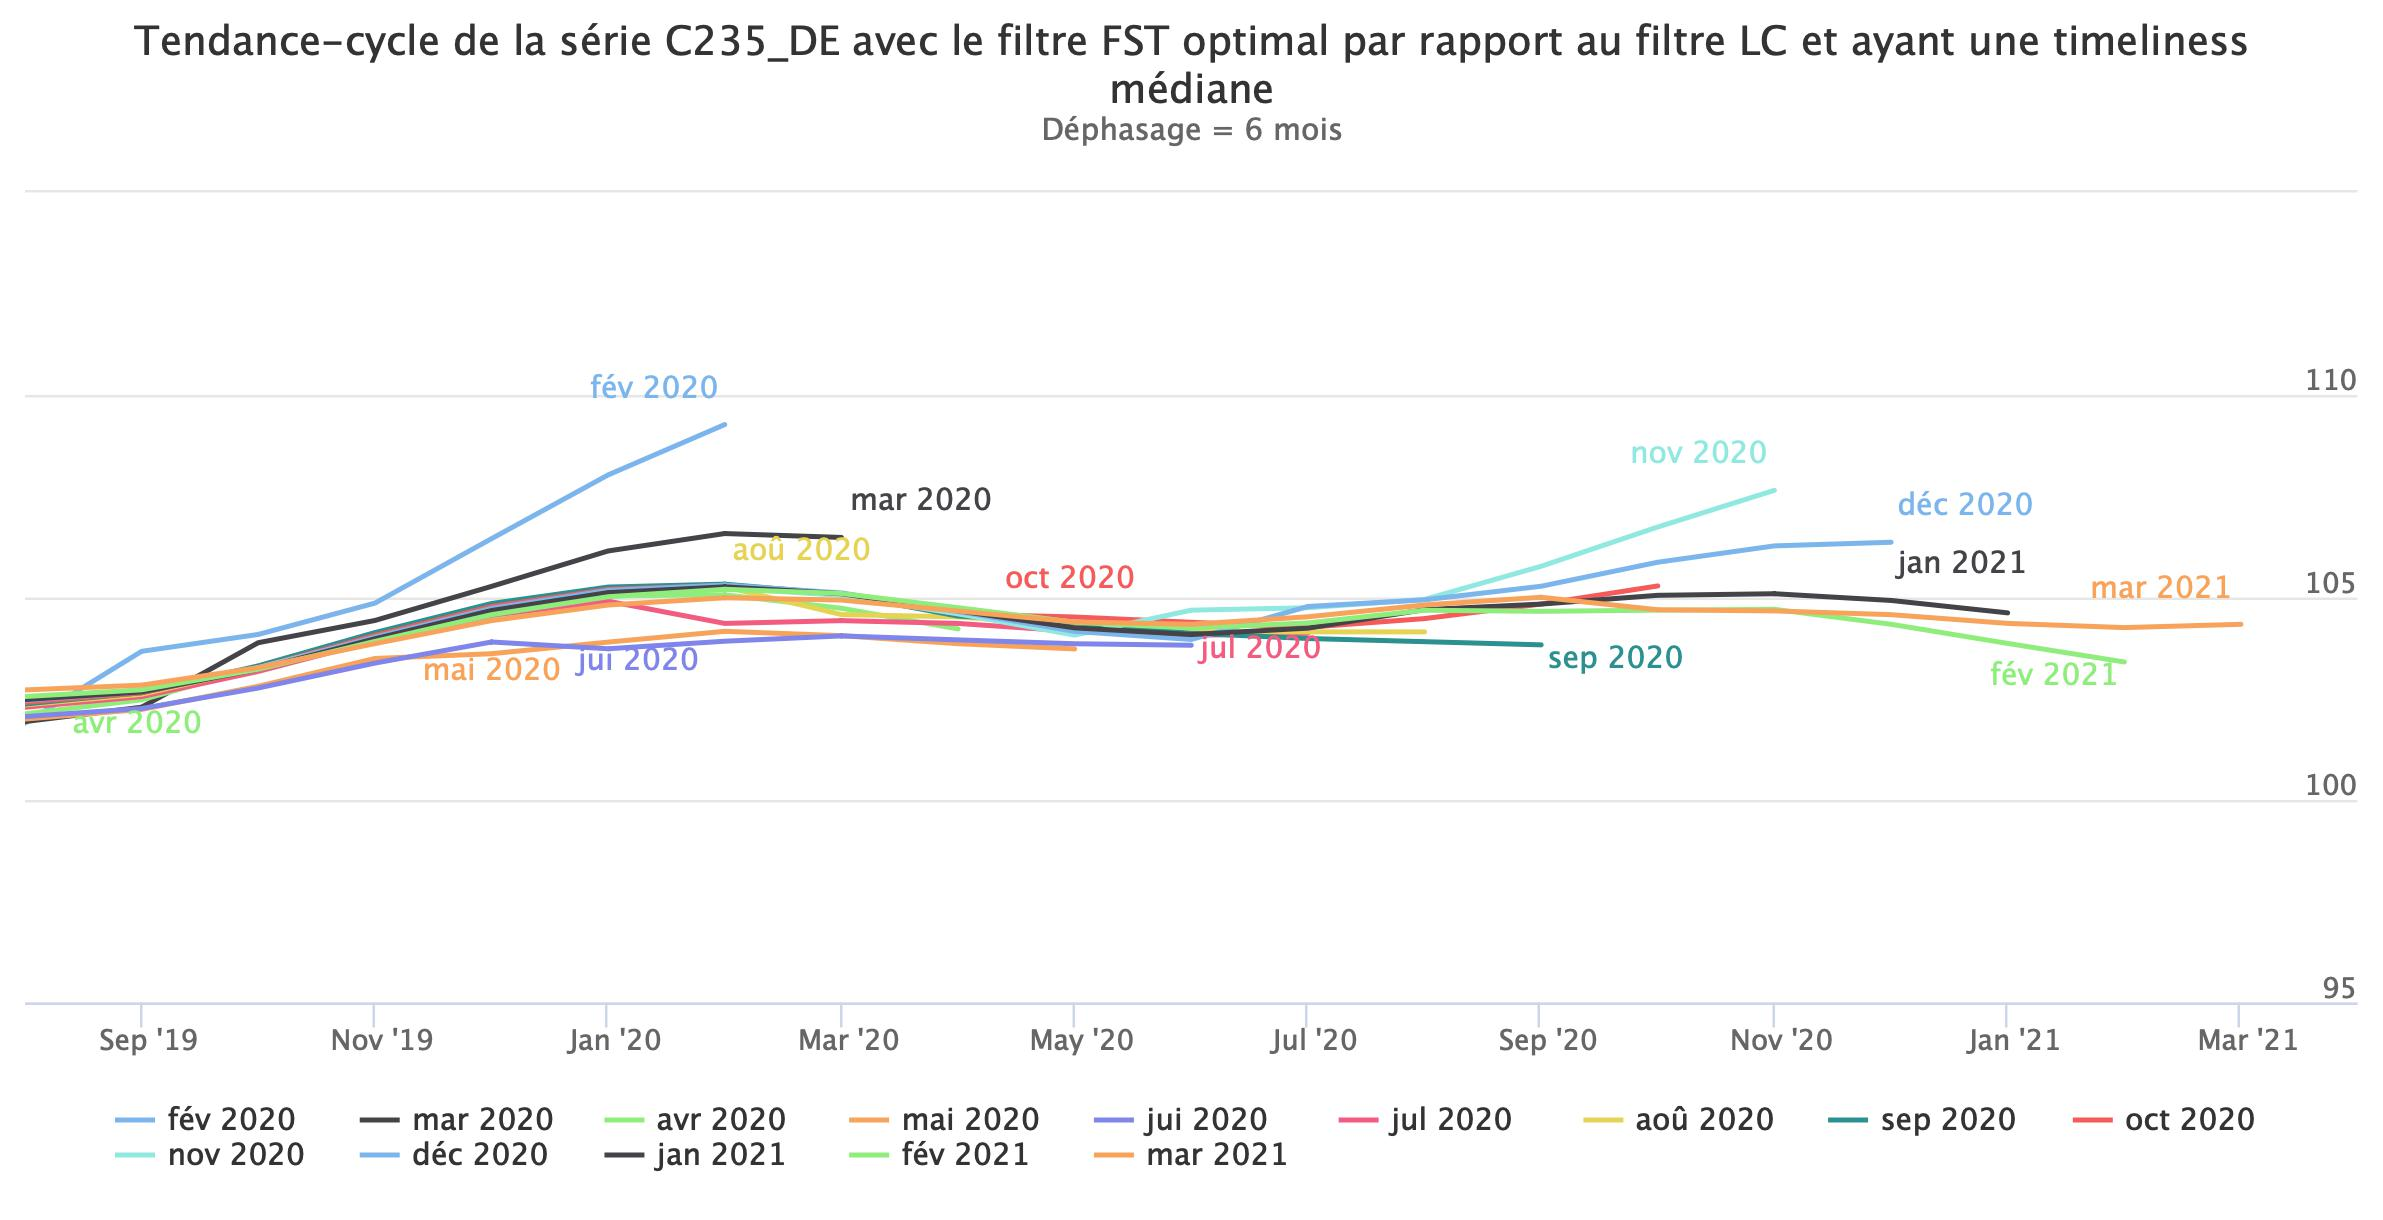
\includegraphics[width=0.9\linewidth,]{img/simulations/c235_de_fst_lc_med} 

}

\caption[Estimations de la tendance-cycle pour l'indice de production industriel dans la fabrication de ciment, chaux et plâtre (C235) en Allemagne (point de retournement en février 2020)]{Estimations de la tendance-cycle pour l'indice de production industriel dans la fabrication de ciment, chaux et plâtre (C235) en Allemagne (point de retournement en février 2020).}\label{fig:c235dep3}

\footnotesize
\normalsize\end{figure}

\begin{figure}[H]

{\centering 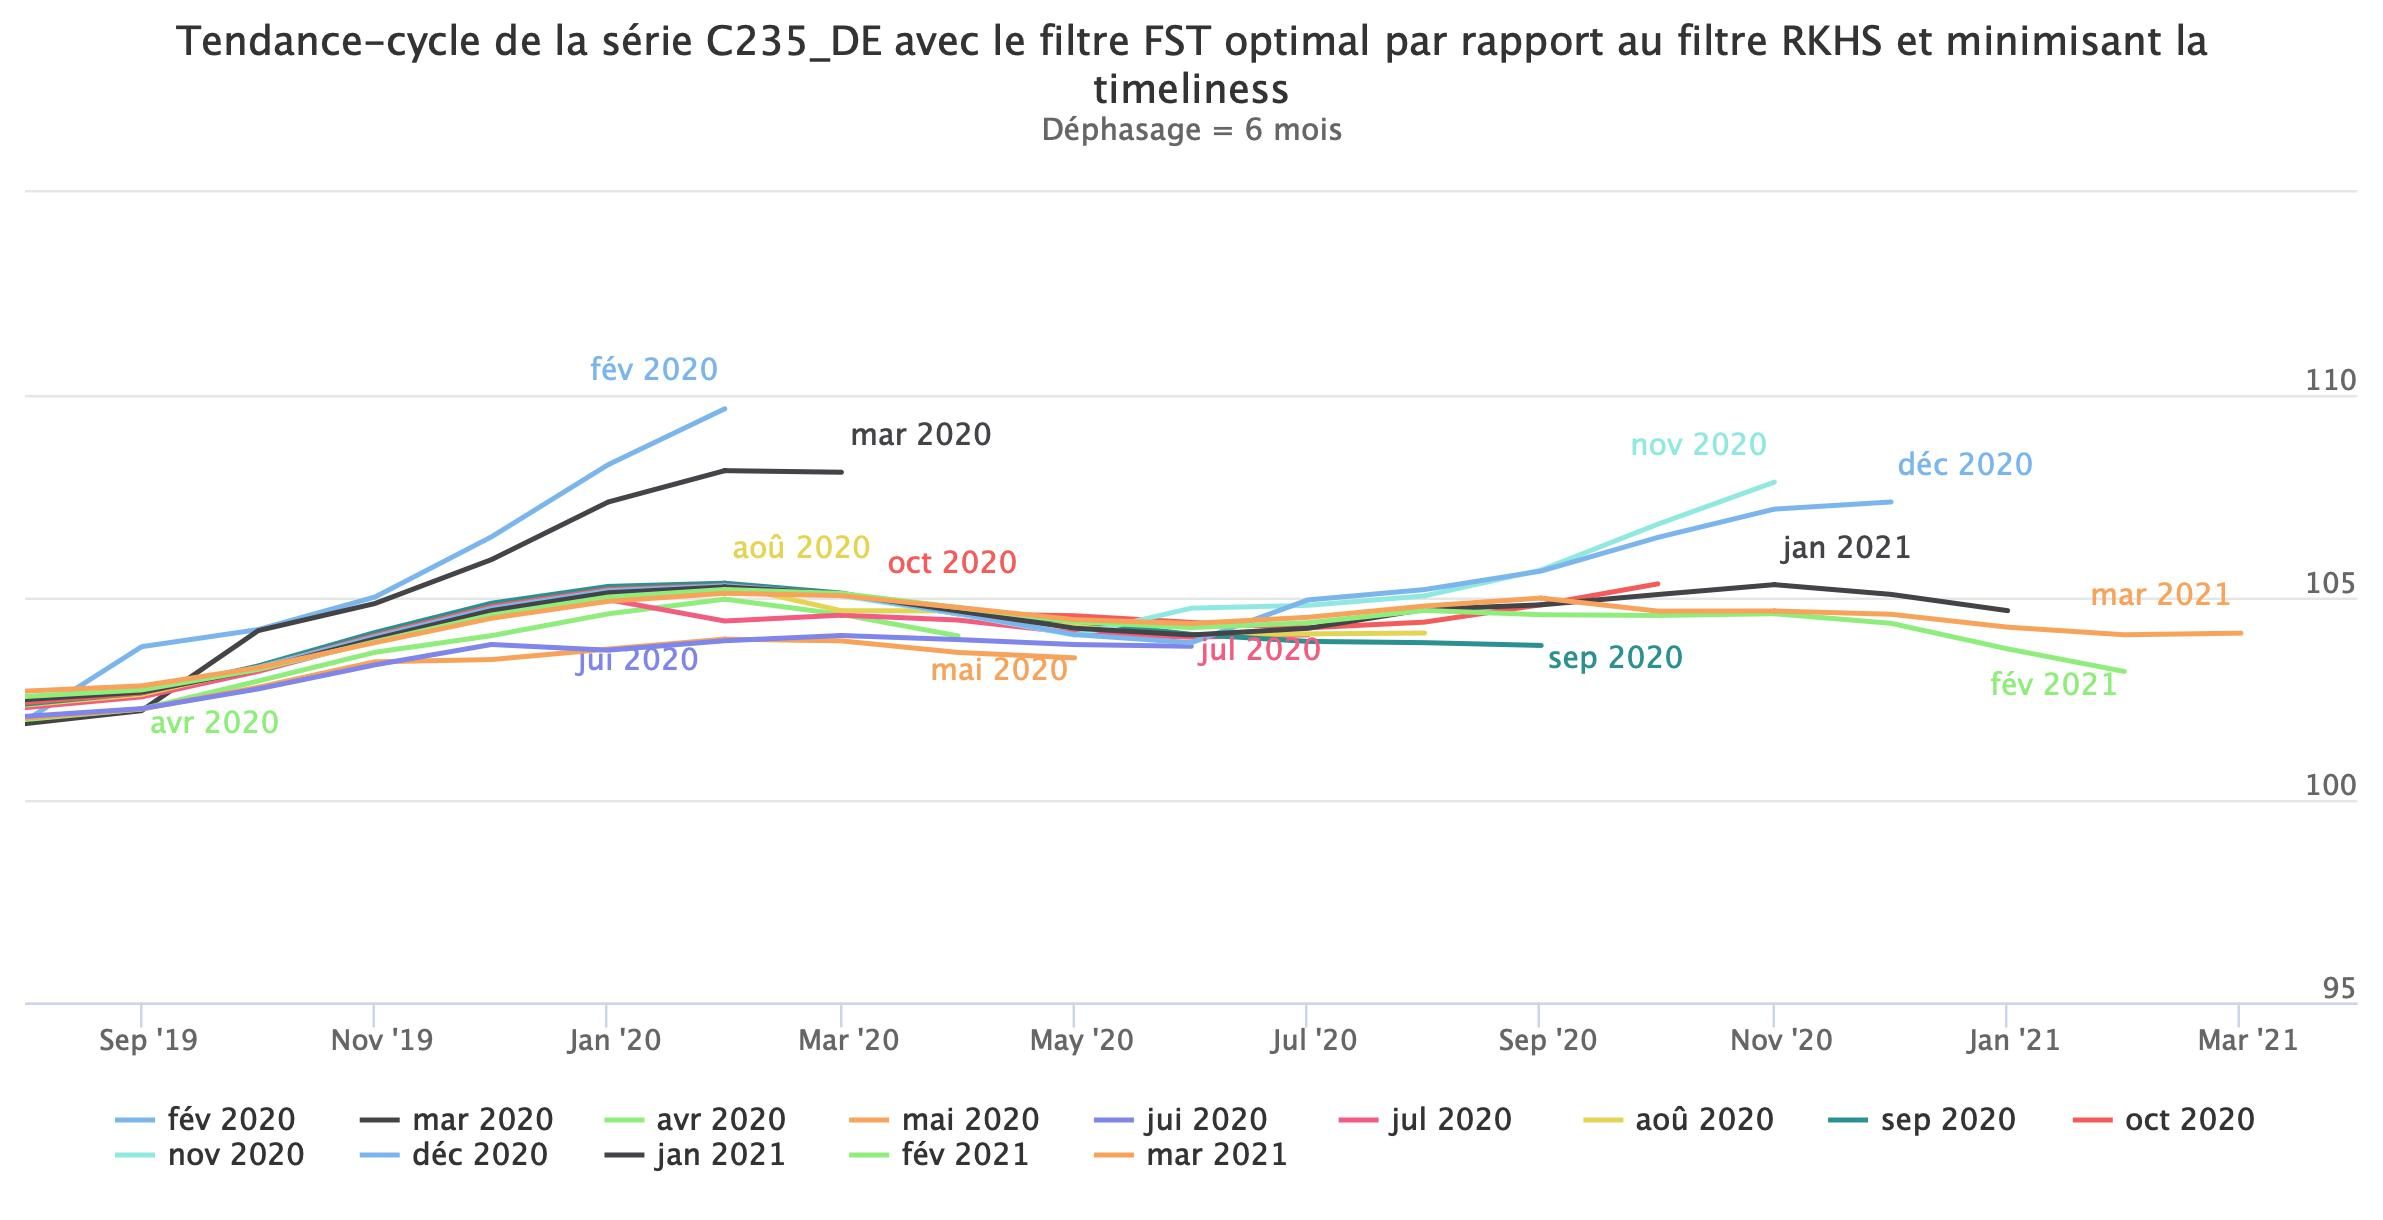
\includegraphics[width=0.9\linewidth,]{img/simulations/c235_de_fst_rkhs_timeliness} 

}

\caption[Estimations de la tendance-cycle pour l'indice de production industriel dans la fabrication de ciment, chaux et plâtre (C235) en Allemagne (point de retournement en février 2020)]{Estimations de la tendance-cycle pour l'indice de production industriel dans la fabrication de ciment, chaux et plâtre (C235) en Allemagne (point de retournement en février 2020).}\label{fig:c235dep4}

\footnotesize
\normalsize\end{figure}

\begin{figure}[H]

{\centering 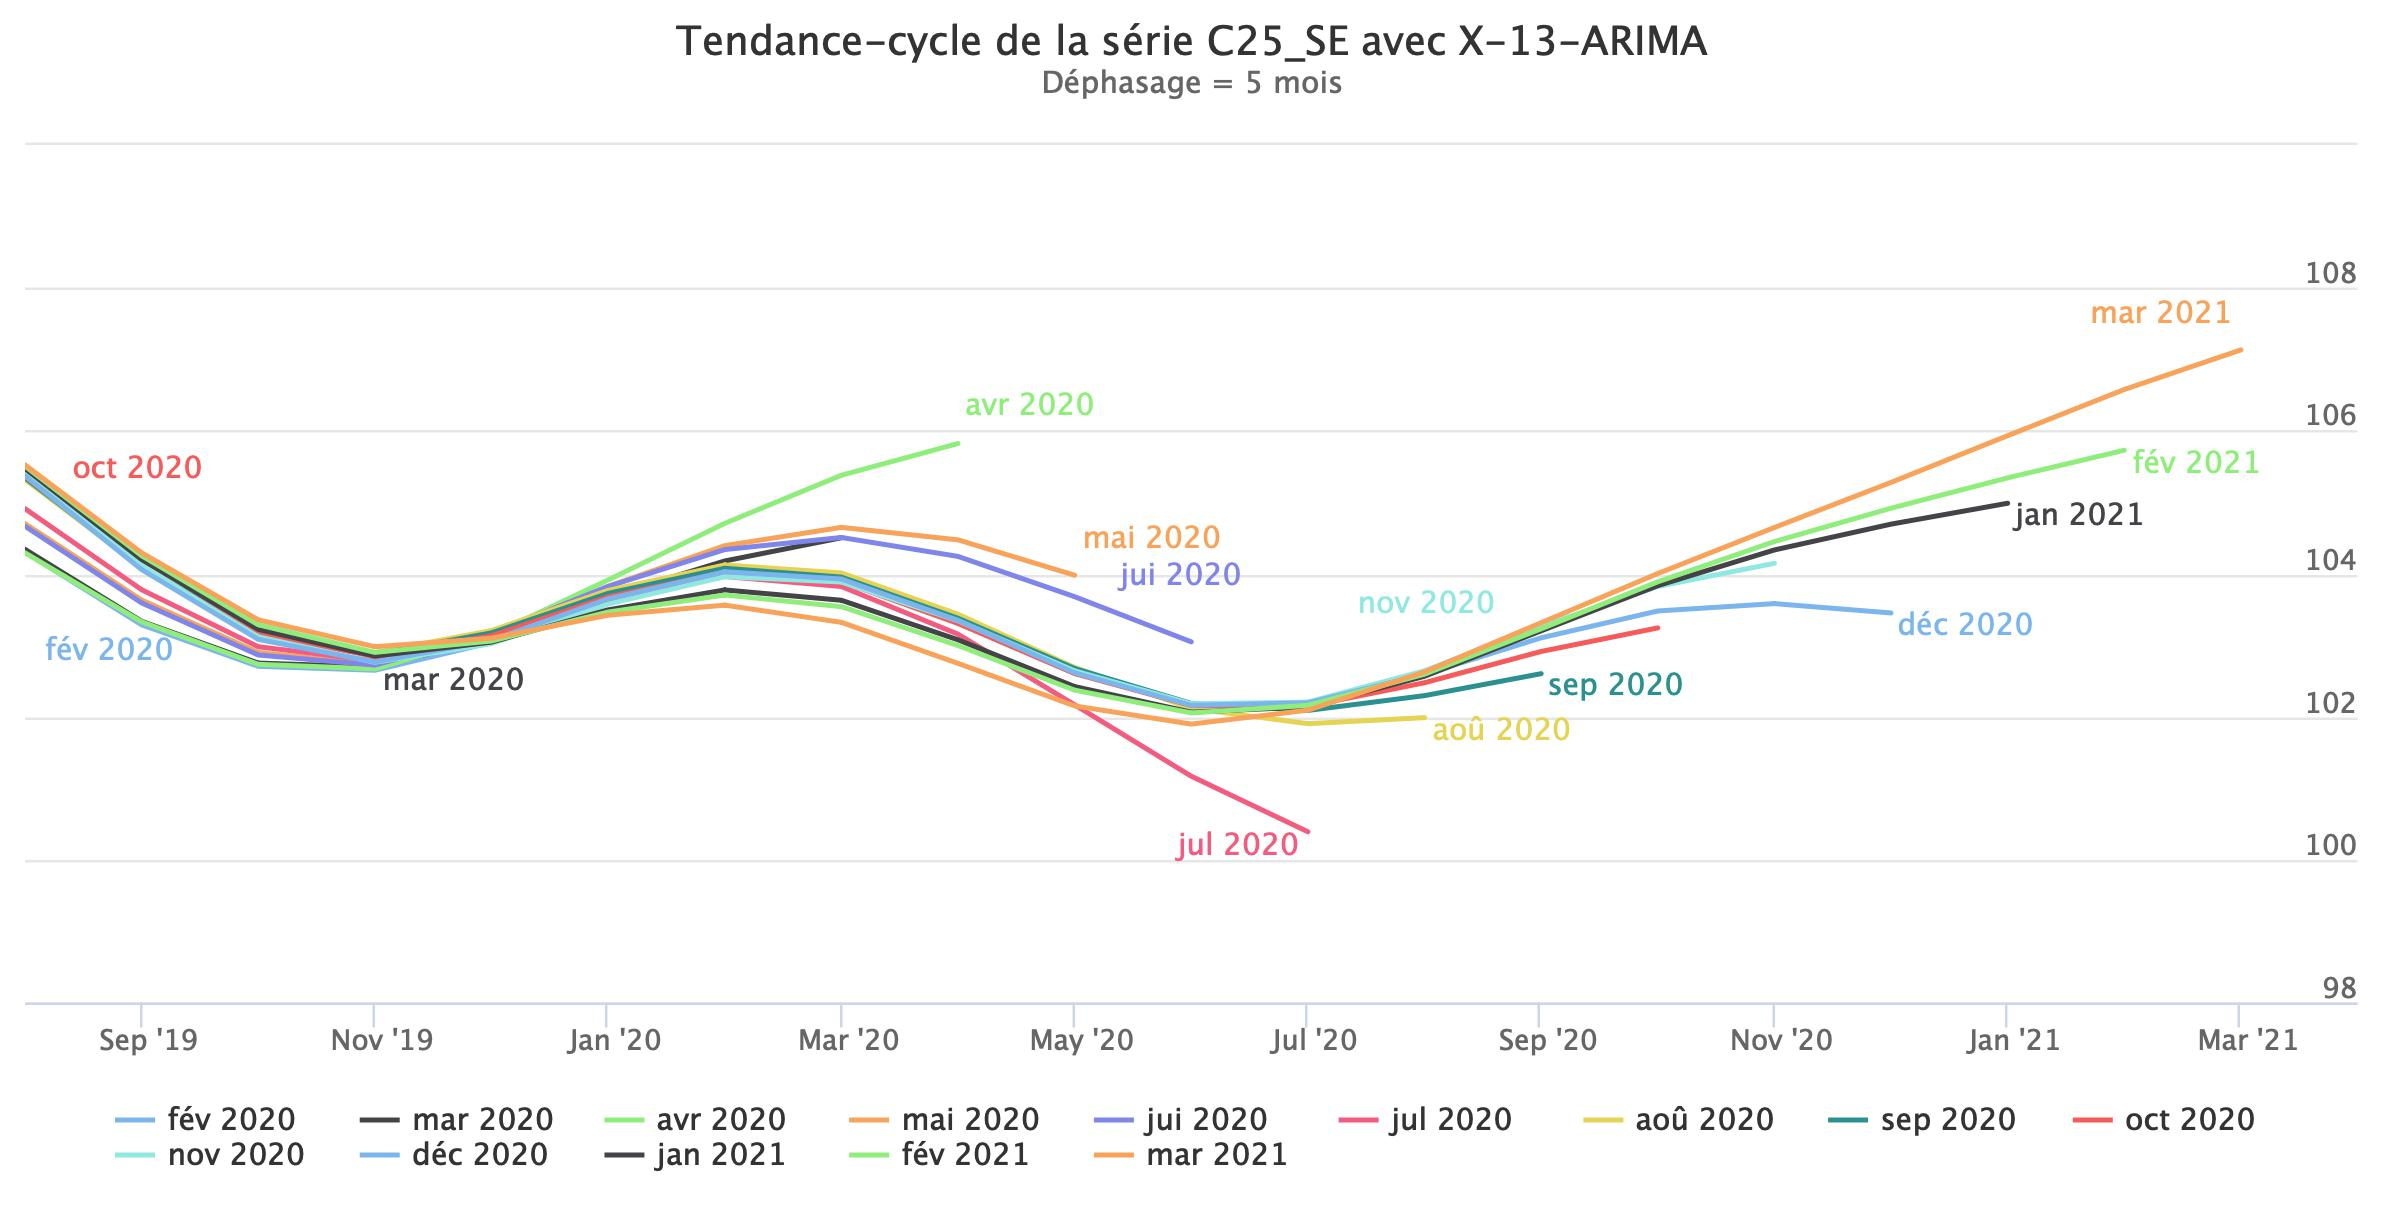
\includegraphics[width=0.9\linewidth,]{img/simulations/c25_se_x13} 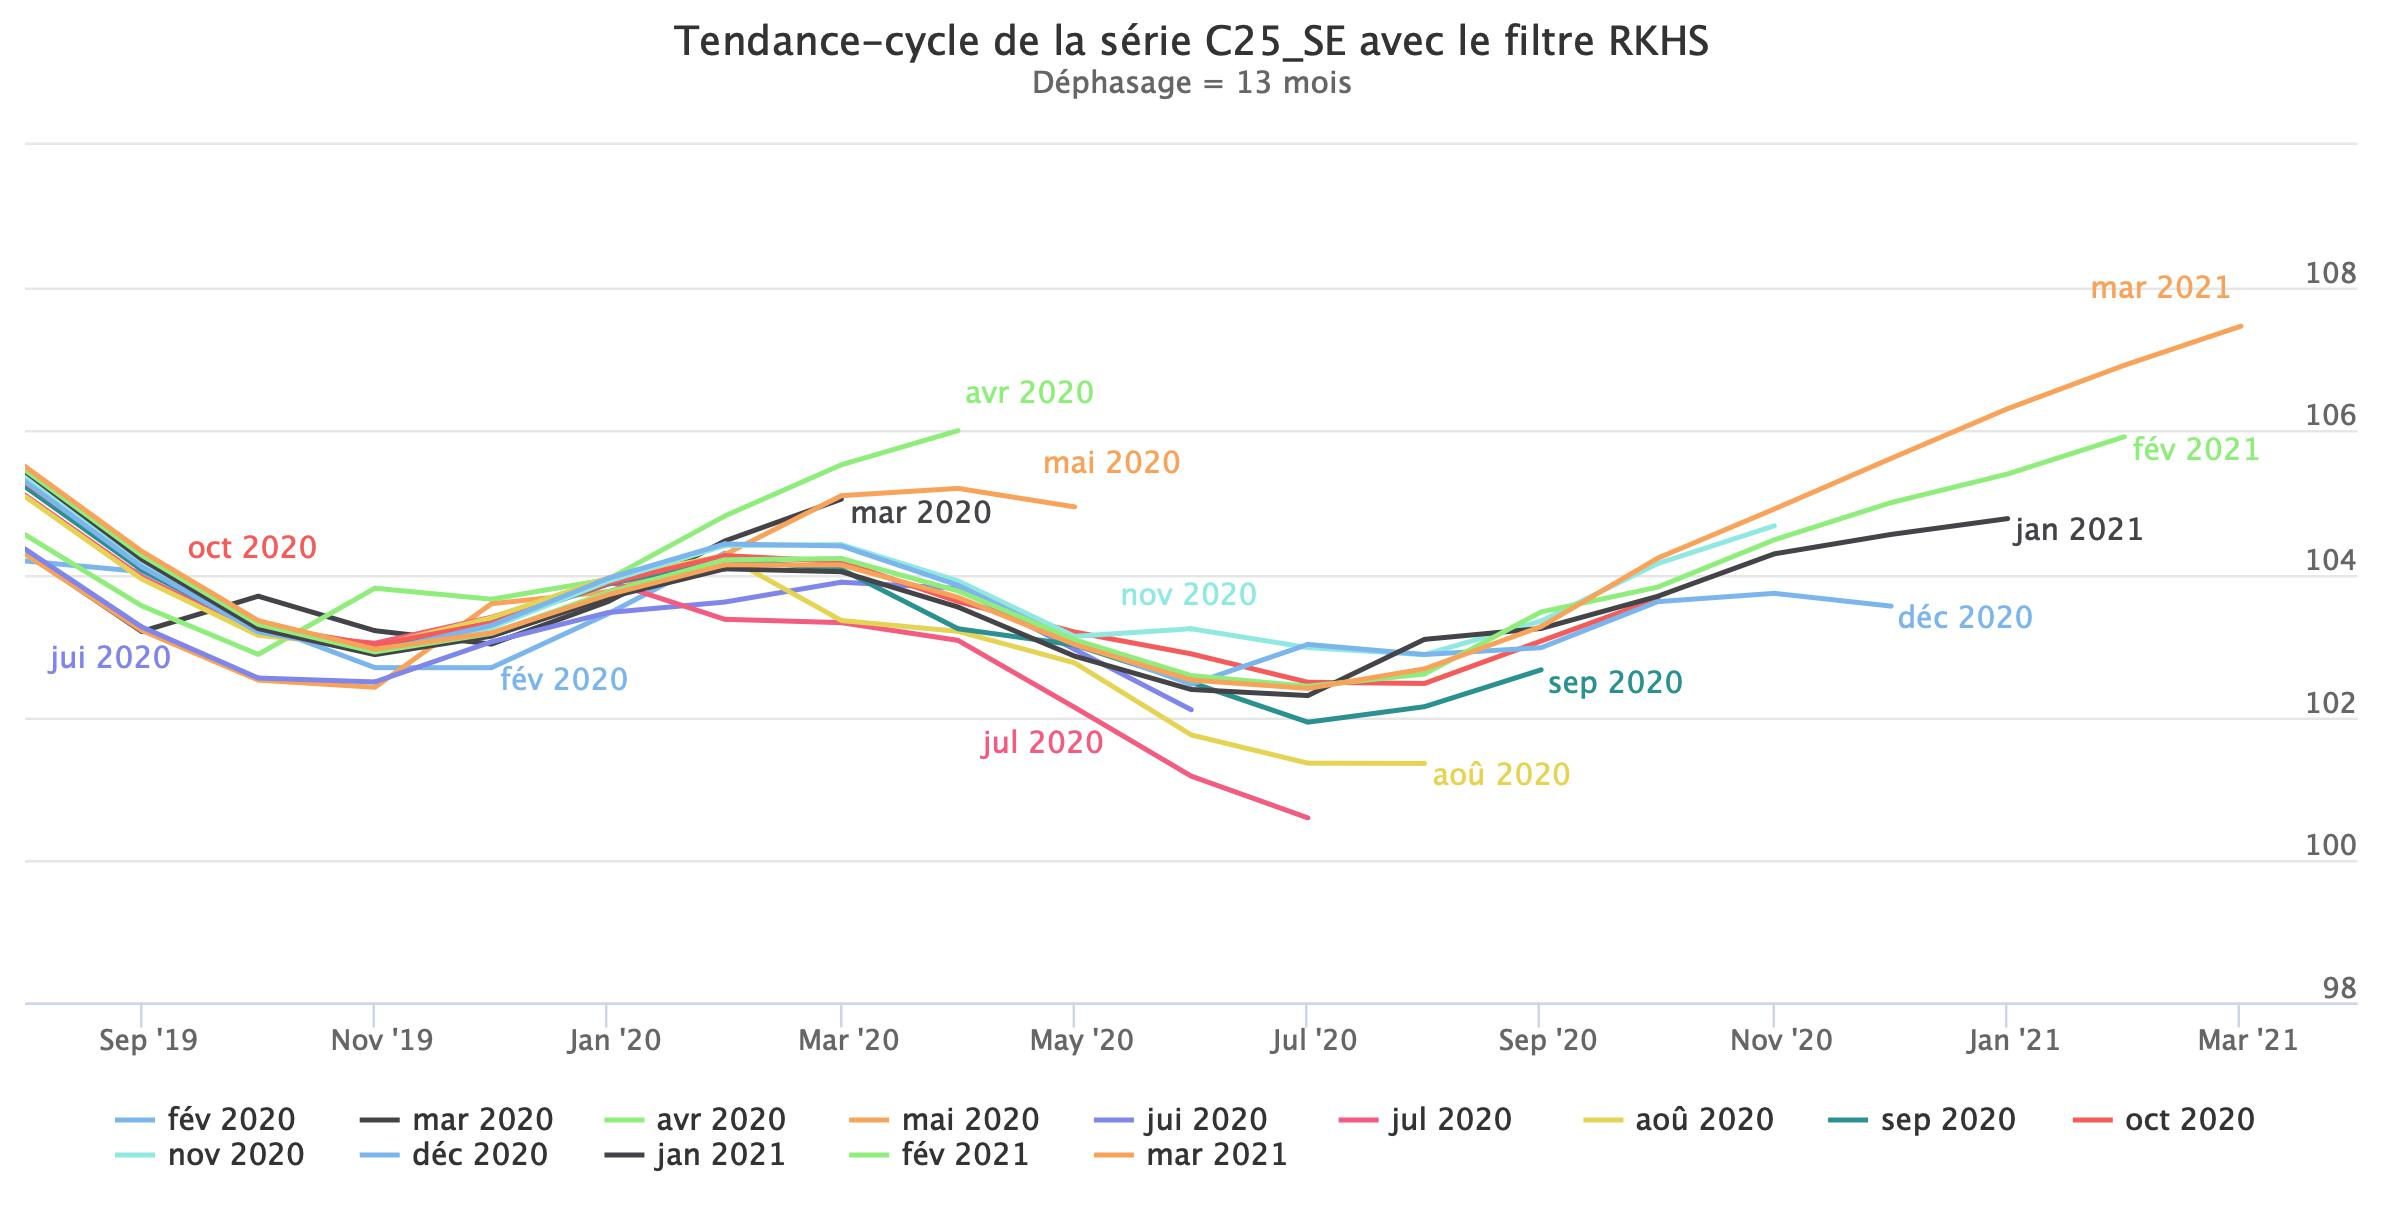
\includegraphics[width=0.9\linewidth,]{img/simulations/c25_se_rkhs_timeliness} 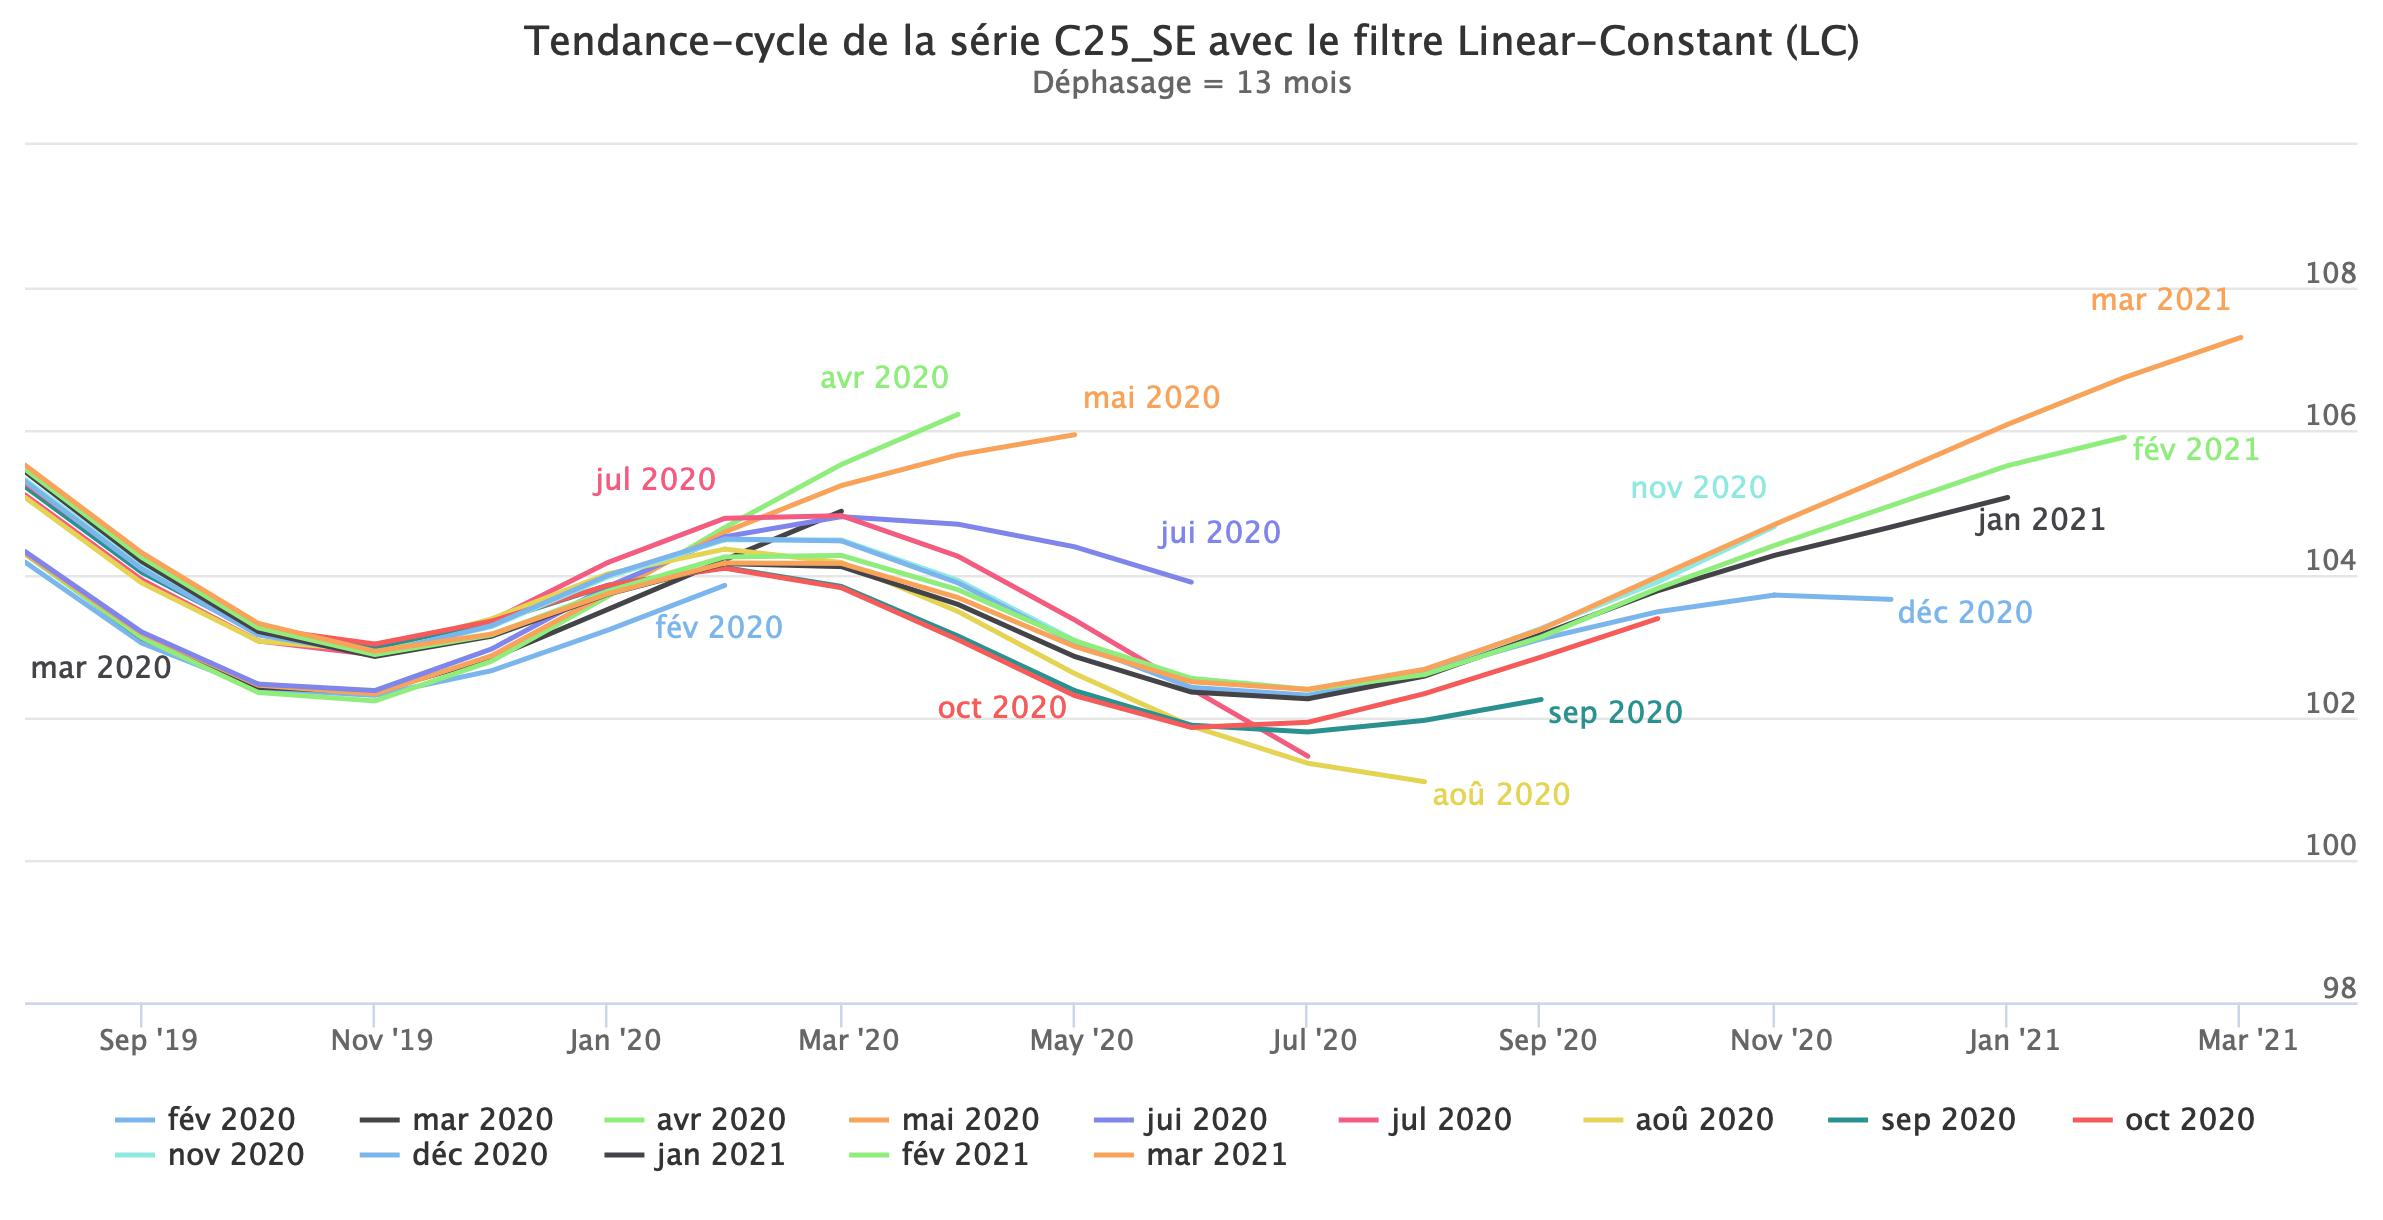
\includegraphics[width=0.9\linewidth,]{img/simulations/c25_se_lc} 

}

\caption[Estimations de la tendance-cycle pour l'indice de production industriel dans la fabrication de produits métalliques, à l'exception des machines et des équipements (C25) en Suède (point de retournement en février 2020)]{Estimations de la tendance-cycle pour l'indice de production industriel dans la fabrication de produits métalliques, à l'exception des machines et des équipements (C25) en Suède (point de retournement en février 2020).}\label{fig:c25sep1}

\footnotesize
\normalsize\end{figure}

\begin{figure}[H]

{\centering 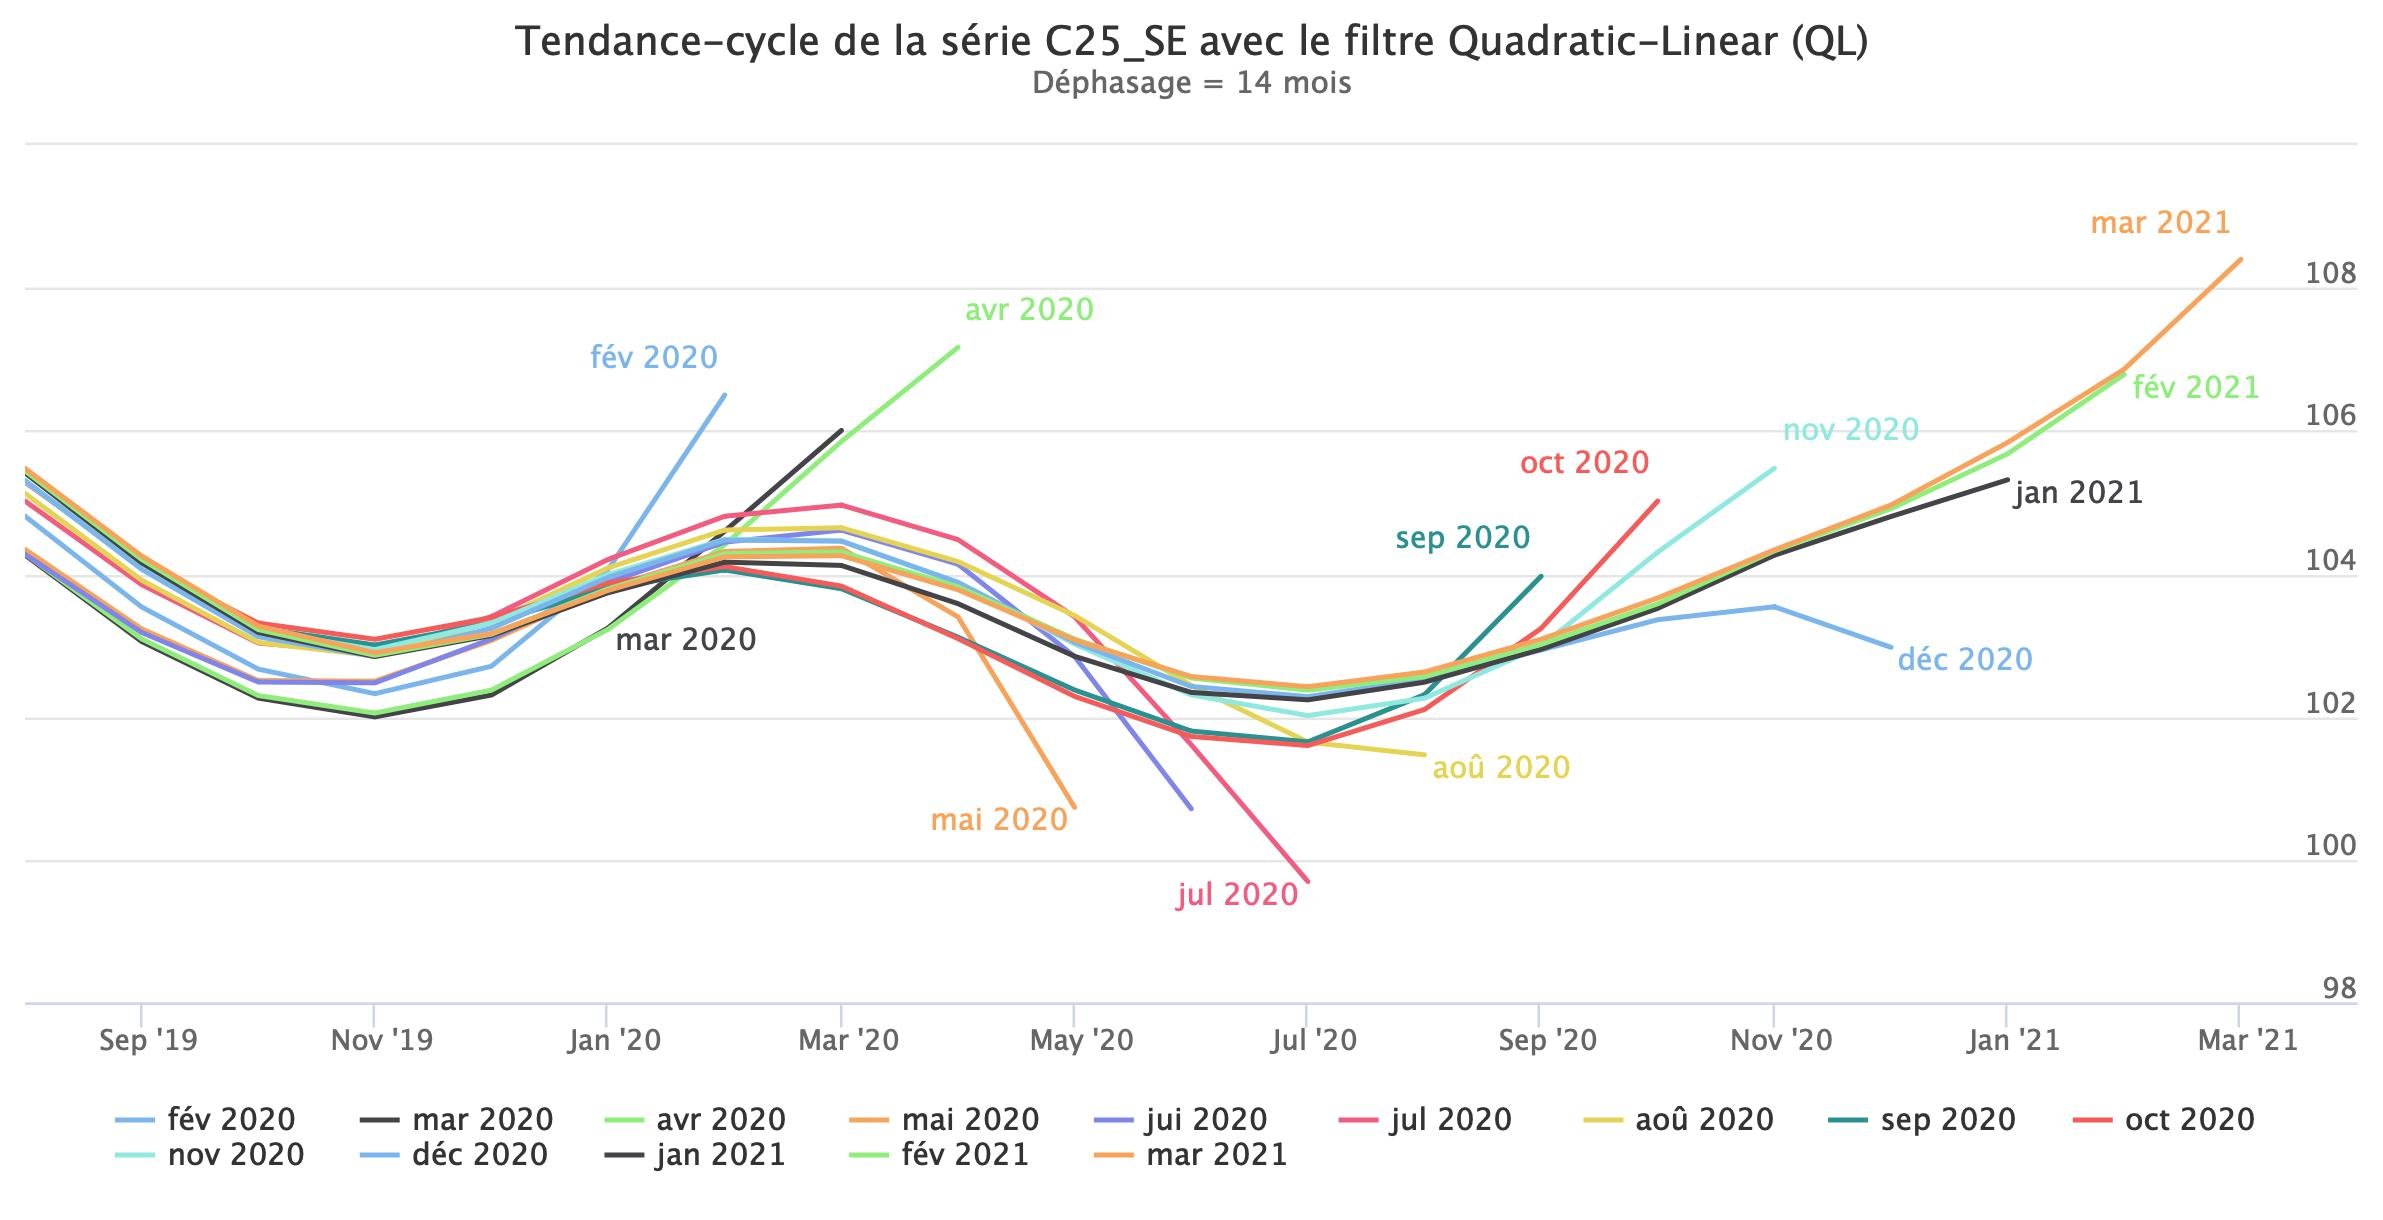
\includegraphics[width=0.9\linewidth,]{img/simulations/c25_se_ql} \includegraphics[width=0.9\linewidth,]{img/simulations/c25_se_cq} \includegraphics[width=0.9\linewidth,]{img/simulations/c25_se_daf} 

}

\caption[Estimations de la tendance-cycle pour l'indice de production industriel dans la fabrication de produits métalliques, à l'exception des machines et des équipements (C25) en Suède (point de retournement en février 2020)]{Estimations de la tendance-cycle pour l'indice de production industriel dans la fabrication de produits métalliques, à l'exception des machines et des équipements (C25) en Suède (point de retournement en février 2020).}\label{fig:c25sep2}

\footnotesize
\normalsize\end{figure}

\begin{figure}[H]

{\centering \includegraphics[width=0.9\linewidth,]{img/simulations/c25_se_fst_lc} \includegraphics[width=0.9\linewidth,]{img/simulations/c25_se_fst_lc_min} \includegraphics[width=0.9\linewidth,]{img/simulations/c25_se_fst_lc_med} 

}

\caption[Estimations de la tendance-cycle pour l'indice de production industriel dans la fabrication de produits métalliques, à l'exception des machines et des équipements (C25) en Suède (point de retournement en février 2020)]{Estimations de la tendance-cycle pour l'indice de production industriel dans la fabrication de produits métalliques, à l'exception des machines et des équipements (C25) en Suède (point de retournement en février 2020).}\label{fig:c25sep3}

\footnotesize
\normalsize\end{figure}

\begin{figure}[H]

{\centering \includegraphics[width=0.9\linewidth,]{img/simulations/c25_se_fst_rkhs_timeliness} 

}

\caption[Estimations de la tendance-cycle pour l'indice de production industriel dans la fabrication de produits métalliques, à l'exception des machines et des équipements (C25) en Suède (point de retournement en février 2020)]{Estimations de la tendance-cycle pour l'indice de production industriel dans la fabrication de produits métalliques, à l'exception des machines et des équipements (C25) en Suède (point de retournement en février 2020).}\label{fig:c25sep4}

\footnotesize
\normalsize\end{figure}

\newpage

\printbibliography[heading=bibintoc]

\end{document}
